\documentclass[12pt,a4paper,oneside]{book}
\usepackage[a4paper,margin=1in]{geometry}
\usepackage[english]{babel}
\usepackage[utf8]{inputenc}
\usepackage[nottoc]{tocbibind}
\usepackage{amssymb}
\usepackage{hyperref}
\usepackage[nameinlink]{cleveref}
\usepackage{graphicx}
\usepackage{fancyhdr}
\usepackage{multirow}
\usepackage[font=small]{caption}
\usepackage{xcolor}
\usepackage{lscape}
\usepackage{subcaption}
\usepackage{floatrow}
\usepackage{sectsty}
\usepackage[skip=10pt, indent=0pt]{parskip}
\usepackage[explicit]{titlesec}
\usepackage[numbers, sort&compress ]{natbib}
\usepackage{minted}
\usepackage{algorithm}
\usepackage{algpseudocode}
\usepackage{tikz, blindtext}

\definecolor{scarlat}{HTML}{c72125}
\allsectionsfont{\sffamily}
\chapterfont{\sffamily\color{scarlat}}

\pagestyle{fancy}
\fancyhf{}
\fancyfoot[L]{\thepage}
\fancyfoot[R]{\leftmark}
\fancyfoot[C]{}
\renewcommand{\headrulewidth}{0pt}
\renewcommand{\footrulewidth}{0.5pt}
\renewcommand{\chaptermark}[1]{\markboth{#1}{}}

\fancypagestyle{plain}{%
    \fancyhf{}
    \fancyfoot[C]{\thepage}
    \fancyfoot[L,R]{}
    \renewcommand{\headrulewidth}{0pt}
    \renewcommand{\footrulewidth}{0.5pt}
}

\newskip\bigskipamount \bigskipamount =20pt plus 4pt minus 4pt
% \setcounter{tocdepth}{1}
\setcounter{secnumdepth}{3}

\begin{document}
\pagenumbering{roman}

\begin{titlepage}
\centering

\includegraphics[width=0.7\linewidth]{graphics/tue-logo.png}\par
Department of Mathematics and Computer Science

\vspace{3cm}

{\sffamily\LARGE\textbf{
A Study on the Impact of Different Algorithms in Blockchain-based Federated Learning Systems Using a Modular Framework
}}

\par\vspace{2cm}
{\large\textit{Master Thesis}}\\
\vspace{0.2cm}
{\large Henrique Afonso Coelho Dias}

\vspace{2cm}

\textbf{Supervisor} \\
\vspace{0.1cm}
prof. dr. ir. N. Meratnia

\par

\textbf{Assessment Committee} \\
\vspace{0.1cm}
prof. dr. ir. N. Meratnia \\
prof. dr. ir. P.H.F.M. Verhoeven \\
prof. dr. ir. S. Sciancalepore \\

\vfill

{Eindhoven, September 2022}

\end{titlepage}

\chapter*{Abstract}\label{chapter:abstract}
Blockchain-based Federated Learning eliminates the central coordinator of classical Federated Learning networks, allowing multiple distributed clients to cooperate on the same Machine Learning model, without a single point of failure in the network. It is common to score each client's submission in order to determine if it is a good contribution to the global model. With Federated Learning being increasingly adopted in IoT networks, where low powered devices with low resources are the norm, it is important to ensure that certain aspects of the system that can be changed consume the least amount of resources. The current literature has very little information regarding how different aspects impact the system. Additionally, there is no publicly available framework that can be used to implement a Blockchain-based Federated Learning system.

In this thesis, we design and implement the first modular open-source framework for Blockchain-based Federated Learning using Ethereum and TensorFlow. This framework can be easily adapted to support multiple architectures, as well as different scoring, aggregation and privacy techniques. With this framework, we proceed to do the first known analysis of how different aspects of Blockchain-based Federated Learning, such as consensus algorithms, participation selection techniques and scoring techniques, impact the accuracy, execution time and communication and computation costs. Additionally, the same analysis is done per each scoring technique regarding the impact of the number of clients and privacy techniques. Finally, we also provide a proof of concept of how the framework can be adapted to support, not only Horizontal Federated Learning, but also Vertical Federated Learning.

\tableofcontents

\listoffigures

\listoftables

\chapter{Introduction}\label{chapter:introduction}
\pagenumbering{arabic}
Machine Learning (ML) has revolutionized the way we think and work with data, opening way to new techniques and explorations. ML models can be powerful tools to predict things that would otherwise require high amounts of effort, either human or computational. As an example, we can think about image recognition in healthcare that can help medical professionals diagnose disorders. Another example could be smart watch sensor data that can help train models to detect abnormal heart rates or walking patterns. Even though models such as these can be very helpful, they have to be trained with high amounts of good quality data in order for the model to perform accurately \cite{10.1145/3394486.3406477}. To address this issues, there are techniques that allow multiple parties to collaboratively train the same models.

In 2016, Google researchers attempted to build communication-efficient deep neural networks in decentralized data settings. The result of this work was the introduction of a new way of collaboratively training Machine Learning models, which they termed Federated Learning \cite{10.48550/arxiv.1602.05629}. Federated Learning (FL) allows multiple clients, in different locations, to cooperate on the same Machine Learning model without sharing their own data with each other. Instead of sharing the raw data, clients only share model parameters, such as weights. Both of this aspects bring some benefits. The first benefit is that, by not sharing raw data, models can preserve data privacy, allowing them to be trained on sensitive data. In addition, since model parameters are usually much smaller than the raw data, this also leads to less data being transported over the networks. Finally, since the data is distributed among different devices, a single powerful device is not required to train the model, as usually training models with smaller amounts of data is less computationally expensive.

Currently, most FL networks include a central server that coordinates the entire process and aggregates the model eights from each of the clients into a single model. This central coordinator is a single point of failure in the network, since it is always required to be online and behave correctly \cite{li_blockchain_2021, 10.48550/arxiv.2110.02182}. To address this, Blockchain-based Federated Learning techniques have been proposed. The following are some aspects and properties that Blockchain can bring to Federated Learning when combined:

\begin{itemize}
    \item \textit{Traceability and Auditability}. Due to the structure of the blockchain, it is possible to trace transactions to their original source, which can be useful for auditability purposes \cite{10.48550/arxiv.1902.01046, 10.48550/arxiv.2110.02182}.
    
    \item \textit{Data Immutability and Persistency}. Once transactions are added to the distributed ledger, it is nearly impossible to revert them or change their information \cite{10.48550/arxiv.1902.01046, qu_blockchain-enabled_2022}. This ensures that data is not changed and it can be retrieved after the fact.
    
    \item \textit{Decentralization}. The involvement of a central orchestrator is eliminated and the processing of the aggregation is replaced by multiple servers \cite{10.48550/arxiv.2009.09338, 9403374, 10.48550/arxiv.2110.02182, qu_blockchain-enabled_2022}. This improves the resilience and availability of the system.
    
    \item \textit{Authentication}. Blockchain ensures the authentication of data and messages due to the verification mechanisms in place, such as the usage of private keys to sign transactions \cite{qu_blockchain-enabled_2022}.
\end{itemize}

\section{Motivation}\label{intro:motivation}

In Blockchain-based Federated Learning, there are certain aspects to take into account that influence the outcome of the learning process, as well as the resources consumed to reach that point. With Federated Learning being increasingly adopted in IoT networks, where low powered devices with low resources are the norm, it is important to ensure that certain aspects of the system, as well as new techniques, consume the least amount of resources.

One of the most impactful aspects of blockchain networks is the consensus algorithms, which can lead to very different resource consumption \cite{ccaf}, as well as different degrees of latency \cite{Alqahtani_2021}. Two other important aspects in Blockchain-based Federated Learning systems are the participant selection techniques and the scoring techniques. While the former indicates how the participants are chosen in each round, the latter aids on scoring each client's submissions in order to identify which ones are the best and should be included in the final aggregation. All this algorithms and techniques influence the accuracy, convergence and resource consumption. At the same time, they are influenced by the number of devices participating in the network, and also by the degrees of privacy

\section{Problem Statement}\label{intro:problem}

Motivated by the lack of any open-source framework for Blockchain-based Federated Learning, this thesis first focuses on designing and implementing the first open-source modular framework for Blockchain-based Federated Learning using Ethereum and TensorFlow. This framework can be easily adapted to support multiple architectures, as well as different techniques, whether it be for participant selection, or for scoring, or for aggregation. In addition, this framework should also support multiple types of data partition, such as horizontal and vertical.

With the framework designed and implemented, we will then compare different aspects and techniques of Blockchain-based Federated Learning in terms of execution time, convergence, accuracy, communication and computation costs. This will allow us to identify which techniques or combination of techniques and properties are more adequate in different scenarios. For example, we will be able to identify which techniques are more adequate for resource constricted networks, whether it be low bandwidth devices, or low computation power devices. Another example would be a scenario where we need to identify which scoring technique is the least affected by a high degree of privacy.

\section{Research Questions}\label{intro:questions}

Taking into account the motivation and problem statement, this work will focus on answering the following main research question:

\begin{center}
    \textit{What is the impact of different Blockchain-based Federated Learning properties and techniques on execution time, convergence and accuracy, as well as communication and computation costs?}
\end{center}

This research question can be further sub-divided into four sub-questions to aid addressing specific points of the research:

\begin{enumerate}
    \item \textit{How to design a modular framework that allows to easily customize different aspects of Blockchain-based Federated Learning?}
    
    \item \textit{How do consensus algorithms, participant selection techniques and scoring techniques influence execution time, convergence, accuracy, and communication and computation costs?}
    
    \item \textit{How does the number of training devices, as well as degrees of privacy impact the different scoring mechanisms?}
    
    \item \textit{How can we build a Blockchain-based Federated Learning framework that supports different data partition formats, such as vertical and horizontal?}
\end{enumerate}

\section{Outline}\label{intro:outline}

The remainder of the thesis is structured as follows. \Cref{chapter:related_work} reviews the existing work regarding aspects and techniques used in Blockchain-based Federated Learning systems. \Cref{chapter:background} provides definitions and fundamental concepts about the system, as well as background information on the aspects and techniques that will be explored. \Cref{chapter:methodology} goes over the design and methodology of the experiment. \Cref{chapter:implementation} provides details about the implementation of the experiment. \Cref{chapter:evaluation} provides information regarding the experimental setup of the experiments. Chapters \ref{chapter:analysis:consensus_algorithms}, \ref{chapter:analysis:participants}, \ref{chapter:analysis:scoring}, \ref{chapter:analysis:clients}, \ref{chapter:analysis:privacy} provide the analysis on the impacts of consensus algorithms, participant selection techniques, scoring techniques, training clients and privacy degrees, respectively. \Cref{chapter:vertical} provides analysis of the proof of concept of Vertical Federated Learning applied in a Blockchain-based Federated Learning system. Finally, \cref{chapter:conclusion} discusses the results, contributions and provides directions for future works.



\chapter{Background}\label{chapter:background}
This chapter gives an overview of the fundamental concepts and the algorithms important for this thesis.

\section{Machine Learning}\label{background:machine_learning}

Machine Learning is a sub-field of Artificial Intelligence that builds models based on statistical and algorithmic concepts in order to detect relevant patterns based on a priori experiences \cite{geron_2019}. There are four categories of learning, i.e., \textit{supervised}, \textit{semi-supervised}, \textit{unsupervised} and \textit{reinforcement learning} \cite{Sarker2021}. Each category performs different types of tasks on different types of data. This study focuses only on supervised learning.

% The data is usually structured as vectors in a multi-dimensional space, such that each vector is an \textit{instance} and each dimension is a \textit{feature}.

In supervised learning, algorithms build mathematical models from labeled data, which is data in the format $(X, y)$, where $X$ is the input sample and $y$ is the expected output. During training, algorithms provide the model with the input samples and improve the model by comparing its output with the expected outputs (the so called ground truth). Supervised learning problems can be divided into \textit{regression problems}, if the output is a continuous variable, or \textit{classification problems}, if the output is a discreet variable \cite{Sarker2021}.

\section{Federated Learning}\label{background:federated_learning}

Federated Learning is a ML technique, in which different distributed clients collaboratively train a model under the supervision of a centralized server. Clients are distributed heterogeneous devices with their own computing resources and they are responsible for producing and maintaining their own data \cite{9084352}. The data is assumed to be non independent or non identically distributed (\textit{non-iid}).

Since clients are heterogeneous and distributed, having different communication costs and response times are normal. In addition, some clients may operate under constrained networks with either low or limited bandwidth. Therefore, it is important that new FL techniques ensure that communication and resource usage is minimized.

During the training process, the raw data never leaves the clients and only the model parameters, such as model weights, are exchanged with the server in order to compute the global model. However, model weights can be target of inference attacks and leak secret information \cite{10.1145/3298981}.  Consequently, new Federated Learning architectures and algorithms must be compatible with techniques that guarantee privacy, such as differential privacy, homomorphic encryption, secure multiparty computation or other cryptographic protocols \cite{10.1145/3298981}.

After each round of training, the central server aggregates the local updates. Usually, this is done using a mathematical formula, for example, Federated Averaging (\textit{FedAvg}) \cite{10.48550/arxiv.1602.05629}, which calculates the weighted average of all clients.
% $k \in K$ weights $w^k$:

% \begin{equation}
% w_{t+1} = \sum_{k \in K} \frac{n_k}{n} w_{t+1}^k
% \end{equation} \label{eq:fedavg}

% Where $n_k$ is the number of samples that the client $k$ used to train and $w_{t+1}^k$ the weights of client $k$ at round $t+1$.

\subsection{Architectures of Federated Learning}\label{background:archfl}

According to \cite{10.1145/3298981, 10.1145/3412357}, with respect to the different data partition among the clients, the federated Learning techniques can be broadly divided into three main architectures, i.e., (i) 
horizontal, (ii) vertical, and (iii) federated Transfer Learning. We focus on the first two categories.

In \textit{Horizontal Federated Learning} (HFL), clients with the same data structure collaborate to build a single model. In other words, the different data sets in the different clients share the same feature space, but not the sample space. For example, two banks branches operating in different cities have similar businesses (feature space), but different clients (sample space). The architecture of HFL, depicted in \autoref{fig:hfl_arch}, consists of multiple clients training a model, while the central server performs the aggregation of all local updates.

In \textit{Vertical Federated Learning} (VFL), clients share an intersecting sample space, but different feature spaces. For example, two different banks with different products operating in the same city have a similar client base (sample space), but different informations about each client (feature space). The architecture of VFL, depicted in \autoref{fig:vfl_arch}, is similar to the one of HFL. However, it requires an additional step, the Private Set Intersection (PSI), since the clients do not share the exact same sample space. PSI is a protocol by which multiple clients can calculate the common samples without sharing their raw data \cite{wei2022vertical}.

\begin{figure}[!htp]
    \centering
    \centering
    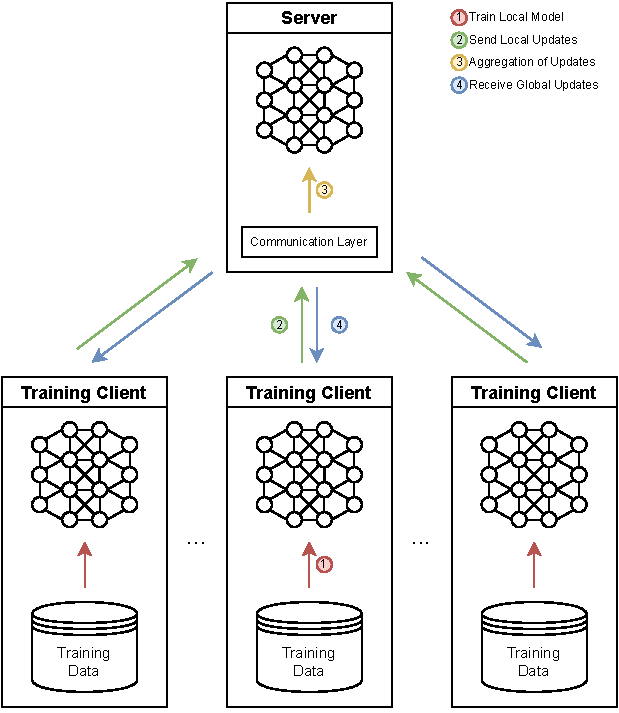
\includegraphics[width=0.6\textwidth]{graphics/hfl-architecture.pdf}
    \caption{Horizontal Federated Learning Architecture}
    \label{fig:hfl_arch}
\end{figure}

\begin{figure}[!hbp]
    \centering
    \centering
    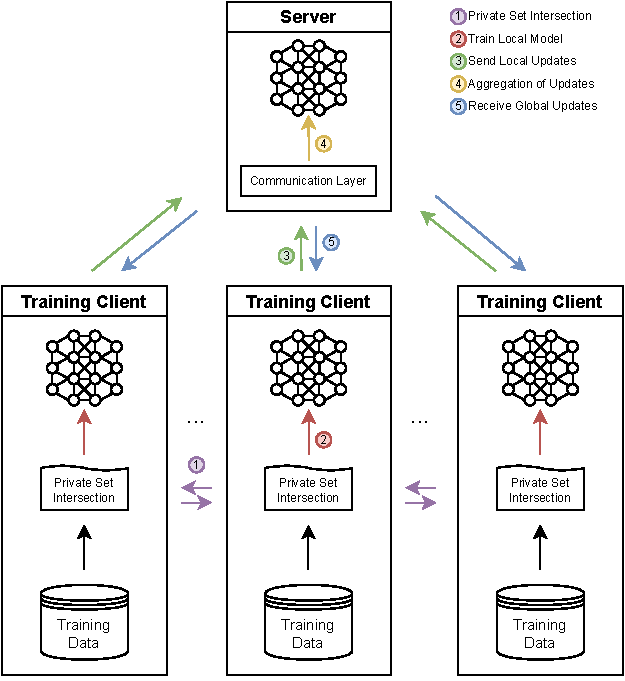
\includegraphics[width=0.6\textwidth]{graphics/vfl-architecture.pdf}
    \caption{Vertical Federated Learning Architecture}
    \label{fig:vfl_arch}
\end{figure}

\section{Blockchain}\label{background:blockchain}

A blockchain is an immutable distributed ledger, which is a database of transactions maintained by several computers, also known as nodes, linked through a peer-to-peer network. The concept of blockchain was first introduced by Stuart Haber and W. Scott Stornetta in 1991 \cite{10.48550/ARXIV.1810.06130}, being popularized by Satoshi Nakamoto in 2008 with the introduction of the cryptocurrency Bitcoin \cite{nakamoto2009bitcoin}.

\begin{figure}[h]
    \centering
    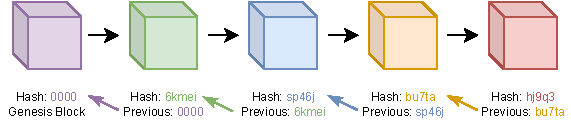
\includegraphics[width=0.8\textwidth]{graphics/blockchain.pdf}
    \caption{Blockchain Representation}
    \label{fig:blockchain_blocks}
\end{figure}

In a blockchain, the data is structured as blocks, as can be seen in \autoref{fig:blockchain_blocks}. Each block contains a certain number of transactions and links to the previous block via a cryptographic hash, forming a chain. This guarantees fidelity and trust without requiring a trusted third party, which is why it is called a \textit{trustless} system. In addition, since the record is immutable and decentralized, all transactions can be transparently viewed by others.

As mentioned beforehand, a blockchain is maintained by several nodes in a peer-to-peer network. As transactions come in, nodes compete in order to generate the next block. Since it is a decentralized process, multiple nodes will try to create the next block of the chain in parallel. In order to reach an agreement between the nodes, a consensus algorithm is used. The consensus algorithm allows to reach an agreement between multiple decentralized nodes without requiring a singular node to be in charge.

\begin{figure}[h]
    \centering
    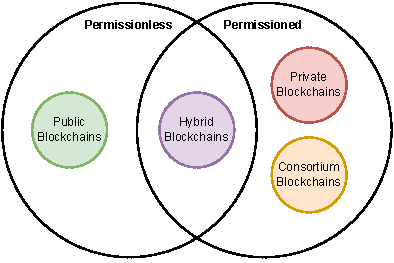
\includegraphics[width=0.5\textwidth]{graphics/blockchain-types.pdf}
    \caption{Blockchain Types}
    \label{fig:blockchain_types}
\end{figure}

\autoref{fig:blockchain_types} illustrates four different types of blockchain, i.e., public, private, consortium, and hybrid. Some are permissionless, which means that anyone can join the network, while some are permissioned, which means that only allowed parties can join the network. 

\begin{itemize}
    \item \textit{Public Blockchains} are permissionless and therefore anyone can join and participate in the network. There is no central authority.

    \item \textit{Private Blockchains}, in contrary to the public blockchains, private blockchains are permissioned with a single central authority. They can only be accessed by allowed parties and they are usually used within organizations.

    \item \textit{Consortium Blockchains}, similarly to the private blockchains, are permissioned. However, instead of being controlled by a single authority, they are controlled by a group of different authorities.

    \item \textit{Hybrid Blockchains} have features of both permissioned and permissionless blockchain systems. They, on one hand, are usually controlled by a single authority, while on the other hand, have a mixed usage of permissioned and permissionless protocols running in parallel for different use cases.
\end{itemize}

\subsection{Smart Contracts}\label{background:smart_contracts}

Smart contracts \cite{8500488} are small computer programs that live within the blockchain and automatically run when predetermined conditions are met. As they live in the blockchain, they are trustless and are typically used to automate the execution of agreements. This way, every party involved in the agreement is certain that it will be honored once the conditions of the agreement are met. Some blockchain platforms, such as Ethereum \cite{wood2014ethereum}, provide functionality for smart contracts.

\subsection{Blockchain Platforms}\label{background:blockchain_platforms}
 
As explained in \autoref{background:blockchain}, blockchain platforms allow developers to build applications on top of the blockchain technologies. Even though all platforms are based on the concept of blockchain, they all have different characteristics and restrictions, as well as different sets of features.

As it can be seen in \autoref{tab:platf_consensus}, around half of the implementations used an already existing platform, where the remaining preferred to implement their own blockchain platform. Among already existing platforms, Ethereum is the most popular. When implementing a custom platform, it is easier to overcome certain restrictions such as limits on data per block \cite{8733825, 9524833}.

\subsection{Consensus Algorithm}\label{background:consensus_algorithms}

The consensus algorithm is one of the most important parts of a Blockchain platform, as it makes it possible for the decentralized blockchain nodes to reach an agreement on what block comes next. Various consensus algorithms can be found in the literature:

\begin{itemize}
    \item The Proof of Work (PoW) consensus algorithm was first introduced in the context of blockchain platforms by Satoshi Nakamoto in Bitcoin \cite{nakamoto2009bitcoin}. It works by means of computation effort proofs, where a set of virtual miners race in solving a complex, yet feasible, mathematical problem. The winner of the race generates a cryptographic proof based on the solution of the problem that can be easily verified by others. Then, the winner adds a new block containing the newly verified transactions to the blockchain. In addition, the winner is rewarded according to some pre-determined rules.
    
    \item The Proof of Authority (PoA) consensus algorithm is a reputation-based consensus algorithm that is most commonly used in private blockchain networks. In this system, there is a set of validator nodes that are responsible for validating the new transactions that stake their own reputation. In addition, the validators are known trusted entities that are manually chosen by the network owner.

    \item The QBFT Byzantine Fault Tolerance (QBFT) \cite{10.48550/arxiv.2002.03613} consensus algorithm is similar to the Practical Byzantine Fault Tolerance (PBFT) algorithm, which is a three-phase protocol that allows a network with $3f+1$ nodes, where $f$ is the maximum amount of faulty nodes, to reach consensus. The different between QBFT and PBFT is that in the former the set of validators is dynamic, while in the latter, it is static. The network reaches a consensus once $2f+1$ nodes agree.
\end{itemize}

\section{Blockchain-based Federated Learning}\label{background:bfl}

Recently, the idea of applying blockchain to FL has emerged. This is motivated by the fact that FL architectures are highly dependent on a single central server, leading to a central point of failure, that can be either overloaded or compromised. With blockchain, the central server can be replaced by multiple decentralized servers that operate the blockchain nodes. In addition, blockchain can provide authentication, traceability, auditability and data preservation.

As stated in \cite{10.48550/arxiv.2110.02182}, so far different types of architectures have been proposed for it, i.e., \textit{Fully Coupled BFL}, \textit{Flexibly Coupled BFL} and \textit{Loosely Coupled BFL}.

\begin{figure}[!ht]
    \centering
    \centering
    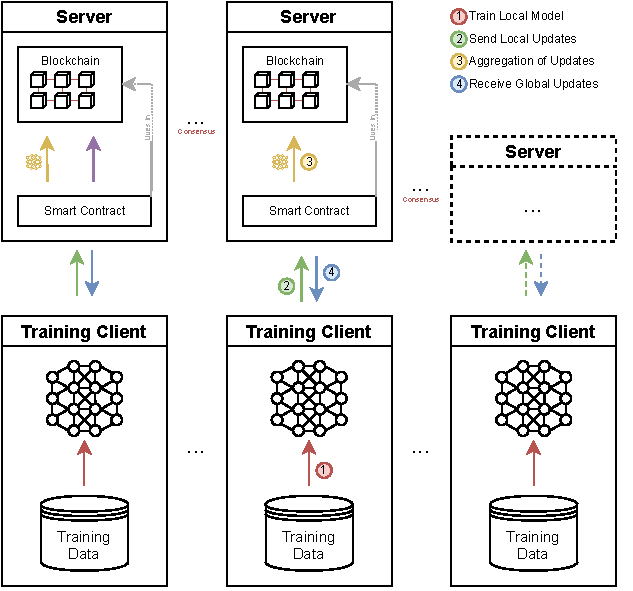
\includegraphics[width=0.6\textwidth]{graphics/bfl-architecture.pdf}
    \caption{Blockchain-based Federated Learning Architecture}
    \label{fig:bfl_arch}
\end{figure}

In a Flexibly Coupled BFL architecture, the blockchain nodes are decoupled from the clients, and run by separate servers. This servers are also responsible for maintaining the blockchain nodes and use the blockchain to store information such as aggregations, scores, among others. The architecture is depicted in \autoref{fig:bfl_arch}.

\subsection{Participants Selection Algorithms}

For the participants selection algorithms, only random selection and first come-first served basis selection will be compared. In the former, both the amount of participants and the participants themselves are selected randomly before the start of each round. In the latter, each participant takes initiative to register for the the next round. Once the limit is reached, no more participants are allowed.

\subsection{Scoring and Aggregation Algorithms}
\label{background:scoring}

Scoring algorithms are used to give each client, or its submission, a score. Based on this score, the submission may have more or less impact on the aggregation, if any at all. In addition, scores are used for reward mechanisms in systems where public models are being trained and clients need some sort of incentive to keep participating \cite{8945913, 8832210, 8905038, 9006344}. In this section, we explain briefly how each of the scoring algorithms that will be compared works and if they influence the aggregation algorithm.

\subsubsection{BlockFlow Score}

The BlockFlow algorithm \cite{10.48550/arxiv.2007.03856} work by giving each submission a score and, based on that score, do the aggregation. In this algorithm, each client $a$ gives each other client $k$ a score $s_{a,k} \in [0.0, 1.0]$, which can be based on $a$'s validation set accuracy using $k$'s submission. Based on this scores, a median score and an evaluation quality scores are calculated. The overall scores will then be the minimum between the scaled median score and the scaled least accurate evaluation score.

With the final scores, the aggregation is calculated using the scores as weights in the Federated Averaging algorithm, instead of the number of samples. More details regarding the algorithm specifics can be found in the original paper.

\subsubsection{Marginal Gain Score}

The Marginal Gain algorithm \cite{10.48550/arxiv.2011.07516}, also known as contributivity score, is calculated by summing the marginal performance gains of all the client's model updates so far. Similarly to BlockFlow scoring, each client has to give each other clients' submission a score. The formula of the client $c$'s submission score $S(c)$ is calculated as follows:

\begin{equation}
    \label{eq:marginal-gain}
    S(c)= \sum_r(v(M_r)-v(M^c_{r+1}))
\end{equation}
, where $v$ is a performance metric, such as accuracy, and $m$ is the model and $r$ the round. These scores are used as weights in the Federated Averaging Algorithm. If the submission's score is equal or below $0$, the submission is ignored.

\subsubsection{Multi-KRUM Score}

The Multi-KRUM algorithm \cite{9170559, Peyvandi2022, 9292450} works by giving each submission a score and eliminating dubious submissions based on their score. This scores are calculated by the servers and are based on the Euclidean distances between the different client $c$'s submissions. The score of each client is denoted as $S(c)$ and calculated as follows:

\begin{equation}
    \label{eq:multi-krum}
    S(c)=\sum_{c \rightarrow k} || \Delta w_c - \Delta w_k|| ^2
\end{equation}

, where $\Delta w$ is a submission and $c \rightarrow k$ are the clients $k$ whose submission $\Delta w_k$ are the $R-f-2$ closest to $\Delta w_c$. In this formula, $R$ is the total number of submissions, while $f$ represents the amount of Byzantine clients. After giving each submission a score, the $R-f$ clients with the lowest scores are chosen and the remaining are rejected. Please note that Byzantine fault tolerant systems behave correctly when no more than $f$ out of $3f+1$ replicas fail.

\section{Differential Privacy}\label{background:diff_priv}

In this thesis, we compare the impact of different degrees of privacy for each scoring algorithm. Even though there are different privacy mechanisms, we will be using Local Differential Privacy. This mechanism is the most used across the literature of the algorithms we will be using and can be applied locally without the need to exchange encryption keys with other clients.

Local Differential Privacy (LDP) is a Differential Privacy technique that ensures a specific degree of privacy. Usually, this is done by using a randomized algorithm $A$ to apply noise to the original data. We say that $A$ provides $\epsilon$-local differential privacy if, and only if, for all subsets $S$ of the image of $A$, and for all pairs of private data $x$ and $x'$:

\begin{equation}
    \label{eq:e-ldp}
    \Pr[A(x) \in S] \leq e^\epsilon \times \Pr[A(x') \in S]
\end{equation}

, where the probability is taken from the randomized algorithm. The lower the $\epsilon$, the higher the degree of privacy.


\chapter{Related Work}\label{chapter:related_work}
In Blockchain-based Federated Learning systems, there are different properties that are need to be taken into consideration when building the system. In this chapter, we go over different properties and what variations are used in the literature.


\section{Consensus Algorithms}
\label{related_work:consensus_algorithms}

One of the most important aspects of blockchain technology is the consensus algorithm. Consensus is the process of reaching an agreement on a single value among different distributed processes. These algorithms are designed to be reliable even on networks that have unreliable nodes. In blockchain, the consensus algorithm is used to reach consensus on the next block of the chain.

\begin{table}[!ht]
\centering
\caption{Consensus Algorithms}
\label{tab:consensus_algorithms}
\begin{tabular}{c|c|c|c|c|c|c|c|c}
\hline \hline
                                    & PoW           & PoA           & PoS           & PoFL          & PoQ           & (p)BFT        & Committee     & Other         \\ \hline \hline
\cite{8905038}                      &               &               &               &               &               &               &               & \checkmark    \\ \hline
\cite{9524833}                      &               &               &               &               &               &               &               & \checkmark    \\ \hline
\cite{9127823}                      &               &               &               & \checkmark    &               &               &               &               \\ \hline
\cite{10.48550/arxiv.2101.03300}    &               &               & \checkmark    &               &               &               &               &               \\ \hline
\cite{9159643}                      &               &               & \checkmark    &               &               &               &               &               \\ \hline
\cite{9223754}                      & \checkmark    &               &               &               &               &               &               &               \\ \hline
\cite{FANG20221}                    &               &               &               &               &               &               &               & \checkmark    \\ \hline
\cite{9399813}                      & \checkmark    &               & \checkmark    &               &               & \checkmark    &               &               \\ \hline
\cite{8832210}                      &               &               &               &               &               &               & \checkmark    &               \\ \hline
\cite{8994206}                      &               &               &               &               &               & \checkmark    &               &               \\ \hline
\cite{8733825}                      & \checkmark    &               &               &               &               &               &               &               \\ \hline
\cite{9274451}                      &               & \checkmark    &               &               &               &               &               &               \\ \hline
\cite{9293091}                      &               &               &               &               &               &               & \checkmark    &               \\ \hline 
\cite{8843900}                      &               &               &               &               & \checkmark    &               &               &               \\ \hline
\cite{8998397}                      &               &               & \checkmark    &               &               &               &               &               \\ \hline
\cite{9311394}                      &               &               & \checkmark    &               &               &               &               &               \\ \hline
\cite{9170905}                      &               &               & \checkmark    &               &               &               &               &               \\ \hline
\cite{8945913}                      &               & \checkmark    &               &               &               &               &               &               \\ \hline
\cite{10.48550/arxiv.2007.03856}    & \checkmark    &               &               &               &               &               &               &               \\ \hline
\cite{10.48550/arxiv.1912.04859}    & \checkmark    &               & \checkmark    &               &               &               &               &               \\ \hline
\cite{9321132}                      &               &               &               &               &               &               & \checkmark    &               \\ \hline
\cite{9079513}                      & \checkmark    &               &               &               &               & \checkmark    &               &               \\ \hline
\cite{app8122663}                   &               &               &               &               &               &               & \checkmark    &               \\ \hline
\cite{9347812}                      &               &               &               & \checkmark    &               &               &               &               \\ \hline
\cite{9134967}                      & \checkmark    &               &               &               &               &               &               &               \\ \hline
\cite{baffle}                       &               & \checkmark    &               &               &               &               &               &               \\ \hline
\cite{9292450}                      &               &               &               & \checkmark    &               &               &               &               \\ \hline
\cite{9210531}                      &               &               &               &               &               &               & \checkmark    &               \\ \hline
\cite{8894364}                      &               &               &               &               &               &               & \checkmark    &               \\ \hline
\cite{10.48550/arxiv.2112.07938}    & \checkmark    &               &               &               &               &               &               &               \\ \hline
\cite{demo}                         &               & \checkmark    &               &               &               &               &               &               \\ \hline
\cite{9233457}                      & \checkmark    &               &               &               &               &               &               &               \\ \hline
\cite{9170559}                      &               &               & \checkmark    &               &               & \checkmark    &               &               \\ \hline
\cite{pirate}                       &               &               &               &               &               &               & \checkmark    &               \\ \hline
\end{tabular}
\end{table}


As can be seen on \autoref{tab:consensus_algorithms}, there is a high variety of consensus algorithms being used among implementations of BFL systems. Below is a summary of each consensus algorithm, as well as some of their characteristics.

\begin{itemize}
    \item \textit{Proof of Work (PoW)} has been used for many years and some of its advantages and disadvantages are now clear. On one hand, it is a simple algorithm where proofs are hard to create, but easy to verify. Not only is it robust and proven to work, but the cost of attacking a PoW blockchain is also extremely high. For an attacker to be successful, they would need to control more than half of the network \cite{li_blockchain_2021}. On the other hand, PoW consumes extreme amounts of energy and it is hard to scale \cite{edwood_2020, li_blockchain_2021, ccaf}. In addition, \cite{10.48550/arxiv.2112.07938} mentions the importance of analyzing the constraints and trade-offs of using PoW with BFL.

    \item \textit{Proof of Stake (PoS)}, in contrast to PoW, does not require high computational resources from the blockchain nodes and therefore the energy consumption can be kept lower. In addition, it allows for fast throughput and nodes are incentivized to behave correctly through the rewarding system \cite{li_blockchain_2021}. On the other hand, some nodes may have excessive influence over the transaction verification process \cite{li_blockchain_2021}. In either case, the details vary from implementation to implementation.
    
    \item \textit{Proof of Authority (PoA)} is a highly sxwcalable consensus algorithm with high throughput \cite{binance_academy_2020}. However, one of the main criticisms of the PoA is that it goes against decentralization since the validators are manually chosen. Therefore, there is hesitation on using PoA in public networks.

    \item \textit{Proof of Federated Learning (PoFL) \cite{9347812, 10.48550/arxiv.2007.15145} and Proof of Quality (PoQ)} \cite{8843900} are both novel consensus algorithms that integrate the training process in order to reduce the resources and energy consumption. These are custom algorithms and they are not readily available on public blockchain platforms. To use it, developers would either need to implement their custom blockchains, or modify an existing blockchain.

    \item \textit{Practical Byzantine Fault Tolerance (PBFT)} allows for high consensus efficiency in high throughput networks \cite{li_blockchain_2021}. However, it will stop working if only 33\% or less nodes are running and it can also have high communication costs due to its three-phase protocol nature.

    \item \textit{Committee-based Consensus} are a group of consensus algorithms where a selected number of members from a committee are selected in order to achieve consensus in a fast way \cite{qu_blockchain-enabled_2022}. This is usually used on custom blockchain implementations with specific goals in mind, such as minimizing communication costs \cite{9293091}.
\end{itemize}

\section{Model Parameter Storage}

Another important aspect of BFL systems is where the model parameters are stored during the training process in order to share them between devices. According to the literature, either the parameters are stored on-chain, i.e., in the blockchain itself, or off-chain, i.e., in a separate storage provider.

\begin{itemize}
    \item With \textit{on-chain storage}, the smart contract stores the model parameters itself \cite{9274451, baffle, demo, 8733825, 9524833, 8894364, 9184854, 8893114}, which means that the parameters themselves will be stored in the blockchain. However, most blockchain platforms have a limit on how large a block can be. Therefore, the amount of data that can be stored per contract is also limited. In these cases, smart contracts are chunked, i.e., a single contract is split into many different contracts that hold smaller chunks of the parameters \cite{9274451, baffle}. In addition, this allows for the new model parameters to be directly calculated through the smart contract as the values are directly accessible.
    
    \item With \textit{off-chain storage}, the smart contract holds a reference to the model parameters in some external storage \cite{10.48550/arxiv.2202.02817, 10.48550/arxiv.1910.12603, 10.48550/arxiv.2007.03856, 8945913, Peyvandi2022, 9170559, 10.1145/3319535.3363256, 10.48550/arxiv.2011.07516}, such a decentralized storage system. In this case, the new model parameters cannot be calculated directly on the smart contract as smart contracts have limited functionality and are not able to download external information during execution. The most common approach is to have a set of devices performing the aggregation in parallel and submitting their final version. Through the smart contract, the majority of the devices must agree on what is the next global version.
\end{itemize}

As can be seen per the list above, most implementations prefer on-chain storage. However, these implementations also use custom blockchain implementations \cite{8733825, 9524833, 8894364, 9184854, 8893114}, which means that they can implement a platform that has different restrictions on how much data a smart contract can handle. When it comes to using already existing blockchain platforms, such as Ethereum, most implementations prefer off-chain storage using a system such as the InterPlanetary File System (IPFS) \cite{10.48550/arxiv.2007.03856, 8945913, Peyvandi2022, 9170559, 10.1145/3319535.3363256, 10.48550/arxiv.2011.07516}.

\section{Participants Selection Techniques}

Usually, only some clients participate in each round. The process of choosing the clients that participate in each round can vary and have different costs. In most cases, the clients were chosen \textit{randomly} \cite{Peyvandi2022}, both the number of clients participating and which clients to participate. In some other systems, clients are allowed to take initiative, operating in a \textit{first come, first served} basis \cite{9184854}. In these systems, a pre-defined number of required clients is set and once enough clients have submitted their updates, the aggregation takes place.

\section{Scoring and Aggregation Techniques}

During the training process, each training client produces their parameter updates and communicates them to the computing devices through the blockchain in order to be aggregated. However, there are different security aspects that should be taken into account here as the parameter updates creates a vector for different attacks, such as poisoning attacks and plagiarism attacks.

\begin{itemize}
    \item \textit{Poisoning attacks} happen when training clients willingly send parameter updates that decrease the quality of the model. They may have been generated using an honestly unreliable data set, or done on purpose. To avoid other participants to provide unreliable data in order to degrate the model performance, there are dynamic verification technniques that allow to ignore low quality data \cite{10.48550/arxiv.2110.02182, 10.48550/arxiv.2104.10501}.
    
    \item \textit{Plagiarism attacks} happen when lazy clients plagiarize other client's models updates without real training \cite{9403374}, which can be addressed via pseudo-noise techniques \cite{10.48550/arxiv.2009.09338}.
\end{itemize}

Most of the current literature focus on poisoning attacks, as they can affect the most the final model performance. In addition, plagiarism attacks within the same round can be avoided by secure communication methods, such as differential privacy; and plagiarism attacks where a node reuses parameters from a previous round can be avoided by simply hashing the parameter values and performing a comparison. It is important to notice that different verification techniques directly affect the security model of the system \cite{10.48550/arxiv.2110.02182}. There are different solutions found in the literature regarding verification:

\begin{itemize}
    \item \textit{Integrated Consensus Techniques}. Some authors implement their own blockchain systems, which allows them to design their own consensus algorithm dedicated to Federated Learning. This consensus techniques can use properties from the training process directly in order to detect which updates to accept or reject \cite{9293091, 10.1007/978-981-15-9213-3_12}.
    
    \item \textit{Random Committee}. In some works, a random set of participants is selected as committee and they must vote whether or not the model updates should be accepted. The decision to accept is based on the amount of votes that each submission received \cite{9159643}. There are different algorithms to decide on how voting works, such as voting in favor or against depending if it increases the performance relatively to the previous model or not.
    
    \item \textit{Points-based System}. Points-based system, also known as reputation-based system, usually work by giving clients with consistently high quality data and updates higher amounts of points. Then, the updates with less points are either rejected, or they have a smaller influence on the aggregation  \cite{10.48550/arxiv.2011.07516, 9170559, Peyvandi2022, 9292450}.
    
    \item \cite{8945913} implements a novel verification technique based on the trend of the validation error accuracy. To implement this, the updates by each training device are validated using a public validation data set known to all devices. The result of this validation will also influence the reward distribution.

\end{itemize}

The costs of model update scoring have not been considered in most of the literature and it is important to understand the trade-off between system costs and the different scoring techniques \cite{9403374, 10.48550/arxiv.2110.02182}.

\section{Privacy Techniques}

\todo{Mention the existing ones (diff privacy, homomorphic encryption, etc) and cite}

\section{Conclusions}

From the literature review, we can take a few conclusions. Firstly, there is a clear lack on how different BFL properties, such as consensus algorithms and scoring techniques, impact communication and computation costs and accuracy. The survey \cite{9403374} also noticed this. Therefore, this work intends to fill such gap by providing a detailed analysis on how some of this properties influence the accuracy, communication and computation costs.

Secondly, even though there are many works on designing BFL frameworks, very few are released to the public, or are modular. On this work, we will work on designing and implementing a modular BFL framework that can be easily changed to support other techniques and will be available to the public to empower future research.  


\chapter{Framework Design and Implementation}\label{chapter:framework}
In this chapter, we provide detailed information regarding the design of our modular framework, as well as its implementation.

\section{Blockchain Platform}

In this work, we focus on already existing blockchain platforms that do not require internal changes to make the system work. The Ethereum is our platform of choice as it is the most popular and compatible with all the techniques we use for our experiments and comparison with the related work.

\section{Architecture}

Even though the modular framework we build in this work is capable of operating in different architectures, we focus on what is called Flexibly Coupled BFL.

\section{BlockLearning Framework's Design}\label{framework:design}

The modular framework, to which we called BlockLearning, is designed in such a way that modules can be added, as well as removed or changed, easily. In this framework, the devices, identified by the address of their account in the blockchain, can be classified into three categories: \textit{trainers}, \textit{aggregators} and \textit{scorers}. Additionally, the entity that deploys the contract and is responsible for starting and terminating the rounds is called \textit{owner}.

A device can be categorized as one or more categories. By doing so, the framework provides flexibility to support different architectures and algorithms. For example, BlockFlow's scoring algorithm is done at the clients, which are then categorized as trainers and scorers, while the servers are categorized as aggregators. In contrast, Multi-KRUM is executed at the servers, which are then categorized as aggregators and scorers, while the clients are categorized as trainers.

% The following sections present the execution flow of the framework, as well as the structure and modules of BlockLearning.

% \section{Execution Flow}\label{meth:exec_flow}

\begin{figure}[!ht]
    \centering
    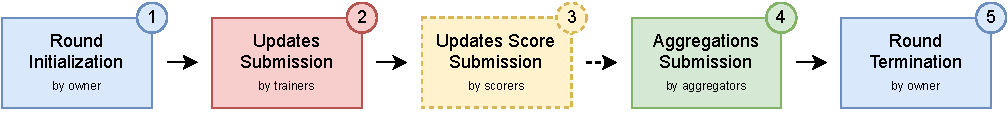
\includegraphics[width=1\textwidth]{graphics/sequence.pdf}
    \caption{BlockLearning Flow}
    \label{fig:blocklearning_steps}
\end{figure}

The framework supports a modular sequential flow represented in \autoref{fig:blocklearning_steps}. The steps are explained below:

\begin{enumerate}
    \item In first place, the owner initializes the round. During the round initialization, depending on the participant selection algorithm, the trainers that will participate may have been selected already, or not.
    
    \item In second place, the trainers retrieve the information such as the global weights from the last round and train the model using their local data. Then, the trainers submit their model updates.
    
    \item In third place, if a scoring algorithm is enabled, the scorers retrieve the updates and calculate the scores. Then, they submit their scores.
    
    \item In fourth place, the aggregators retrieve the model updates and execute the aggregation algorithm and submit the aggregation results.
    
    \item In fifth place, if we are using vertically partitioned data, and depending on the model in use, the trainers may have to confirm back-propagation. Note that this step is tightly connected to the model we will be using for Vertical Federated Learning, which will be introduced later. Nonetheless, it shows how modular the system can be and how steps can be easily added at different points of the flow for different purposes.
    
    \item Finally, the round is marked as terminated by the owner. At this point, the smart contract decides which is the final aggregation for the model based on the submissions by the aggregators.
\end{enumerate}

\subsection{Threat Model}

In the last step of the execution flow, the smart contract decides the final aggregation values based on the submissions by the aggregators. For this, at least 50\% of the aggregators must agree on the same aggregation in order for it to be accepted. Therefore, the framework offers a 50\% threat model.

Even though 50\% is not the ideal threat model, it is an improvement compared to classic FL, in which the central aggregator is a central point of failure that needs to be available, reliable, and trusted at all times. In this framework, an attacker would have to control over 51\% of the servers in order to be able to influence the outcome of the aggregation, and therefore, or the training.

In addition, the framework should allow for the threat threshold to be changed. By default, it is 50\%. However, if a user prefers that all aggregators must agree on the same aggregation, they should be able to do so.

\subsection{Structure and Modules}\label{meth:struct_modules}

The framework is divided into three main components: the smart contracts, the library, and the testbed. These are depicted on \autoref{fig:blocklearning_modules} and will be individually explained on the following subsections.

\begin{figure}[!ht]
    \centering
    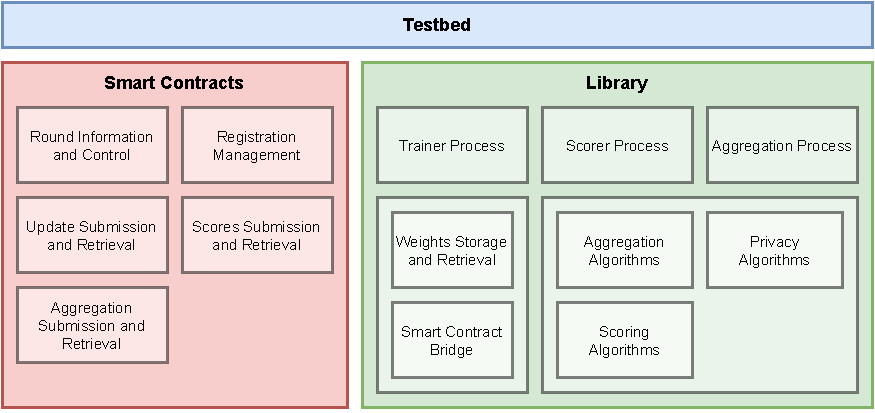
\includegraphics[width=1\textwidth]{graphics/modules.pdf}
    \caption{BlockLearning's  Structure and Modules}
    \label{fig:blocklearning_modules}
\end{figure}

\subsubsection{Smart Contracts}\label{meth:smart_contracts}

The first component of the framework is the smart contracts. The smart contracts live on the blockchain and are the main means of communication between FL clients and servers. In addition, the smart contracts hold information regarding the current status of the round, as well as the updates, scores, aggregations, among others. The smart contracts provide the following functionality:

\begin{itemize}
    \item \textit{Round Information and Control}: the smart contract must provide information on whether the round is ongoing and which phase, i.e., scoring, aggregation, or termination phase, it is in. It must allow for flexibility such that new phases can be added in the future. In addition, it must allow for rounds to be started and marked as terminated. Round phase advancements are defined through pre-defined conditions that, once met, automatically move the round to the next phase. For example, after all updates are received, the smart contract should move to the next phase.
    
    \item \textit{Registration Management}: the smart contract must allow devices to register themselves as trainers, aggregators, or scorers in the system. Regarding the owner, it is automatically assigned to whom deployed the contract. Finally, it should provide information about which devices participate in each round.
    
    \item \textit{Update Submission and Retrieval}: the smart contract must allow trainers to submit their updates, which must include a pointer to the model weights and the amount of data points that were used to train the model. In addition, it can include the training accuracy and testing accuracy for each individual trainer. The submissions must be accessible.
    
    \item \textit{Scores Submission and Retrieval}: the smart contract must allow scorers to submit their scores. It must be possible to know which scorer scored which update and they must be accessible.
    
    \item \textit{Aggregation Submission and Retrieval}: the smart contract must allow aggregators to submit the aggregations, which contain a pointer to the weights. The aggregations must be accessible.
\end{itemize}

\subsubsection{Library}\label{meth:library}

The second component of the framework is the library. The library encodes the algorithms, utilities, and building blocks necessary to implement the process that runs on the clients and the servers. It must include:

\begin{itemize}
    \item \textit{Aggregation, Scoring} and \textit{Privacy Algorithms}: for which a common interface must be implemented, such that adding new algorithms is easy and simple and they are interchangeable in the code.
    
    \item \textit{Weights Storage and Retrieval}: utilities to load and store weights on the decentralized storage provider. These must also provide an interface in order to make it easy to change the storage provider by providing a different implementation.
    
    \item \textit{Smart Contract Bridge}: a contract class that provides an interface to the smart contract that lives on the blockchain. With this class, it should be possible to call the smart contract functions as if they were local functions.
    
    \item \textit{Trainer, Scorer} and \textit{Aggregator Classes}: a class per each device category. This class must register the devices as their category upon initialization. It must also provide methods to execute the training, scoring and aggregation tasks, respectively.
\end{itemize}

\subsubsection{Testbed}\label{meth:testbed}

The third component of the framework is the testbed. The testbed provides the platform to conduct the experiments in a reproducible way. It must include:

\begin{itemize}
    \item \textit{Client} and \textit{Server Processes}: scripts that will be run at the clients and the servers, respectively. These scripts will use the library in order to perform the right tasks according to which algorithm is being used.
    
    \item \textit{Federated Learning Setup and Deployment}: scripts and tools to easily deploy the client and server machines in a test environment, such as containers.
    
    \item \textit{Blockchain Setup and Deployment}: scripts and tools to easily deploy the blockchain network in a test environment, as well as deploy the contract to such network.
\end{itemize}

In addition, the testbed must also include tools to collect the required statistics and logs that can be later processed to retrieve the previously discussed metrics.

\section{BlockLearning Framework's Implementation}

In this section, we go over the implementation details of the BlockLearning framework, following the guidelines defined in \Cref{framework:design}. The complete implementation is publicly available on GitHub\footnote{\url{https://github.com/hacdias/blocklearning}}.

\subsection{Smart Contracts}

As mentioned previously, this work uses the Ethereum \cite{wood2014ethereum} blockchain platform. Therefore, the smart contracts must be implemented in a programming language that supports Ethereum. We chose the Solidity \cite{solidity} programming language as it is the most well-known with the widest support.

Since our framework supports different algorithms with different requirements, we implemented four different smart contracts. These smart contracts inherit most of their functionality from an abstract smart contract that provides the common data structures and functionality, named \texttt{Base}. Then, we implement the following classes, that derive from \texttt{Base}:

\begin{itemize}
    \item \texttt{NoScoring}, which is used when we do not need a scoring algorithm. It only adds a new function to the \texttt{Base} class in order to allow the owner to start a round.
    
    \item \texttt{Scoring}, which is used when we need a scoring algorithm. This smart contract implements the required methods to support the scoring phase, such as scoring submissions and the scoring round.
    
    \item \texttt{FirstComeFirstServed}, which is used with the first-come first-served participant selection algorithm. It overrides some of the \texttt{Base} functions in order to register participants to the round as they submit their updates.
    
    \item \texttt{Vertical}, which is used with vertically partitioned data, specifically with the Split-CNN. It incorporates the functionality required to provide for an additional phase, the backpropagation, as well as more information about the head and top models.
\end{itemize}

A class diagram with the public interfaces of the contracts, as well as the data types, is depicted in \autoref{fig:contracts-uml}.

\begin{figure}[!ht]
    \centering
    \centering
    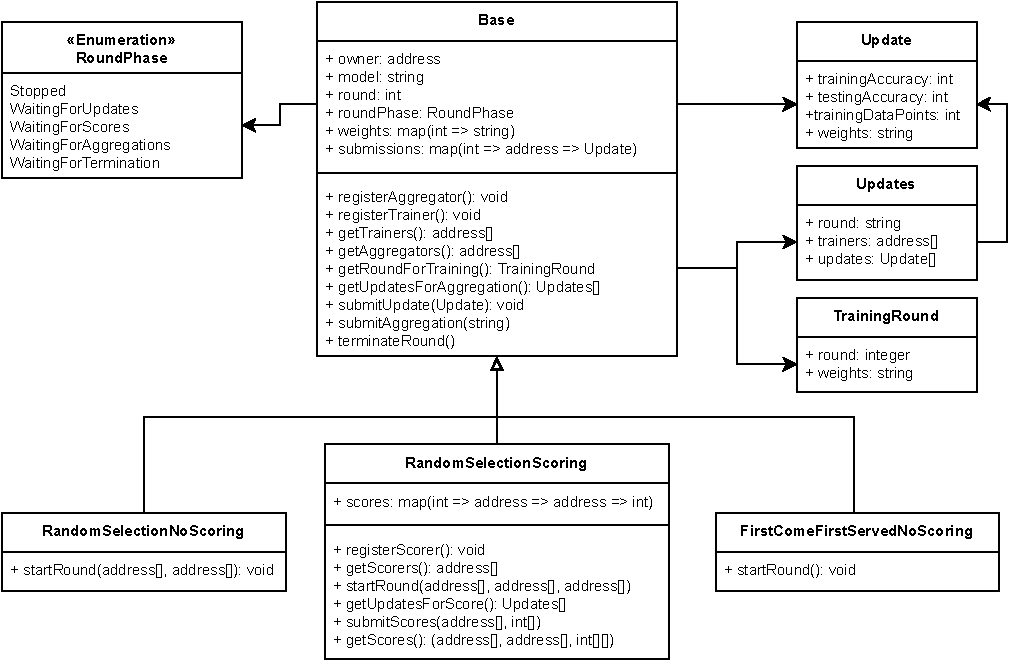
\includegraphics[width=1\textwidth]{graphics/smart-contract-uml.pdf}
    \caption{Smart Contracts Class Diagram}
    \label{fig:contracts-uml}
\end{figure}

An interesting aspect to note is that score and accuracy values are stored as integers. Currently, Solidity does not support floating point numbers. To preserve fidelity, the original values are multiplied by a large integer, $10^{18}$. Then, when the values are retrieved from the smart contract, they are divided by the same value in order to get the original value.

\subsection{Library}

The library is implemented in the Python \cite{10.5555/1593511} programming language. The main motivation for using Python is that many well-known Machine Learning libraries, such as TensorFlow \cite{tensorflow2015-whitepaper} and PyTorch \cite{NEURIPS2019_9015} are implemented in Python, as well as many data processing tools.

The first part of the library is the aggregation, scoring and privacy algorithms. Each of these categories of algorithms has a specific interface to which each algorithm must conform to. By having a common interface, we can implement new algorithms, or change existing ones, easily. The interfaces are as follows:

\begin{itemize}
    \item \texttt{aggregate(trainers, updates, scorers, scores) $\rightarrow$ weights}\\
    The aggregators must provide a function \texttt{aggregate} that receives an array with the trainer addresses, an array with the updates sorted by the same order as the trainers, an array with the scorers and an array with the scores sorted by the same order as the scorers. It is important to note that the scorers and the scores are optional arguments since a scoring algorithm is not always required. The function returns an array with the aggregated weights. % BlockFlow, FedAvg, Multi-KRUM
    
    \item \texttt{score(round, trainers, updates) $\rightarrow$ trainers, scores}\\
    The scorers must provide a function \texttt{score} that receives an integer with the round number, an array with the trainer addresses, as well as an array of updates that are sorted by the same order as the trainer addresses. The function returns an array with the trainers and their submission scores. % Multi-KRUM, MarginalGain, Accuracy (BlockFlow)
    
    \item \texttt{privatize(x) $\rightarrow$ y}\\
    The privacy mechanisms must provide a function \texttt{score} that receives an array of the weights \texttt{x} and returns the privatized weights \texttt{y}. % Gaussian
\end{itemize}

The second part of the library is the utilities to store and retrieve the weights, as well as the smart contract bridge. The weights storage class also provides a common interface such that it is possible to change which storage provider we use. As for our experiments, we use IPFS, explained in \Cref{background:ipfs}, similarly to many other works. The smart contract bridge is a class that creates a 1:1 connection with the functions from the smart contracts.

The third and final part of the library is the \texttt{Trainer}, \texttt{Scorer} and \texttt{Aggregator} classes. These classes implement the main flow of each of these procedures using the modules aforementioned described. For example, the trainer class is initialized with the contract bridge, the weights storage, the model, the data and an optional privacy mechanism. Then, it provides a method \texttt{train()} that executes the training procedure. Similarly, the scorer class provides \texttt{score()} and the aggregator class provides \texttt{aggregate()}.

\subsection{Testbed}

The testbed, that is, the platform to conduct the experiments. It was mostly implemented using the aforementioned library and Docker \cite{docker}. Docker is a platform that allows to easily deploy applications in an isolated setting through what is called a container, allowing us to simulate multiple devices in the same network. Each container runs an image, which is the name given to the piece of software than runs on the container.

In the testbed, we have two major components: the client, server and owner scripts, the federated learning environment deployment and the blockchain deployment. These are discussed on the following subsections.

\subsubsection{Client, Server and Owner Scripts}

The client, server and owner scripts are the processes that will run at the client, server and owner, respectively. These are implemented using the BlockLearning library. In each of these scripts, we first load the required data, such as the data set in the clients, and initialize the required algorithms, namely the scoring, aggregation and privacy algorithms.

Then, depending on the scoring algorithm, we initialize the relevant classes at the correct machines. For example, for the BlockFlow scoring algorithm, the client initializes a \texttt{Trainer} and a \texttt{Scorer}, while the server initializes an \texttt{Aggregator}. In contrast, for Multi-KRUM, the client only initializes a \texttt{Trainer}, while the server initializes an \texttt{Aggregator} and a \texttt{Scorer}. On \autoref{alg:client_loop} you can visualize part of the main loop of the client script.

\begin{algorithm}
\caption{Client Script Main Loop}\label{alg:client_loop}
\begin{algorithmic}
\Require $s \in$ \{\O, BlockFlow, MarginalGain\}
\State $T \gets $ Initialize Trainer
\If{$s$ is not \O}
    \State $S \gets $ Initialize Scorer
\EndIf
\While{True}
    \State $P \gets$ Get Phase From Smart Contract
    \If{$P$ is Waiting For Updates}
        \State Execute Training Procedure $T$
    \ElsIf{$P$ is Waiting For Scores}
        \State Execute Scoring Procedure $S$
    \EndIf
\EndWhile
\end{algorithmic}
\end{algorithm}

\subsubsection{Blockchain Setup and Deployment}

The Blockchain setup and deployment is done using already existing tools and our library. As previously mentioned, we use Docker containers in order to run the experiments. Moreover, we use Docker Compose in order to deploy multiple containers at once and orchestrate the deployment process.

We use different Ethereum implementations, depending on the consensus algorithm since they are not all available within the sample implementation. Ethereum's main implementation, \texttt{go-ethereum} \cite{go-ethereum}, provides PoA and PoW. For QBFT, we use a fork called \texttt{quorum}\cite{quorum}, which is mostly identical to \texttt{go-ethereum} but supports QBFT.

Moreover, the Blockchain setup and deployment follows the following steps:

\begin{enumerate}
    \item \textit{Generate Accounts}. In first place, the Ethereum accounts for the clients and servers are generated using the provided \texttt{go-ethereum} toolkit. Each account is pre-loaded with $100$ ETH, the Ethereum currency, so that clients or servers will not run out of currency to submit their transactions.
    
    \item \textit{Build Images}. In second place, we build the Docker images that will be used to deploy the Blockchain network. This images are based on the images provided by each of the Ethereum's implementations that we use. In addition, they pre-load the account information, as well as some additional configuration to ensure that all nodes are connected when the network is bootstrapped.
    
    \item \textit{Deploy Network}. In third place, the network is deployed using Docker Compose and the configured amount of nodes.
    
    \item \textit{Deploy Contract}. Finally, the contract is deployed to the network using Truffle, which is a tool designed to help developers developing and deploying smart contracts.
\end{enumerate}

Finally, we would like to mention that originally we were planning on testing the PoS consensus algorithm too. However, the only fork providing PoS support does not work in private network settings\footnote{\url{https://github.com/bnb-chain/bsc/issues/861}}. Therefore, it was not possible to run an experiment with PoS.

\subsubsection{Federated Learning Setup and Deployment}

Similarly to the Blockchain setup and deployment, we also use Docker Compose for the Federated Learning system. The process is identical as in the previous section, except that we only build the images and deploy the Federated Learning network.

\section{Model Parameter Storage}\label{background:ipfs}

For this work, we will be using an off-chain model parameter storage, namely the InterPlanetary File System (IPFS). IPFS \cite{10.48550/arxiv.1407.3561} is a decentralized storage system and protocol used by many of the works reviewed in \Cref{chapter:related_work} to store the model parameters and other relevant information that would otherwise be too large to be on the blockchain.

IPFS is a content addressed file system, which implies that, every file is addressed by its content. It works by attributing a hash, based on the file's content. Using this hash, also known as Content Identifier (CID), the file can be retrieved from the network and guaranteed to be immutable. Instead of storing the entire file in the blockchain, the CID can be stored. Pairing IPFS with the blockchain keeps the system decentralized and distributed, while offloading the storage to a different system.

\chapter{Experimental Setup and Evaluation}\label{chapter:evaluation}
In this chapter, we provide information on the evaluation of the experiments described in the previous chapters. Below, we indicate which data set is used, how it is partitioned, which models are used, among other details. In the end, we provide an overview of all of the executed experiments, compared to the literature.

\section{Data Set}

The data set used for the experiments is the MNIST\cite{lecun2010mnist} data set. The MNIST data set includes 70 000 images of handwritten digits from 0 to 9, where each image is 28 by 28 pixels. Some samples can be visualized in \autoref{fig:mnist}.

\begin{figure}[!htp]
    \centering
    \centering
    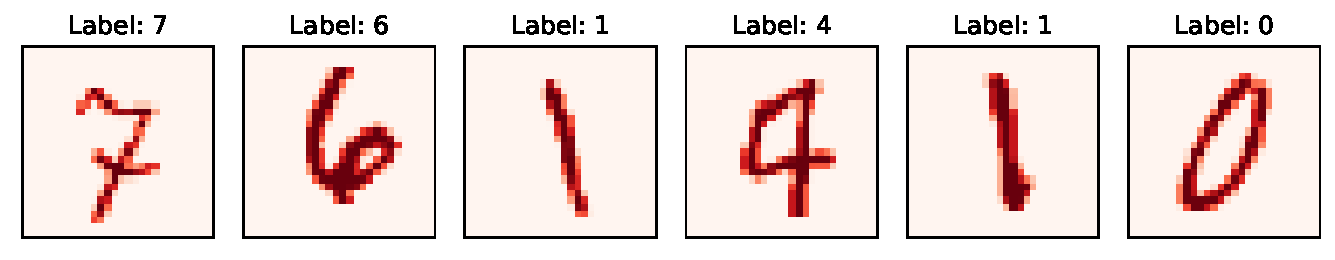
\includegraphics[width=1\textwidth]{graphics/mnist.pdf}
    \caption{MNIST Example Samples}
    \label{fig:mnist}
\end{figure}

Not only is it a widely known data set, but also used by the majority of the reviewed works, as can be seen in \autoref{tab:data_distribution}. Since we will compare our accuracy with the original works in order to validate our results, we need to ensure that the configurations are as similar as possible.

\section{Data Partitioning}

In this section, we show the horizontal and vertical data partitioning according to the methods described in \Cref{chapter:methodology}. To divide the data horizontally, we used a publicly available tool\footnote{\url{https://github.com/TsingZ0/PFL-Non-IID}} that supports partitioning the MNIST data set directly using the Dirichlet distribution. We did so for 5, 10, 25 and 50 clients.

On \autoref{fig:horizontal_dist}, you can visualize the \textit{non-iid} horizontal partitioning for 10 clients. It is possible to see how \textit{non-iid} the distribution is, both in terms of samples amount and in terms of class distribution. For example, client 7 has many samples from classes 2 and 4, while having none of the remaining classes. At the same time, client 10 has a few samples from classes 0, 1, 2 and 9 and many from class 7.

\begin{figure}[!ht]
    \centering
    \centering
    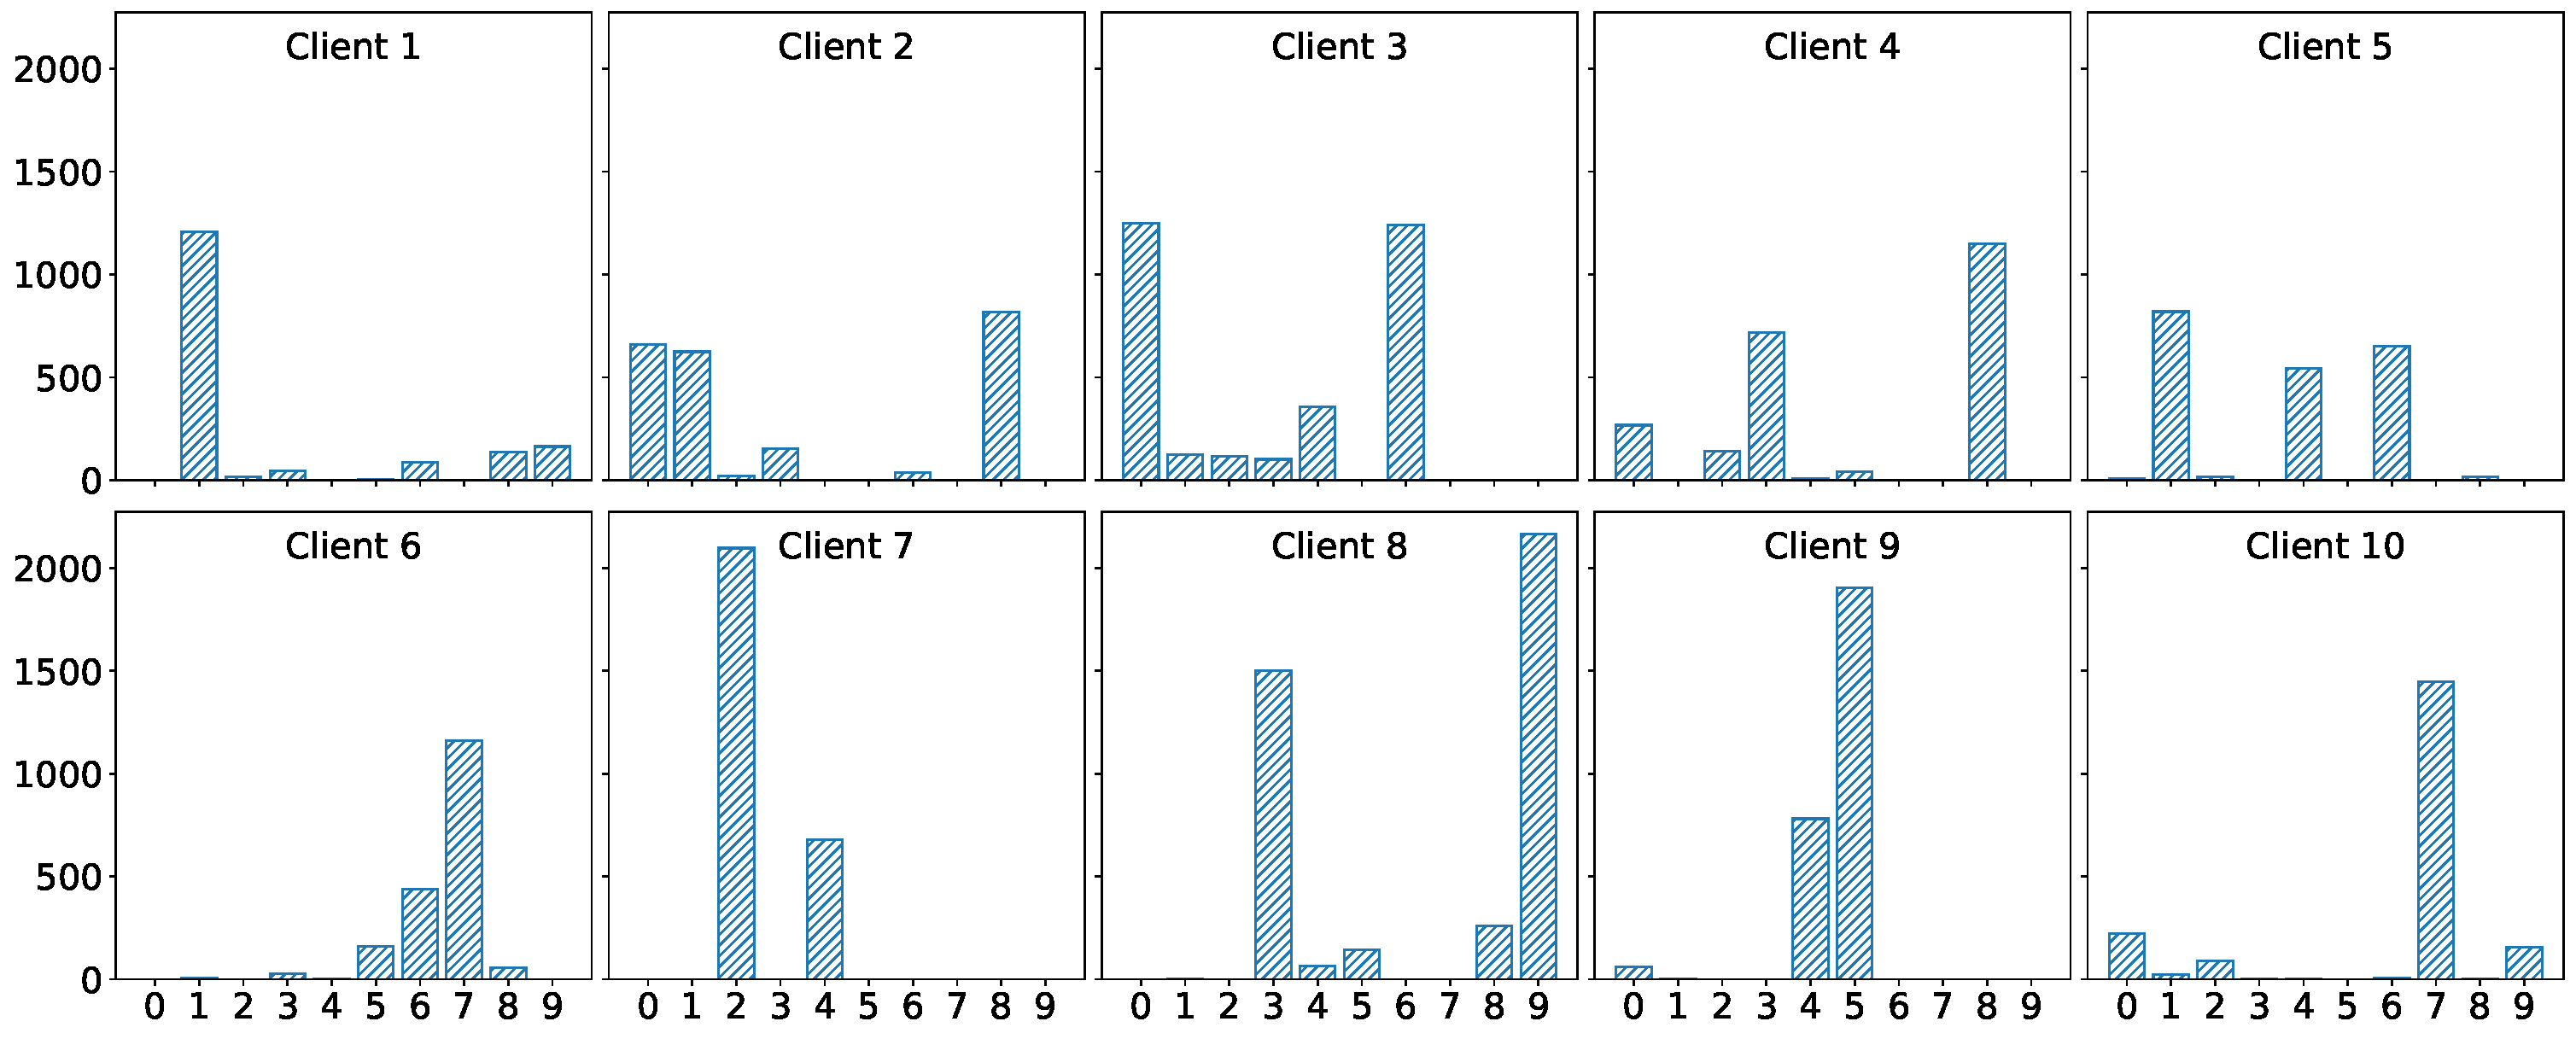
\includegraphics[width=1\textwidth]{graphics/10_dist.pdf}
    \caption{Horizontal Data Distribution For 10 Clients}
    \label{fig:horizontal_dist}
\end{figure}

Regarding vertically partitioning data, it was mentioned in \Cref{subsection:verticalpartitioning} that more details would be provided in the present chapter. The vertical data partitioning highly depends on both the model and the data set. For this experiment, we will use a Split-CNN which will be introduced in the next section. To use such model, the owner is expected to have the labels, while the clients are expected to some features of each sample. In the case of the MNIST data set, we can think of the features as vertical segments of the image. To divide a 28 by 28 image sample between 2 clients, for example, we split the image into two 14 by 28 segments, as depicted in \autoref{fig:vertical_dist}.

\begin{figure}[!ht]
    \centering
    \centering
    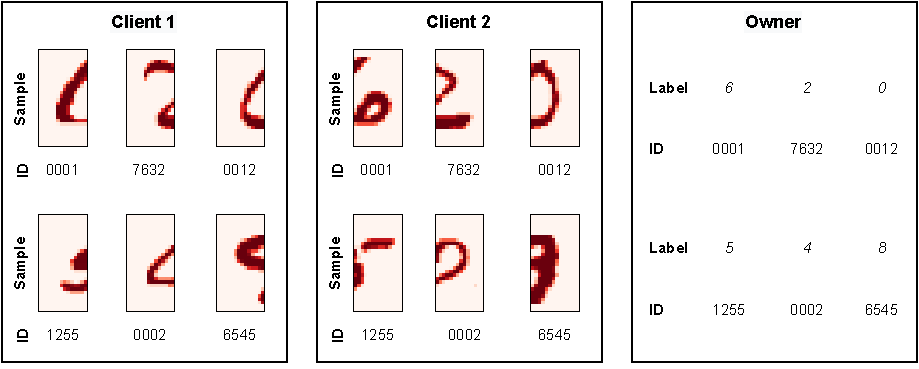
\includegraphics[width=1\textwidth]{graphics/vertical_partitioning.pdf}
    \caption{Vertical Data Distribution for 2 Clients}
    \label{fig:vertical_dist}
\end{figure}

\section{Machine Learning Models}

The models used on this work are simple models based on previous literature. The goal of this work is not to provide the most efficient, or accurate, model. Therefore, we do not dive into the details of the models. The models used for horizontal and vertical training are succinctly explained below.

For horizontal training, we use a simple Convolutional Neural Network (CNN) with three levels of convolution intercalated with max pooling to reduce overfitting. These layers are followed by a flattening layer and two dense layers that culminate in the output. The layer details can be seen in \autoref{tab:cnn}.

\begin{table}[!h]
    \begin{tabular}{c|c}
        \hline \hline
        Layer Type       & Output Shape \\ \hline \hline
        Convolutional 2D & (26, 26, 32) \\ \hline
        Max Pooling 2D   & (13, 13, 32) \\ \hline
        Convolutional 2D & (11, 11, 64) \\ \hline
        Max Pooling 2D   & (5, 5, 64)   \\ \hline
        Convolutional 2D & (3, 3, 64)   \\ \hline
        Flatten          & (576)        \\ \hline
        Dense            & (64)         \\ \hline
        Dense            & (10)         \\ \hline
    \end{tabular}
    \caption{CNN Model}
    \label{tab:cnn}
\end{table}

For vertical training, we use a dual-headed, or four-headed, Split-CNN \cite{10.1145/3297858.3304038, 10.48550/arxiv.2104.00489}, depending on whether we have two, or four, clients. The model at the clients is the head model, while the model at the servers is the tail model. To train this model, each client gives their input data to the models and collects the output of the last layer. Then, this intermediate output is sent to the servers, which are then given to the tail model. The servers calculate the gradients, which are then backpropagated to the clients. For more details, please consult the original works where the workings of this model are given in more detail. On \autoref{tab:splitnn} you can see the details of the dual-headed Split-CNN model.

\begin{table}[!h]
    \begin{subtable}[h]{0.49\textwidth}
        \centering
        \begin{tabular}{c|c}
            \hline \hline
            Layer Type       & Output Shape \\ \hline \hline
            Convolutional 2D & (26, 12, 32) \\ \hline
            Max Pooling 2D   & (13, 6, 32) \\ \hline
            Convolutional 2D & (11, 11, 64) \\ \hline
            Max Pooling 2D   & (5, 2, 64)   \\ \hline
        \end{tabular}
        \caption{Head}
    \end{subtable}
    \hfill
    \begin{subtable}[h]{0.49\textwidth}
        \centering
        \begin{tabular}{c|c}
            \hline\hline
            Layer Type     & Output Shape \\ \hline\hline
            2 Input Layers & (5, 2, 64)   \\ \hline
            Concatenation  & (5, 2, 128)  \\ \hline
            Flatten        & (1280)       \\ \hline
            Dense          & (512)        \\ \hline
            Dense          & (256)        \\ \hline
            Dense          & (10)         \\ \hline
        \end{tabular}
        \caption{Tail}
     \end{subtable}
     \caption{Split-CNN Dual-Headed Model}
     \label{tab:splitnn}
\end{table}

\section{Hardware and Software Specifications}

The experiments were executed in a remote machine whose hardware and software specifications can be found in \autoref{tab:temps}. Due to resource limitations, it was not possible to have a machine with GPU. Furthermore, if we consider that FL systems are being run in IoT clients, it is unlikely that such low-powered devices would have a GPU available. In addition, the MNIST data set and the models in use are relatively simple, which means that they can be easily trained using a CPU. Nonetheless, it is worth mentioning that the training process would be faster in machines with a GPU.

\begin{table}[!h]
    \begin{subtable}[h]{0.59\textwidth}
        \centering
        \begin{tabular}{l|l} \hline \hline
            Hardware & Model                                    \\ \hline \hline
            CPU      & AMD Ryzen 5 3600 6-Core 4.2 GHz          \\ \hline
            RAM      & 64 GB                                    \\ \hline
            Disk     & 500 GB NVMe                              \\ \hline
        \end{tabular}
        \caption{Hardware}
        \label{evaluation:hardware}
    \end{subtable}
    \hfill
    \begin{subtable}[h]{0.39\textwidth}
        \centering
        \begin{tabular}{l|l} \hline \hline
            Software            & Version               \\ \hline \hline
            Docker              & 20.10.15              \\ \hline
            Docker Compose      & 2.5.0                 \\ \hline
            Python              & 3.8.13               \\ \hline
            Node.js             & 16.15.0               \\ \hline
            Truffle             & 5.5.13               \\ \hline
            Ganache             & 7.1.0               \\ \hline
            Solidity            & 0.5.16               \\ \hline
        \end{tabular}
        \caption{Software}
        \label{evaluation:software}
     \end{subtable}
     \caption{Hardware and Software Specifications}
     \label{tab:temps}
\end{table}

\section{Results}

\autoref{tab:experiments} presents a summary of all of our experiments, as well as other works. On it, it is possible to see the configuration of all of the experiments that were executed. Due to space limitations, not all information is presented on the table. All experiments use the MNIST data set, except for the works \cite{10.48550/arxiv.2007.03856, 10.48550/arxiv.2011.07516} whose data set is unknown. In addition, all the experiments were executed with 50 rounds, except for \cite{9170559} which is also unknown. We can see that our results, in terms of accuracy, are within the range of the original works of the scoring algorithms. Therefore, we can validate our results.

The detailed analysis of the results of each experiment are presented in the following chapters. \Cref{chapter:analysis:consensus_algorithms} presents the analysis on the consensus algorithms experiments. \Cref{fig:participations_client} analyzes the results on the participant selection algorithms experiments. \Cref{chapter:analysis:scoring} presents the analysis on the scoring algorithms experiments. \Cref{chapter:analysis:clients} analyzes the results on the impact of the number of clients. \Cref{chapter:analysis:privacy} presents the results and analysis of the impact of different privacy degrees. Finally, \Cref{chapter:vertical} presents the results of the Proof of Concept of Vertical Federated Learning applied in a Blockchain-based Federated Learning environment.

\begin{landscape}

\begin{table}[]
\begin{tabular}{c|c|c|c|c|c|c|c|c|c|c} \hline \hline
\multirow{2}{*}{Group}                                                                      & \multirow{2}{*}{ID} & \multirow{2}{*}{Work}                     & Consensus                  & \multirow{2}{*}{Clients} & Participants            & Scoring                        & \multicolumn{2}{c}{Data}                & Privacy                & \multirow{2}{*}{Accuracy}              \\ 
                                                                                            &                     &                                            & Algorithms                 &                          & Selection     &                       & P          & D       & Degree                 &                                        \\ \hline \hline
\multirow{3}{*}{\begin{tabular}[c]{@{}c@{}}Consensus\\ Algorithms\end{tabular}}             & 1                   & \multirow{3}{*}{$\star$}                         & PoA                        & \multirow{3}{*}{25}      & \multirow{3}{*}{Random} & \multirow{3}{*}{None}          & \multirow{3}{*}{H} & \multirow{3}{*}{N} & \multirow{3}{*}{None}  & 98.54                                  \\ \cline{2-2}\cline{4-4}\cline{11-11}
                                                                                            & 2                   &                                            & PoW                        &                          &                         &                                &                    &                    &                        & 98.35                                  \\ \cline{2-2}\cline{4-4}\cline{11-11}
                                                                                            & 3                   &                                            & IBFT                       &                          &                         &                                &                    &                    &                        & 98.90                                  \\\hline
\multirow{2}{*}{\begin{tabular}[c]{@{}c@{}}Participant Selection\\ Techniques\end{tabular}} & 1                   & \multirow{2}{*}{$\star$}                         & \multirow{2}{*}{PoA}       & \multirow{2}{*}{25}      & Random                  & \multirow{2}{*}{None}          & \multirow{2}{*}{H} & \multirow{2}{*}{N} & \multirow{2}{*}{None}  & 98.54                                  \\ \cline{2-2}\cline{6-6}\cline{11-11}
                                                                                            & 4                   &                                            &                            &                          & F.C.F.S &                                &                    &                    &                        & 98.18                                  \\ \hline
\multirow{4}{*}{\begin{tabular}[c]{@{}c@{}}Scoring\\ Techniques\end{tabular}}               & 1                   & \multirow{4}{*}{$\star$}                         & \multirow{4}{*}{PoA}       & \multirow{4}{*}{25}      & \multirow{4}{*}{Random} & None                           & \multirow{4}{*}{H} & \multirow{4}{*}{N} & \multirow{4}{*}{None}  & 98.54                                  \\
                                                                                            & 10                  &                                            &                            &                          &                         & BlockFlow                      &                    &                    &                        & 97.04                                  \\
                                                                                            & 14                  &                                            &                            &                          &                         & Marginal Gain                  &                    &                    &                        & 98.58                                  \\
                                                                                            & 18                  &                                            &                            &                          &                         & Multi-KRUM                     &                    &                    &                        & 97.00                                  \\ \hline
\multirow{21}{*}{\begin{tabular}[c]{@{}c@{}}Number\\ of Clients\end{tabular}}               & 5                   & \multirow{4}{*}{$\star$}                         & \multirow{4}{*}{PoA}       & 5                        & \multirow{4}{*}{Random} & \multirow{4}{*}{None}          & \multirow{4}{*}{H} & \multirow{4}{*}{N} & \multirow{4}{*}{None}  & 97.76                                  \\
                                                                                            & 6                   &                                            &                            & 10                       &                         &                                &                    &                    &                        & 97.06                                  \\
                                                                                            & 1                   &                                            &                            & 25                       &                         &                                &                    &                    &                        & 98.54                                  \\
                                                                                            & 7                   &                                            &                            & 50                       &                         &                                &                    &                    &                        & 98.88                                  \\ \hline
                                                                                            & 8                   & \multirow{4}{*}{$\star$}                         & \multirow{4}{*}{PoA}       & 5                        & \multirow{4}{*}{Random} & \multirow{4}{*}{BlockFlow}     & \multirow{4}{*}{H} & \multirow{4}{*}{N} & \multirow{4}{*}{None}  & 97.94                                  \\
                                                                                            & 9                   &                                            &                            & 10                       &                         &                                &                    &                    &                        & 85.92                                  \\
                                                                                            & 10                  &                                            &                            & 25                       &                         &                                &                    &                    &                        & 97.04                                  \\
                                                                                            & 11                  &                                            &                            & 50                       &                         &                                &                    &                    &                        & 97.84                                  \\ \hline
                                                                                            & \multirow{3}{*}{}   & \multirow{3}{*}{\cite{10.48550/arxiv.2007.03856}} & \multirow{3}{*}{PoW}       & 25                       & \multirow{3}{*}{?}      & \multirow{3}{*}{BlockFlow}     & \multirow{3}{*}{H} & \multirow{3}{*}{?} & \multirow{3}{*}{$\epsilon =$ ?} & \multirow{3}{*}{$\geq$ 85.00} \\
                                                                                            &                     &                                            &                            & 50                       &                         &                                &                    &                    &                        &                                        \\
                                                                                            &                     &                                            &                            & 100                      &                         &                                &                    &                    &                        &                                        \\ \hline
                                                                                            & 12                  & \multirow{4}{*}{$\star$}                         & \multirow{4}{*}{PoA}       & 5                        & \multirow{4}{*}{Random} & \multirow{4}{*}{Marginal Gain} & \multirow{4}{*}{H} & \multirow{4}{*}{N} & \multirow{4}{*}{None}  & 89.12                                  \\
                                                                                            & 13                  &                                            &                            & 10                       &                         &                                &                    &                    &                        & 96.62                                  \\
                                                                                            & 14                  &                                            &                            & 25                       &                         &                                &                    &                    &                        & 98.58                                  \\
                                                                                            & 15                  &                                            &                            & 50                       &                         &                                &                    &                    &                        & 98.90                                  \\ \hline
                                                                                            &                     & \cite{10.48550/arxiv.2011.07516}                  & ?                          & ?                        & ?                       & Marginal Gain                  &                    & ?                  & None                   & $\geq$ 90.00                  \\ \hline
                                                                                            & 16                  & \multirow{4}{*}{$\star$}                         & \multirow{4}{*}{PoA}       & 5                        & \multirow{4}{*}{Random} & \multirow{4}{*}{Multi-KRUM}    & \multirow{4}{*}{H} & \multirow{4}{*}{N} & \multirow{4}{*}{None}  & 96.68                                  \\
                                                                                            & 17                  &                                            &                            & 10                       &                         &                                &                    &                    &                        & 98.44                                  \\
                                                                                            & 18                  &                                            &                            & 25                       &                         &                                &                    &                    &                        & 97.00                                  \\
                                                                                            & 19                  &                                            &                            & 50                       &                         &                                &                    &                    &                        & 98.48                                  \\
                                                                                            &                     & \cite{9170559}                                    & PoS, pBFT                  &                          & ?                       &                                &                    & I                  & $\epsilon =$ 10                 & 98.00                                  \\
\multirow{18}{*}{\begin{tabular}[c]{@{}c@{}}Privacy\\ Degrees\end{tabular}}                 & 1                   & \multirow{3}{*}{$\star$}                         & \multirow{3}{*}{PoA}       & \multirow{3}{*}{25}      & \multirow{3}{*}{Random} & \multirow{3}{*}{None}          & \multirow{3}{*}{H} & \multirow{3}{*}{N} & None                   & 98.54                                  \\
                                                                                            & 19                  &                                            &                            &                          &                         &                                &                    &                    & $\epsilon =$ 5                  & 98.18                                  \\
                                                                                            & 20                  &                                            &                            &                          &                         &                                &                    &                    & $\epsilon =$ 1                  & 80.22                                  \\
                                                                                            & 10                  & \multirow{3}{*}{$\star$}                         & \multirow{3}{*}{PoA}       & \multirow{3}{*}{25}      & \multirow{3}{*}{Random} & \multirow{3}{*}{BlockFlow}     & \multirow{3}{*}{H} & \multirow{3}{*}{N} & None                   & 97.04                                  \\
                                                                                            & 21                  &                                            &                            &                          &                         &                                &                    &                    & $\epsilon =$ 5                  & 94.00                                  \\
                                                                                            & 22                  &                                            &                            &                          &                         &                                &                    &                    & $\epsilon =$ 1                  & 84.68                                  \\
                                                                                            &                     & \cite{10.48550/arxiv.2007.03856}                  & PoW                        & 25                       & ?                       & BlockFlow                      & H                  & ?                  & $\epsilon =$ ?                  & $\geq$ 85.00                  \\
                                                                                            & 14                  & \multirow{3}{*}{$\star$}                         & \multirow{3}{*}{PoA}       & \multirow{3}{*}{25}      & \multirow{3}{*}{Random} & \multirow{3}{*}{Marginal Gain} & \multirow{3}{*}{H} & \multirow{3}{*}{N} & None                   & 98.58                                  \\
                                                                                            & 23                  &                                            &                            &                          &                         &                                &                    &                    & $\epsilon =$ 5                  & 98.36                                  \\
                                                                                            & 24                  &                                            &                            &                          &                         &                                &                    &                    & $\epsilon =$ 1                  & 92.26                                  \\
                                                                                            &                     & \cite{10.48550/arxiv.2011.07516}                  & ?                          & ?                        & ?                       & Marginal Gain                  &                    & ?                  & None                   & $\geq$ 90.00                  \\
                                                                                            & 18                  & \multirow{3}{*}{$\star$}                         & \multirow{3}{*}{PoA}       & \multirow{3}{*}{25}      & \multirow{3}{*}{Random} & \multirow{3}{*}{Multi-KRUM}    & \multirow{3}{*}{H} & \multirow{3}{*}{N} & None                   & 97.00                                  \\
                                                                                            & 25                  &                                            &                            &                          &                         &                                &                    &                    & $\epsilon =$ 5                  & 94.70                                  \\
                                                                                            & 26                  &                                            &                            &                          &                         &                                &                    &                    & $\epsilon =$ 1                  & 91.00                                  \\
                                                                                            &                     & \cite{Peyvandi2022}                               & ?                          & \multirow{4}{*}{?}       & Random                  & \multirow{4}{*}{Multi-KRUM}    &                    & N                  & $\epsilon =$ ?                  & 94.39                                  \\
                                                                                            &                     & \multirow{3}{*}{9170559}                   & \multirow{3}{*}{PoS, pBFT} &                          & \multirow{3}{*}{?}      &                                & \multirow{3}{*}{}  & \multirow{3}{*}{I} & $\epsilon =$ 10                 & 98.00                                  \\
                                                                                            &                     &                                            &                            &                          &                         &                                &                    &                    & $\epsilon =$ 5                  & 96.50                                  \\
                                                                                            &                     &                                            &                            &                          &                         &                                &                    &                    & $\epsilon =$ 1                  & 86.00                                  \\
\multirow{2}{*}{\begin{tabular}[c]{@{}c@{}}Vertical Federated\\ Learning\end{tabular}}      & 27                  & \multirow{2}{*}{$\star$}                         & \multirow{2}{*}{PoA}       & 2                        & \multirow{2}{*}{N/A}    & \multirow{2}{*}{N/A}           & \multirow{2}{*}{V} & \multirow{2}{*}{N} & \multirow{2}{*}{None}  &                                        \\
                                                                                            & 28                  &                                            &                            & 4                        &                         &                                &                    &                    &                        &                                       
\end{tabular}
\end{table}

\end{landscape}

\chapter{Impact Analysis of Consensus Algorithms}\label{chapter:analysis:consensus_algorithms}
In this chapter, we analyze the first experiment, that is, the impact of using different consensus algorithms in a Blockchain-based Federated Learning system. In this set of experiments, all properties of the system are static, except for the consensus algorithm, which vary between PoA, PoW and QBFT.

\section{Time and Transactions}

The first interesting statistics we look into are the E2E time, the mean time it takes for a round to complete, as well as the mean transaction latency and the mean transaction cost. These are represented in \autoref{tab:metrics_consensus_algorithms}.

\begin{table}[!ht]
\centering
\begin{tabular}{c|c|c|c} \hline \hline
Metric                              & PoA    & PoW    & QBFT   \\ \hline \hline
E2E Time (m)            & 18.93  & 30.62  & 18.97  \\ \hline
Mean Round Time (s)             & 22.70  & 36.72  & 22.74  \\ \hline
% Median Time Per Round (s)           & 21.90  & 35.28  & 21.99  \\ \hline \hline
Mean Transaction Latency (s)    & 1.549  & 1.821  & 1.558  \\ \hline
% Median Latency Per Transaction (s)  & 1.549  & 1.554  & 1.555  \\ \hline \hline
Mean Transaction Cost (Gas)     & 183124 & 227052 & 182880 \\ \hline
% Median Cost Per Transaction (Gas)   & 185198 & 229866 & 185068 \\ \hline \hline
\end{tabular}
\caption{Time, Transaction Latency and Transaction Costs Per Consensus Algorithm}
\label{tab:metrics_consensus_algorithms}
\end{table}

Regarding time, we can observe that different consensus algorithms can lead to very different running times. On one hand, PoA and QBFT are the fastest consensus algorithms, providing the lowest E2E times and mean round times. Additionally, the difference between both is minimal, differing only $0.04$ seconds per round. On the other hand, PoW takes the longest, being $1.6$ times slower than both PoA and QBFT.

Transaction latency and costs follow a similar trend as the running times. Both PoA and QBFT have similar transaction latency and cost, differing in a small amount, while PoW has a higher transaction latency and cost. When compared, PoW costs $1.2$ times more than using PoA and QBFT.

As explained in \autoref{background:consensus_algorithms}, PoW works by solving increasingly complex mathematical puzzles that consume high amounts of resources. This intense process can lead to slower response rates, which translates to higher transaction latency and costs. This, in turn, increases the time it takes for each round to complete.

\section{Accuracy}

Regarding accuracy, as can be seen in \autoref{fig:accuracy_consensus_algorithms}, it does not change significantly with different consensus algorithms. Consensus algorithms dictate the order at which the transactions are processed and ensures consistency between the multiple blockchain nodes. This only affects the blockchain inner workings, and not the ML process. Therefore, it was not expected that the consensus algorithms would have an impact on the accuracy.

\begin{figure}[!ht]
    \centering
    \centering
    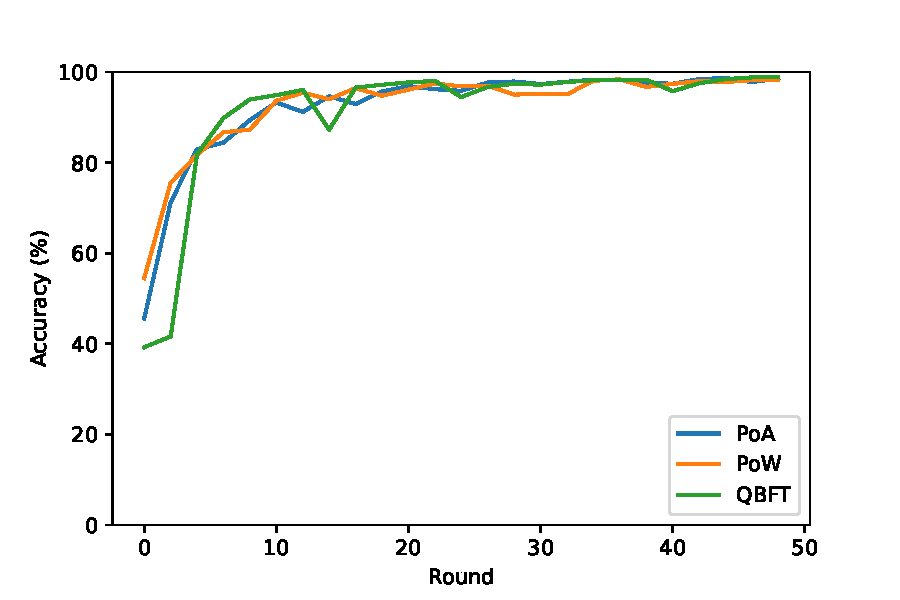
\includegraphics[width=0.7\textwidth]{graphics/01_consensus_accuracy.pdf}
    \caption{Accuracy Per Consensus Algorithm}
    \label{fig:accuracy_consensus_algorithms}
\end{figure}

\section{Communication Costs}

For the communication costs, we analyze the inbound and outbound network traffic per round at the training clients, computing servers and blockchain nodes. This values can be observed in \autoref{fig:net_consensus_algorithms}.

On one hand, the inbound and outbound traffic for the clients and server has negligible differences when using different consensus algorithms. As mentioned in the previous section, the consensus algorithms have no expected impact on the ML process. Since the clients and servers only concern the ML process, it was expected that the clients and servers would not be affected. The small differences we can observe, in the order of $< 2$ MB, are likely connected to fluctuations in the random participant selection mechanism. If there are more participants being selected, more data needs to be transmitted, and vice-versa.

On the other hand, the traffic at the blockchain nodes varies considerably depending on the consensus algorithm. On average, PoW requires more bandwidth per round than PoA, but the difference is very minimal. However, QBFT requires $2$ times more network traffic than PoW and $4$ times more traffic than PoA. QBFT is a three-phase consensus algorithm, which requires a higher amount of network messages to be transmitted before reaching consensus. In addition, the size of the messages also differs. When combining both of this aspects, we can conclude that the expected network traffic per round using the QBFT algorithm would be higher.

\begin{figure}[!ht]
    \centering
    \centering
    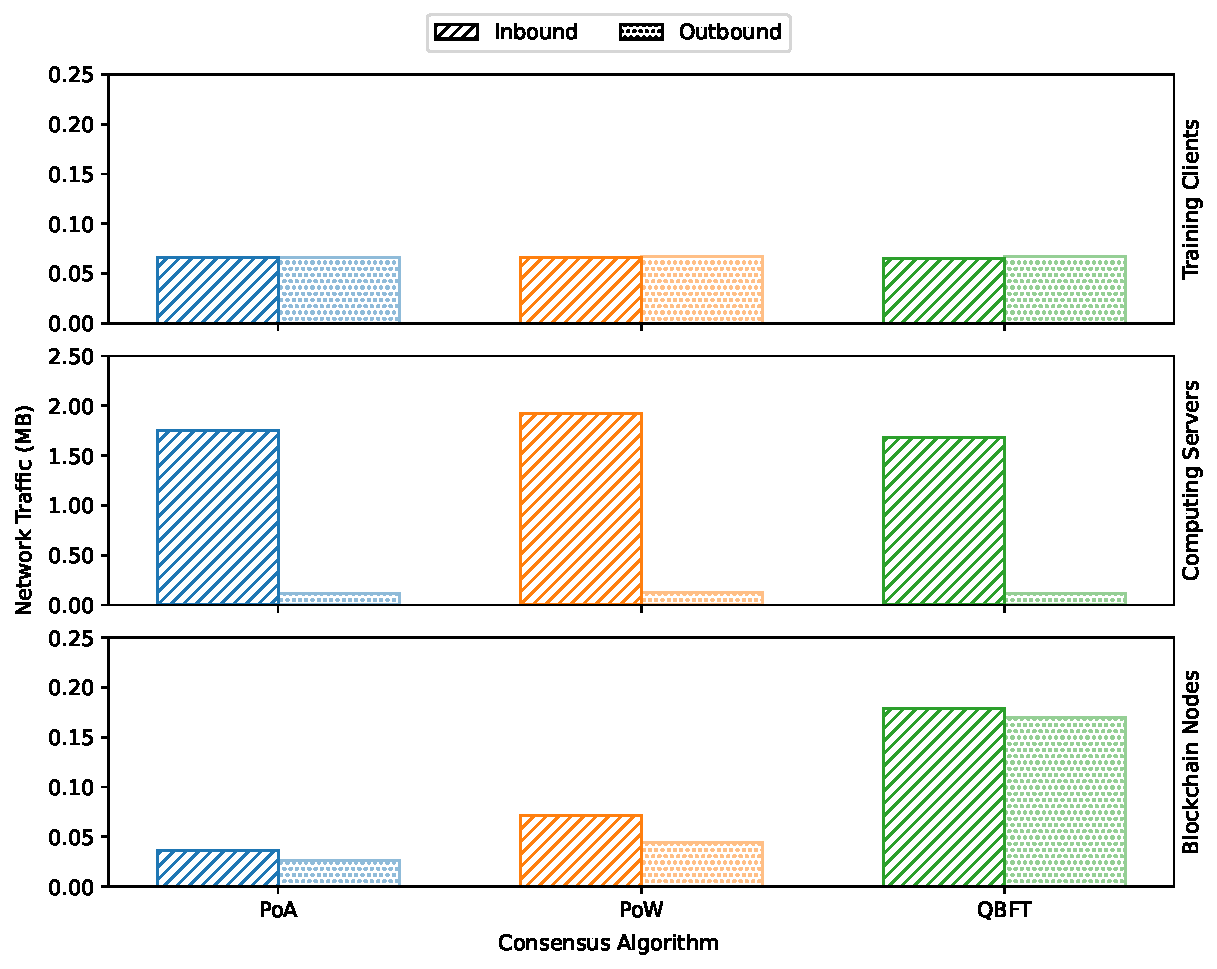
\includegraphics[width=0.8\textwidth]{graphics/01_consensus_net.pdf}
    \caption{Network Traffic Per Round Per Consensus Algorithm}
    \label{fig:net_consensus_algorithms}
\end{figure}

\section{Computation Costs}

Regarding computation costs, we will look at both RAM and CPU usage on the training clients, computing servers and blockchain nodes. To do so, we have \autoref{fig:ram_consensus_algorithms} and \autoref{fig:cpu_consensus_algorithms}, that show the mean RAM usage and mean CPU usage, respectively, per consensus algorithm during the execution of the experiments. As mentioned previously, the execution times for PoA and QBFT are lower than for PoW, which can be seen in the figures by not having more data past minute 19. Additionally, as explained before, the consensus algorithms are not expected to have a direct impact on the clients or the servers.

\begin{figure}[!hpt]
    \centering
    \centering
    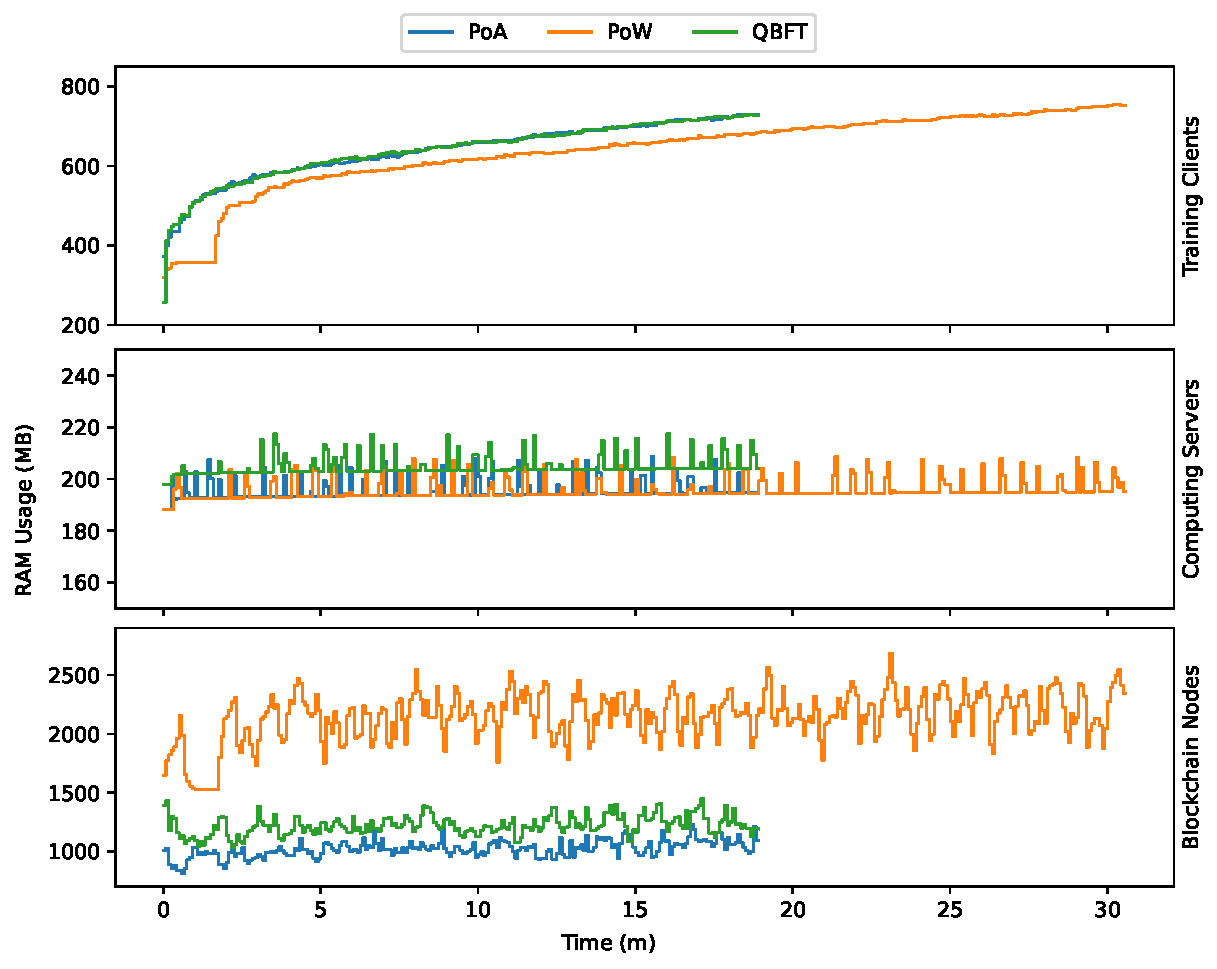
\includegraphics[width=0.8\textwidth]{graphics/01_consensus_ram.pdf}
    \caption{RAM Usage Per Consensus Algorithm}
    \label{fig:ram_consensus_algorithms}
\end{figure}

\begin{figure}[!hpb]
    \centering
    \centering
    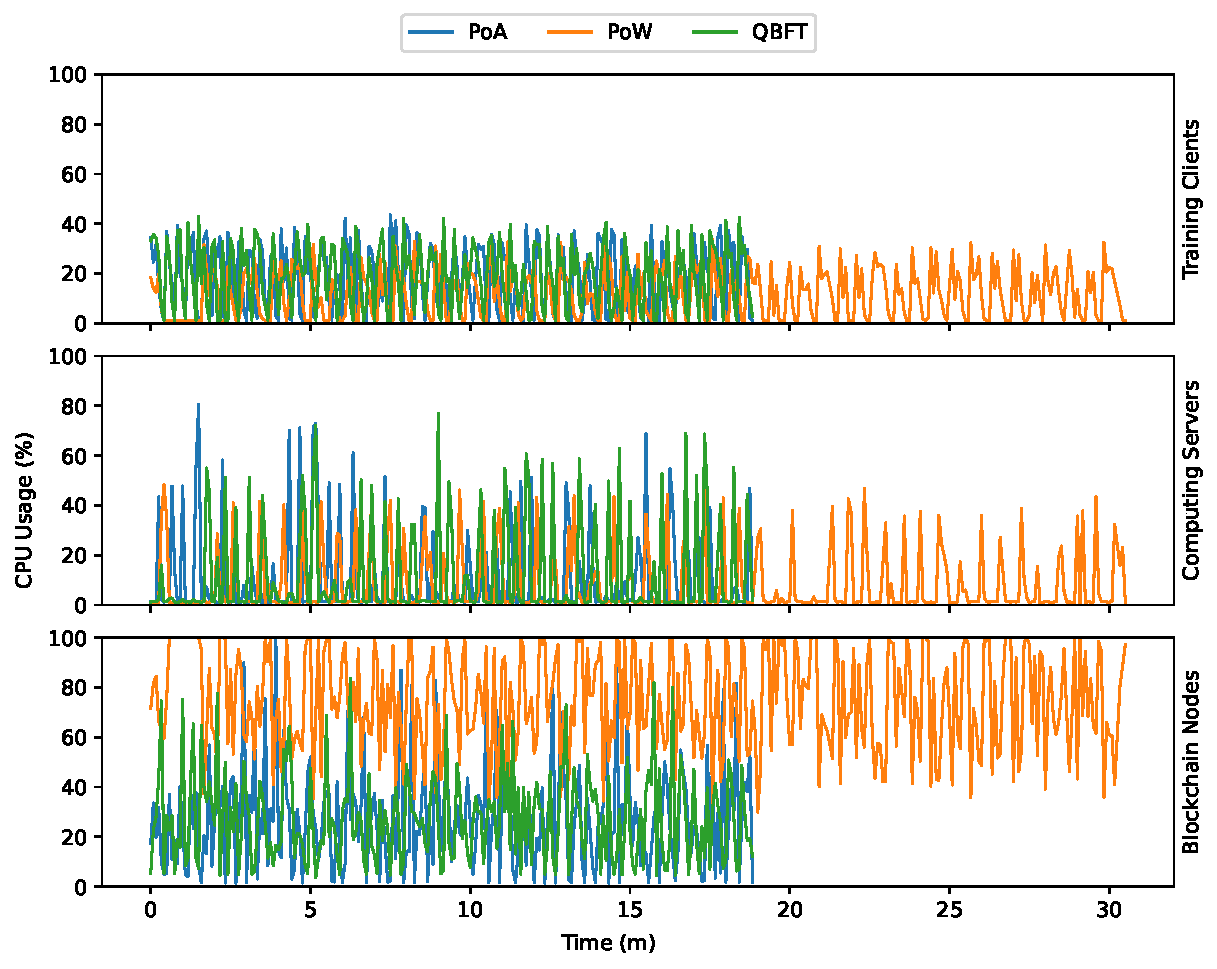
\includegraphics[width=0.8\textwidth]{graphics/01_consensus_cpu.pdf}
    \caption{CPU Usage Per Consensus Algorithm}
    \label{fig:cpu_consensus_algorithms}
\end{figure}

Regarding the clients, the RAM usage and CPU usage do not differ significantly regardless of which consensus algorithm is used. On one hand, we have the RAM usage, where we can observe that the clients reach the same peak. However, the rate at which that peak is reached is different. For PoW, since there are higher transaction latencies, it takes longer to reach the next round, leading to a slower growing RAM usage during the training. On the other hand, we have the CPU usage, where we can observe that there are more idle moments, that is, moments at which the CPU usage is lower. This can also be explained by the higher transaction latencies, during which the clients cannot do anything other than wait.

Regarding the servers, the same reasoning as for the clients can be applied. On one hand, the RAM usage is consistent across different consensus algorithms. We can, however, notice that when using QBFT, the RAM usage at the servers is slightly higher. However, this is a likely negligible difference, as the difference is minimal ($< 10$ MB) considering the total RAM Usage ($\approx 200$ MB). On the other hand, the CPU usage is similar to what we observed for the clients, with a higher amount of idle moments.

Regarding the blockchain nodes, we can visualize a larger difference, both in RAM usage and CPU usage. For both, PoW consumes a much higher level of resources. On average, PoW consumes $2$ times more then RAM and has a $2$ times higher CPU usage. This can also be explained by the way PoW works by solving complex mathematical puzzles, which require intense computation resources.

\section{Conclusions}

In conclusion, we can observe that different consensus algorithms have no direct impact on the accuracy and computation and communication costs at the clients and servers. However, it has an impact on the time and computation and communication costs at the blockchain servers. PoA and QBFT are much faster than PoW. In addition, they require less computation power, both in RAM and CPU. However, QBFT consumes incurs more communication costs than both PoA and PoW. Therefore, there is a clear correlation between the computation costs and the time it takes. The higher the communication costs, the higher the transaction latencies, which translates to slower round times.

Assuming the blockchain network is only being used for Federated Learning, PoA is the most cost-effective of the consensus algorithms we analyzed. In case the network network is needed for other applications, other properties might be required to be taken into account.

For future work, it would be interesting to see if the Ethereum blockchain could be adapted to easily incorporate the custom consensus mechanisms that were seen in \ref{related_work:consensus_algorithms}. These algorithms work by producing proofs directly from the Machine Learning process. That can lead to better usage of resources if the blockchain network is solely used for a Federated Learning system.

\chapter{Impact Analysis of Horizontal Federated Learning}\label{chapter:horizontal}
In this chapter, we analyze the impact of using different participant selection and scoring algorithms on a Blockchain-based Federated Learning (BFS) system with horizontal data partition. In addition, for each scoring algorithm, we analyze how they behave and how the system is impacted by different number of clients, as well as privacy degrees. Due to the high number of plots, the communication and computation costs plots are placed in \Cref{chapter:horizontal_appendix}.

\section{Participant Selection Algorithms}

In this set of experiments, all properties of the system are static, except for the participant selection algorithm, which can be either random selection or first-come first-served.

Both algorithms choose the number of clients in the same way, via a uniform random distribution. However, the clients themselves are chosen differently. Consequently, it is possible that the distribution of chosen clients is slightly different, which may affect the system performance. \autoref{fig:participations_client} illustrates client participation (represented by the bars), as well as the average number of participation per client (represented by the lines). It is clear from the plot that the distributions are different.

\begin{figure}[!ht]
    \centering
    \centering
    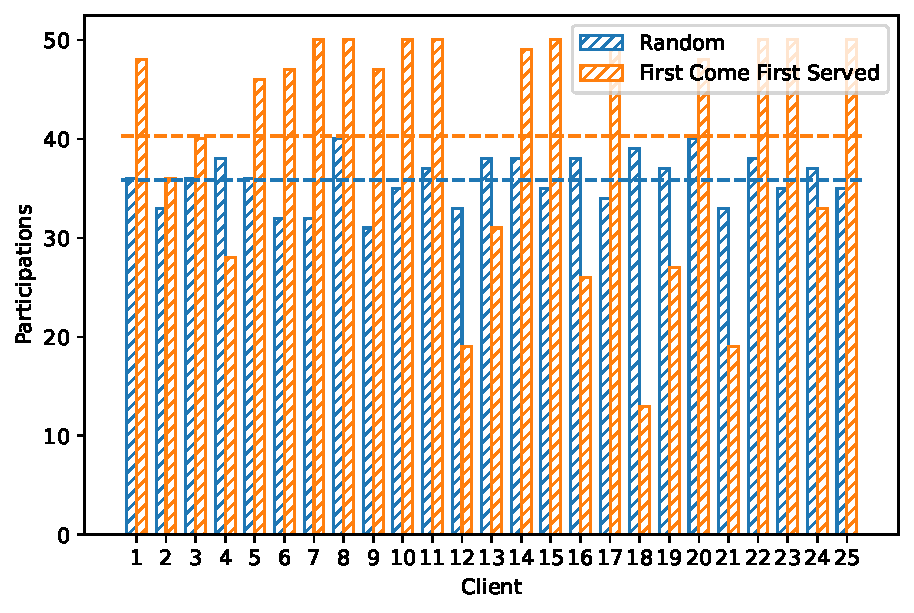
\includegraphics[width=0.7\textwidth]{graphics/selection/clients.pdf}
    \caption{Participation of Each Client Per Selection Algorithm}
    \label{fig:participations_client}
\end{figure}

On one hand, random selection presents a more uniform distribution, where each client was selected a similar number of times. On the other hand, first-come first-served presents a more skewed distribution, where some clients, such as client 1, participate many times and others, such as client 12, participate very few times. To support this observation, we calculated the standard deviation. For the random selection, the standard deviation is approximately 2.49, while for the first-come first-served it is 11.84.

From this observations, we can conclude that, by letting clients take initiative to join a round, like what happens in first-come first-served, it is possible that some will end up participating more than others. By participating more often, the clients will have more influence on the global model, which can lead to skewed results.

\subsection{Execution Time, Transaction Cost, and Transaction Latency}

Regarding execution time, it can be seen from  \autoref{tab:metrics_selection} that both algorithms only differ in approximately $1.2$ minutes, which translates to a difference of $1.1$ seconds per round. In addition, the random participation was slightly faster than the first-come first-served. This negligible difference is likely caused by the fact that, in random selection, less clients participated on average per round, as shown in \autoref{fig:participations_client}. With slightly less clients, we expect that a round takes slightly less time.

\begin{table}[!ht]
\begin{tabular}{c|c|c} \hline \hline
                              & First Come First Served & Random \\ \hline \hline
E2E Time (m)                   & 19.70                   & 18.93  \\ \hline
Mean Round Time (s)            & 23.62                   & 22.70  \\ \hline
% Median Round Time (s)          & 22.06                   & 21.90  \\ \hline
Mean Transaction Latency (s)   & 1.560                   & 1.549  \\ \hline
% Median Transaction Latency (s) & 1.561                   & 1.549  \\ \hline
Mean Transaction Cost (Gas)    & 189179                  & 183124 \\ \hline
% Median Transaction Cost (Gas)  & 223471                  & 185198 \\ \hline
\end{tabular}
\caption{Execution Time, Transaction Cost, and Transaction Latency Per Participant Selection Algorithm}
\label{tab:metrics_selection}
\end{table}

\subsection{Model Accuracy and Convergence}

As it can be seen from \autoref{fig:accuracy_selection}, even though both algorithms reached identical model accuracy values at the last round, the random selection was more stable during the initial 20 rounds. This can be explained by the fact that the distribution of clients participating in each round with the random selection was closer to a uniform selection. Since the data is \textit{non-iid}, by having the same clients participate repeatedly, the model can become skewed towards their data. However, after 20 rounds, the majority of the clients had the opportunity to participate in the model, which explains why it became more and more stable.

\begin{figure}[!ht]
    \centering
    \centering
    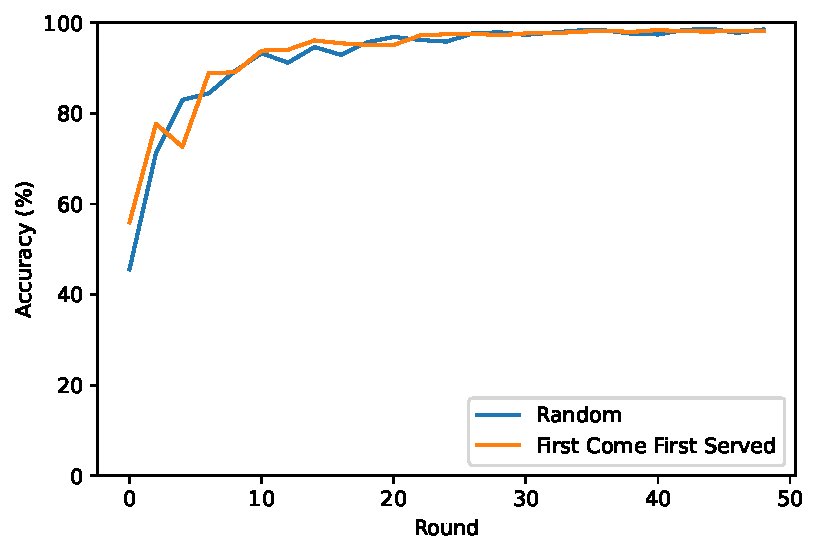
\includegraphics[width=0.7\textwidth]{graphics/selection/accuracy.pdf}
    \caption{Model Accuracy Per Participant Selection Algorithm}
    \label{fig:accuracy_selection}
\end{figure}

\subsection{Communication Costs}

\autoref{fig:net_selection} illustrates the network traffic per round for client, servers, and the blockchain processes. This algorithms solely influences which and how many clients are selected per round. Therefore, the individual communication traffic of each process is not expected to change significantly as long as the number of participants per round does not change significantly. In these experiments, we observe form \autoref{fig:participations_client} that the difference of clients participating per round is smaller than $5$. This small difference explains why the inbound traffic at the server process is slightly higher, since the server has to download weights from a higher number of clients in order to perform the aggregation.

\subsection{Computation Costs}

\autoref{fig:ram_selection} and \autoref{fig:cpu_selection} show the RAM usage and CPU usage per each process, respectively. Similarly to what was observed regarding the communication costs, the RAM usage at the server is slightly higher, which is explained by the additional weights to perform the aggregation. One may note that this difference happens due to the randomness of the process. In other runs, it is possible that the number of selected devices would be lower and therefore the difference would be smaller.

\subsection{Conclusions}

From this set of experiments, we conclude that random selection performs better in terms of fairness of selection, that is, every client is given an equal chance of participating during the training process. In systems with \textit{non-iid} data, it is important to give all clients a chance to participate such that the model is trained with the most diverse data in order to produce the best results. Use of the random selection can ensure that the most amount of data is seen from most clients.

\section{Scoring Algorithms}

In this set of experiments, all properties of the system are static, except for the scoring algorithm, which varies between BlockFlow, Marginal Gain, Multi-KRUM, or no scoring algorithm. Then, we analyze the impact of using different numbers of clients, as well as different privacy degrees.

\subsection{Overall Comparison}\label{horizontal:scoring_overall}

We first compare the impact of the different scoring algorithms on the overall system without varying the number of clients or the privacy degree. This will let us draw some initial conclusions about the different scoring algorithms that may help explain differences observed in the remaining experiments.

\subsubsection{Execution Time, Transaction Cost, and Transaction Latency}

As it can be seen from \autoref{tab:metrics_scoring}, every scoring algorithm has different execution time and transaction cost. Firstly, one may notice that not using a scoring algorithm provides the fastest execution time as well as the lowest transaction cost. Both of these observations are explained by the fact that scoring algorithms require more transactions to submit the scores. Overall, the fastest scoring algorithm is Multi-KRUM, taking around $31$ seconds per round, while both BlockFlow and Marginal Gain are the slowest, taking both around $49$ seconds per round.

\begin{table}[!ht]
\centering
\begin{tabular}{c|c|c|c|c} \hline \hline
                               & None   & BlockFlow & Marginal Gain & Multi-KRUM \\ \hline \hline
E2E Time (m)                   & 18.93  & 40.95     & 41.38         & 26.25      \\ \hline
Mean Round Time (s)            & 22.70  & 49.11     & 49.64         & 31.48      \\ \hline
% Median Round Time (s)          & 21.90  & 49.49     & 43.97         & 31.26      \\ \hline
Mean Transaction Latency (s)   & 1.549  & 1.564     & 1.577         & 1.573      \\ \hline
% Median Transaction Latency (s) & 1.549  & 1.558     & 1.564         & 1.551      \\ \hline
Mean Transaction Cost (Gas)    & 183124 & 339645    & 257686        & 280733     \\ \hline
% Median Transaction Cost (Gas)  & 185198 & 189092    & 188994        & 187152     \\ \hline
\end{tabular}
\caption{Execution Time, Transaction Cost, and Transaction Latency Per Scoring Algorithm}
\label{tab:metrics_scoring}
\end{table}

Secondly, we observe that BlockFlow and Marginal Gain not only take the longest, but also have similar execution times. As explained in \Cref{background:scoring}, BlockFlow and Marginal Gain scores are computed by the clients, whereas Multi-KRUM scores are computed by the servers. Since the number of clients is higher than the servers, which are fixed, there are more devices performing scoring computations with BlockFlow and Marginal Gain. With more devices submitting scores, there are more transactions being submitted to the blockchain, leading to higher execution times. Therefore, it is expected that algorithms that run on the clients, such as BlockFlow and Marginal Gain, take longer than algorithms that run on the servers, such as Multi-KRUM.

Thirdly, we observe that the transaction latency is not influenced by the scoring algorithms. As it can be seen form \Cref{chapter:analysis:consensus_algorithms}, the transaction latency is mostly affected by the blockchain consensus algorithms, which, in these experiments, is fixed. In contrary, the transaction costs vary per scoring algorithm. Scoring algorithms that have more devices involved, such as scoring algorihtms executed by the servers, namely BlockFlow and Marginal Gain, have higher transaction costs. Since transaction costs work on a "supply and demand" basis, it is expected that the more transactions are required, the higher the cost will be.

\subsubsection{Model Accuracy and Convergence}

\begin{figure}[!ht]
    \centering
    \centering
    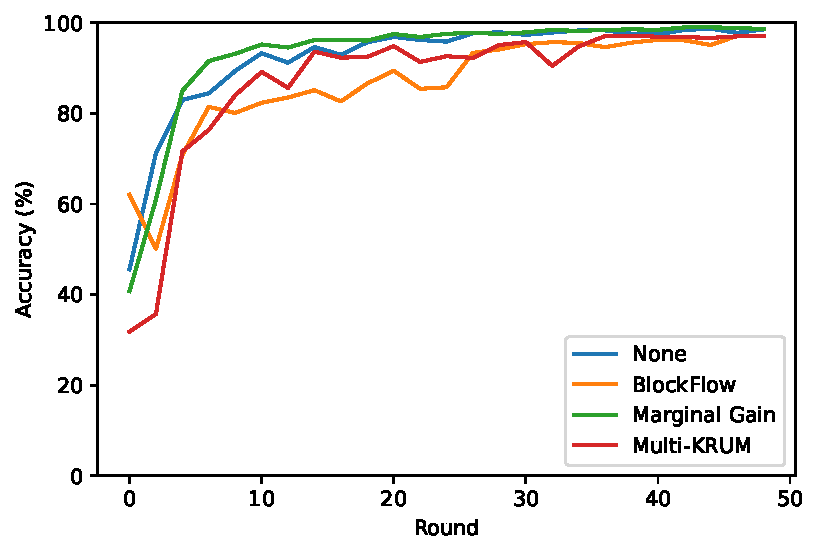
\includegraphics[width=0.7\textwidth]{graphics/scoring/accuracy.pdf}
    \caption{Model Accuracy Per Scoring Algorithm}
    \label{fig:accuracy_scoring}
\end{figure}

As it can be seen from \autoref{fig:accuracy_scoring}, all scoring algorithms reached a high model accuracy of at least  $97\%$. However, some algorithms reached higher accuracy values faster than others, that is, some converge faster. Overall, Marginal Gain converges the fastest, followed by no scoring, then by Multi-KRUM and lastly by BlockFlow.

The BlockFlow, is not only the slowest converging scoring algorithm, but also the only algorithm that does not reject submissions when aggregating, as explained in \Cref{background:scoring}. By not rejecting submissions, but still giving them a score to be used during the weighted aggregation, worse submissions are always included in the global model, which can lead to lower convergence rates. 

The Marginal Gain and Multi-KRUM algorithms both reject the worst submissions in each round and only consider the best. While the Marginal Gain uses its own score for the aggregation, the Multi-KRUM uses the number of samples of each submission, similar to the case when no scoring algorithm is used. For this reason, the Multi-KRUM algorithm convergence resembles the one of no scoring algorithm, while the Marginal Gain has a smoothest convergence curve.

\subsubsection{Communication Costs}

Communication costs also vary massively depending on which  scoring algorithm is used. Some place more strain on the clients, where others place more strain on the servers. \autoref{fig:net_scoring} presents the network traffic per round per scoring algorithm on the clients, servers, and blockchain processes.

Regarding the clients, there is a large difference in terms of the network traffic when comparing no scoring algorithm and the Multi-KRUM with the BlockFlow and Marginal Gain. On the one hand, the Multi-KRUM has similar traffic requirements to using no scoring algorithm on the clients because the scoring algorithm is executed on the servers. On the other hand, the BlockFlow and Marginal Gain have higher inbound traffic at the clients, while the outbound traffic remains similar. This can be explained by the fact that both BlockFlow and Marginal Gain algorithms are executed by the clients. Consequently, each client has to download the weights from all other clients in each round in order to calculate the score, leading to a higher inbound traffic.

Regarding the servers, there is not much difference between algorithms, except for the Multi-KRUM, which calculates the scores on the server. Therefore, the server downloads the weights of each client and requires additional time to calculate the scores, compared to the remaining algorithms that only download the weights once for the aggregation.

Finally, regarding the blockchain, we observe that when using the BlockFlow and Marginal Gain algorithms that there is a higher network traffic. The Multi-KRUM also requires more traffic than no scoring algorithm, but not as much as the BlockFlow or Marginal Gain. Since the number of clients is higher than the number of servers, there are more transactions when the scoring algorithm runs on the clients. When there are more transactions per round, there is more activity in the blockchain, leading to more network traffic per round.

\subsubsection{Computation Costs}

The computation costs across the servers and clients follow a similar trend to what we have seen with the communication costs. \autoref{fig:ram_scoring} and \autoref{fig:cpu_scoring} show the RAM and CPU usages on the client, server and blockchain processes, respectively.

Regarding the clients, all algorithms require similar amounts of RAM. The algorithms that run on the client, i.e., the Marginal Gain and BlockFlow, consume slightly more RAM, due to having more weights stored in memory, but the difference is negligible when compared to the total amount of RAM they consume. This can be explained by the fact that the weights are relatively small ($\approx 2$ MB) compared to the total RAM necessary to train a model. With respect to the CPU usage, it can be seen that the algorithms that run on the client, i.e., BlockFlow and Marginal Gain, have the lowest CPU idle time on the clients, while taking longer to be executed. This shows that calculating the scores on the client implies consistently higher CPU usage on the clients for longer periods of time.

Regarding the servers, it is clear that Multi-KRUM, being the only scoring algorithm that runs on the server, requires higher amount of RAM. However, the difference ($\approx 15$ MB) is not significant when considering that the servers have large amount of resources at their disposal. In addition, the Multi-KRUM also shows higher level of CPU usage, with frequent spikes to $100\%$.

Finally, regarding the blockchain, the difference of CPU and RAM usages among the different scoring algorithms is negligible. Even though the blockchain receives more transactions in total, it does not reflect on the RAM and CPU usage. The blockchain, by itself, already produces blocks at a constant rate. Therefore, the number of transactions required for the BFL system does not change significantly the CPU or RAM usage.

\subsubsection{Conclusions and Improvements}

In conclusion, scoring algorithms that are executed on the clients, i.e.,the Marginal Gain and BlockFlow, have a higher impact on the overall system, leading to longer experiment execution times and higher resource usage for the clients. In contrary, algorithms that are executed on the servers, i.e., the Multi-KRUM, have a higher impact on the servers. Since there is usually a much higher number of clients than servers, the scoring algorithms executed by the servers have less impact on the overall system than the former. Additionally, the Marginal Gain was the most well performing algorithm in terms of model accuracy and convergence speed, followed by the Multi-KRUM and the BlockFlow.

If we had to choose an algorithm, the choices come down to the priorities of the system. If we are working with a system with resource-constrained devices, such as IoT systems, it is important that the impact on the clients is low. Therefore, scoring algorithms that run on the server, such as the Multi-KRUM, are more valuable. If the opposite is true, or if the resource consumption at the client is not relevant, the Marginal Gain could be chosen as it provides the best accuracy of the three.

It is also important to mention that algorithms that require more network traffic per round may be slower on clients with low bandwidth, which is the case of many IoT networks. With lower bandwidths, less traffic can go through at any point in time. Therefore, in case of high network traffic required during a round, devices with low bandwidth can make the process slower.

As a future improvement, servers can cache the client's update weights. Specifically, in case of the Multi-KRUM algorithm, the servers can download each of the client's submission twice: one time for scoring, one time for aggregating. However, the weights downloaded both times are the same as they are part of the same round. Therefore, caching can work well in favor of reducing the network traffic at the server for scoring algorithms that are executed by servers.

\subsection{Number of Clients}\label{horizontal:number_of_clients}

In this section, we analyze the impact of different numbers of clients on the scoring algorithms. For this comparison, all properties of the system are static, except for the amount of clients, which varies between 5, 10, 25 and 50, per each scoring algorithm.

\subsubsection{Execution Time, Transaction Cost, and Transaction Latency}

\autoref{fig:clients_metrics} illustrates the execution times, as well as the transaction latency and costs. The execution times of all scoring algorithms increase with the number of clients. However, they do not increase the same way. The Multi-KRUM algorithm, as well as not using any scoring algorithm, have a smaller execution time increase with the number of clients, when compared to BlockFlow and Marginal Gain. This can be explained by the fact that, in BlockFlow and Marginal Gain, the scorers are the clients. Since, as previously discussed, there are more clients than servers, the smart contract has to wait for more scorers to submit their scores, than it would have to wait when using Multi-KRUM. Consequently, the execution time increase with the number of devices is higher with scoring algorithms executed by the clients.

\begin{figure}[!ht]
    \centering
    \begin{subfigure}[b]{0.49\textwidth}
        \centering
        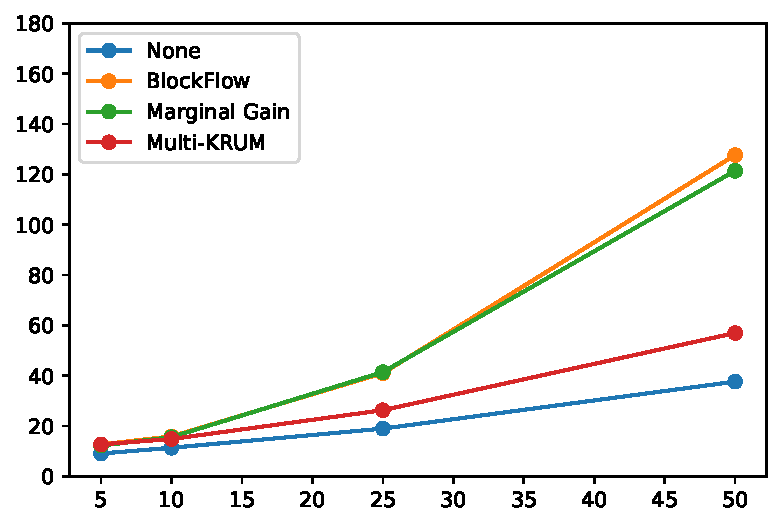
\includegraphics[width=\textwidth]{graphics/clients/e2e.pdf}
        \caption{E2E Time}
    \end{subfigure}
    \hfill
    \begin{subfigure}[b]{0.49\textwidth}
        \centering
        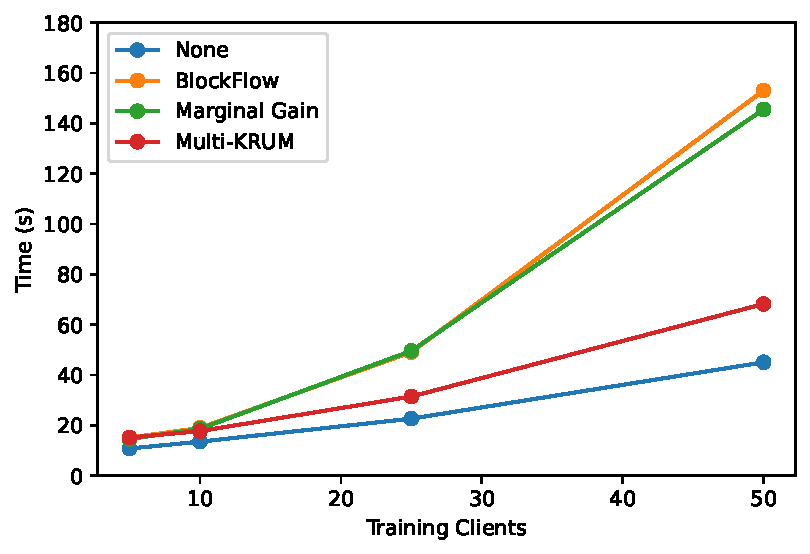
\includegraphics[width=\textwidth]{graphics/clients/round.pdf}
        \caption{Mean Round Time}
    \end{subfigure}
    \hfill
    \begin{subfigure}[b]{0.49\textwidth}
        \centering
        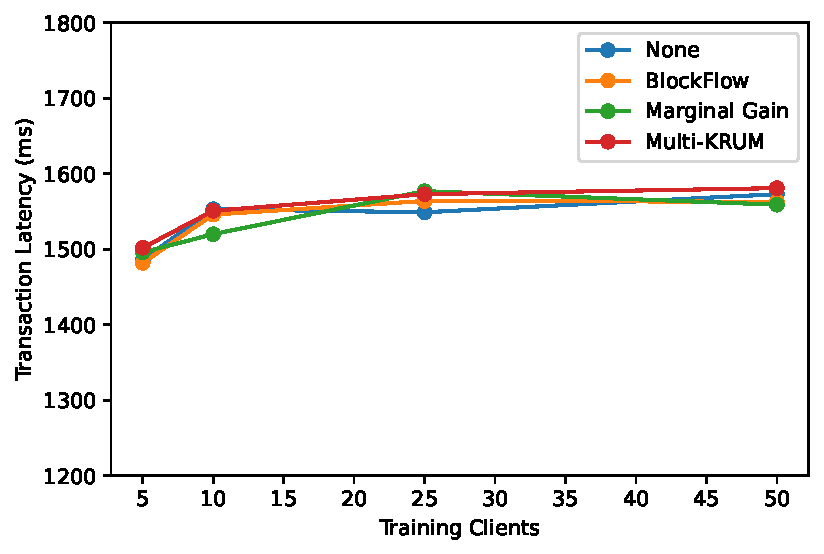
\includegraphics[width=\textwidth]{graphics/clients/tx_latency.pdf}
        \caption{Mean Transaction Latency}
    \end{subfigure}
    \hfill
    \begin{subfigure}[b]{0.49\textwidth}
        \centering
        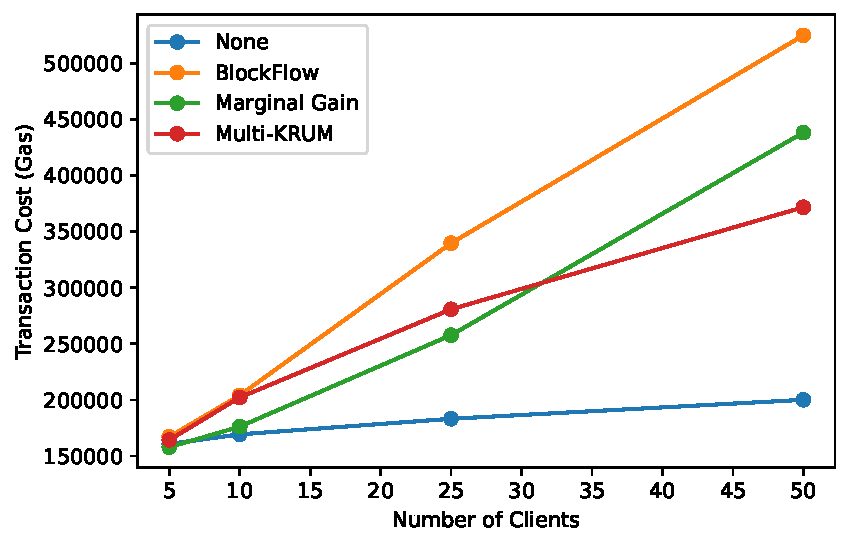
\includegraphics[width=\textwidth]{graphics/clients/tx_cost.pdf}
        \caption{Mean Transaction Cost}
    \end{subfigure}
    \caption{Execution Time, Transaction Cost, and Transaction Latency Per Number of Clients}
    \label{fig:clients_metrics}
\end{figure}

Regarding the transaction latency, there is no significant change with the variation of number of clients. As discussed before, transaction latency is mostly determined by the capacity of the network to handle the transactions. The Ethereum has a relatively fixed capacity of transactions per second of around 15 transactions per second. Our system alone does not reach that rate of transactions, not influencing the transaction latency. It is worth pointing out that, if the number of clients was in the order of hundreds, leading to elevated number of transactions, the latency would likely increase.

Regarding the transaction costs, we observe that they increase with the increased number of clients. In addition, the transaction costs growth is similar per algorithm. Firstly, we can calculate how many transactions we incur per algorithm per round by $T+A+S$, where $T$ is the number of trainers, usually clients, $A$ is the number of aggregators, usually servers, and $S$ the number of scorers, which can be either the clients or servers. When no scoring algorithm is used, the system only requires $T+A$ transactions, where $T$ is the number of clients and the only growing variable. With the Multi-KRUM, the system requires $T+2A$ transactions, since $S=A$, leading to a faster growth than when no scoring algorithm is used. Finally, both BlockFlow and Marginal Gain algorithms require $2T+A$ transactions and since $T > A$ and $T$ is the number of growing clients, it is also expected that the transaction cost would increase more than for the Multi-KRUM.

\subsubsection{Model Accuracy and Convergence}

As it can be seen from \autoref{fig:accuracy_clients}, the model accuracy and how it converges varies differently with different scoring algorithms. Overall, we observe that lower number of clients leads to a less stable convergence, represented by the spiking in the model accuracy plots. With a low number of clients, such as 5, the selected number of clients per round is also low due to the random way the participant selection algorithms chooses how many clients participate per round. Therefore, the model is trained with less diverse data per round. Consequently, the model can skew at some points during training, leading to a less stable convergence. In contrary, using more clients, namely 25 and 50, has an overall positive effect on both convergence stability and convergence speed. This is also likely related to the fact that the model is trained with more diverse samples from more clients in each round, leading to a better results.

\begin{figure}[!ht]
    \centering
    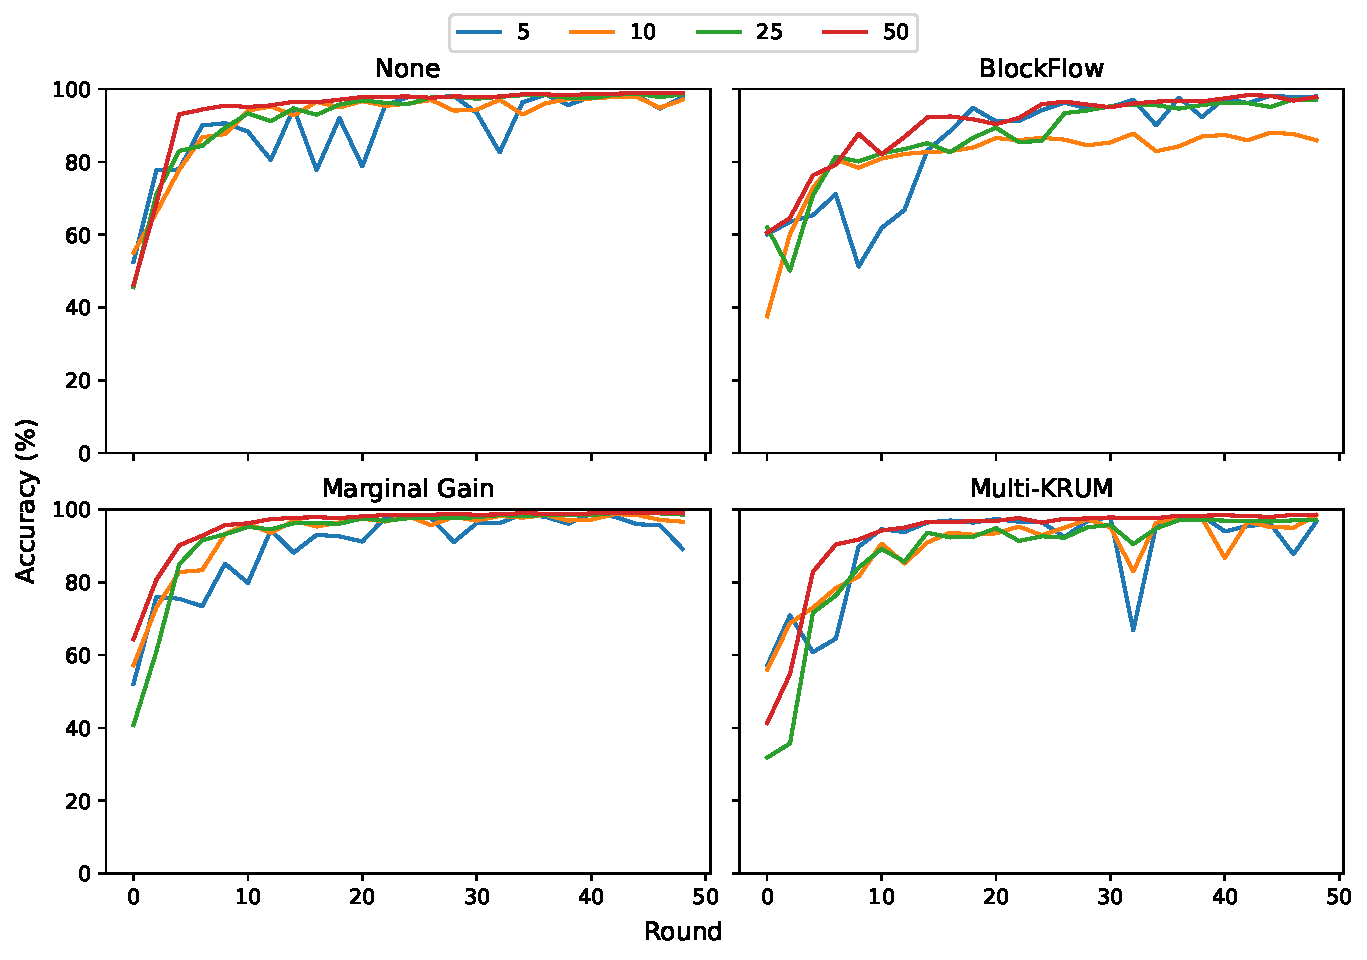
\includegraphics[width=\textwidth]{graphics/clients/accuracy.pdf}
    \caption{Model Accuracy Per Number of Clients}
    \label{fig:accuracy_clients}
\end{figure}

When it comes to the algorithm that performs best, the conclusions drawn from \Cref{horizontal:scoring_overall} remain true: the Marginal Gain performs the best, followed by the Multi-KRUM and finally by the BlockFlow.

\subsubsection{Communication Costs}

As it can be seen from \autoref{fig:net_clients}, the communication costs vary with the number of clients. Firstly, we observe that in terms of incoming traffic at the client process, there are significant differences depending on the scoring algorithm used.

\begin{figure}[!hb]
    \centering
    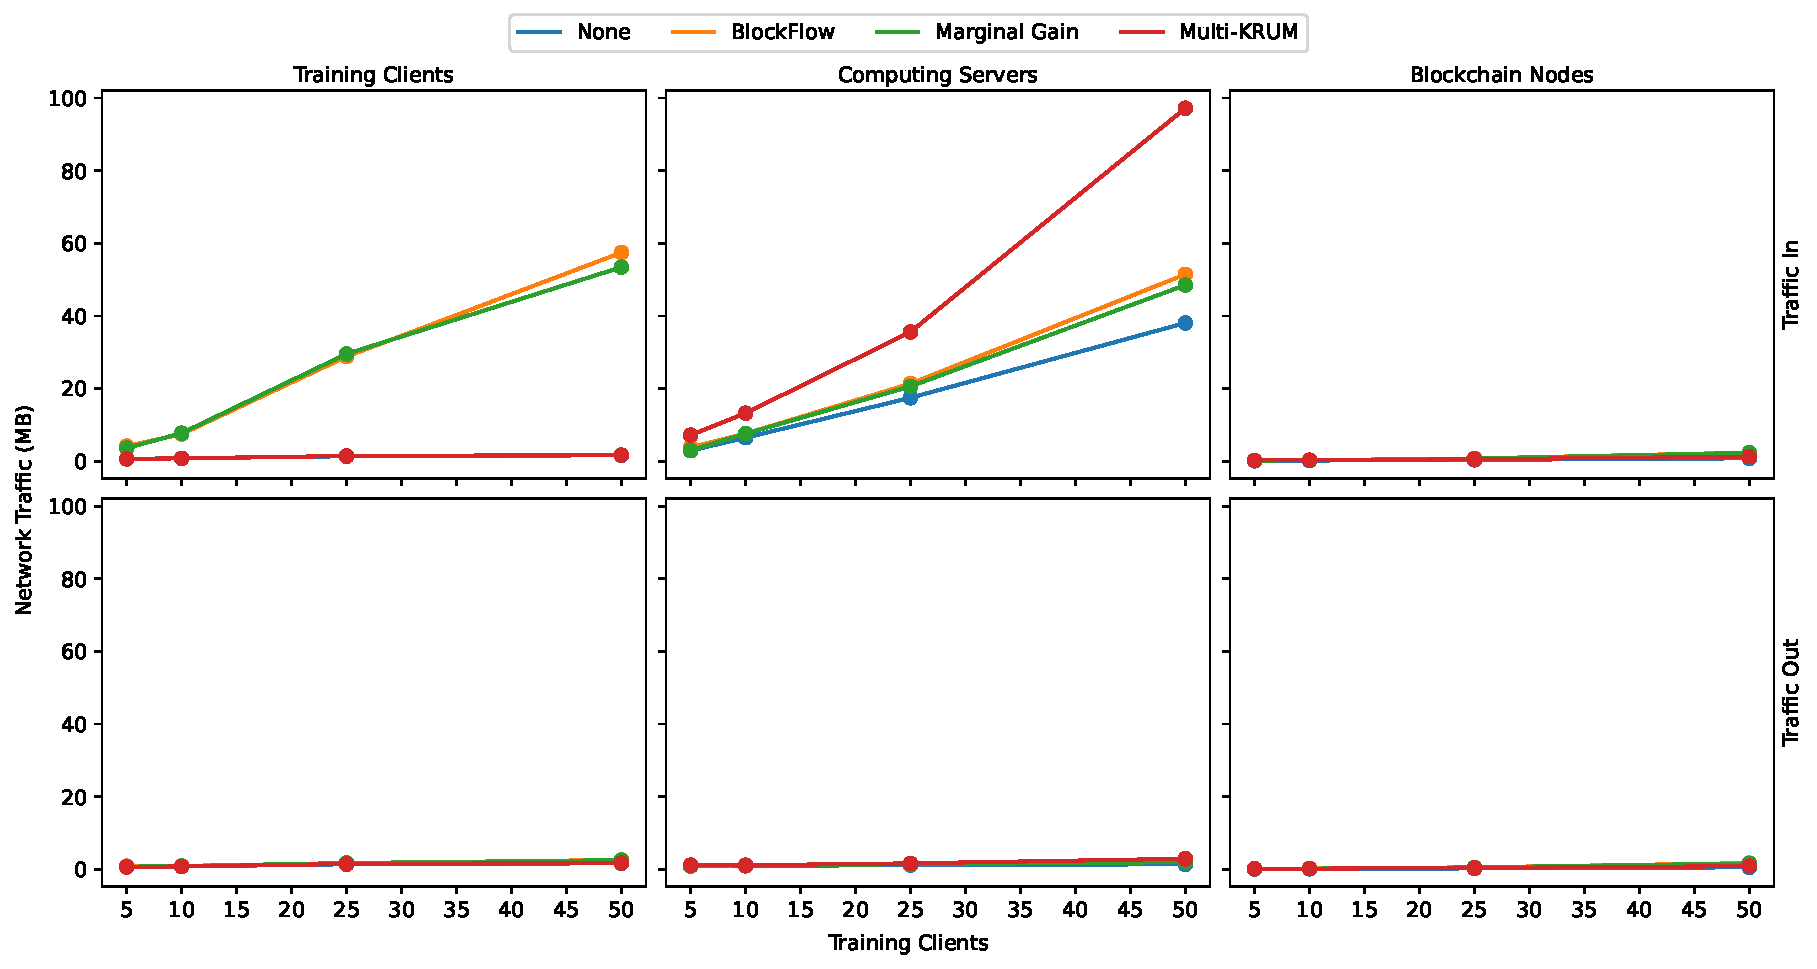
\includegraphics[width=\textwidth]{graphics/clients/traffic.pdf}
    \caption{Network Traffic Per Number of Clients}
    \label{fig:net_clients}
\end{figure}

One may notice that incoming traffic at the clients only increases when using scoring algorithms that are executed by the clients, such as the BlockFlow and the Marginal Gain. This can be explained by the fact that the more clients means the more weights from these clients need to be downloaded and scored. In contrary, when the scoring algorithm is executed by the server, there are virtually no changes in the incoming traffic when number of clients is increased. This is because the client only has to download the global weights after each round, which is not influenced by the number of clients.

Secondly, we observe that the incoming traffic always grows linearly at the servers when using a scoring algorithm that runs at the clients. However, when using a algorithm that runs on the server, such as the Multi-KRUM, the growth is higher than for the remaining algorithms. In all cases, the servers always have to download the weights for aggregation. However, if the scoring is executed at the servers, they will download the weights twice as explained in \Cref{horizontal:scoring_overall}, leading to a super-linear traffic growth. As previously suggested, this can be improved by caching the weights between these two phases.

Thirdly, we observe that the outgoing traffic differences are not significant for any of the processes. Regarding the clients and servers, we observe a very small increase on the client or server processes, if the scoring algorithm is executed by the clients or servers, respectively. However, the differences of outgoing traffic per number of clients for each scoring algorithm are negligible.

Finally, the differences observed in the blockchain process, both for incoming and outgoing traffic are negligible. With the increase of the number of clients, there are more transactions going through the blockchain. However, the transactions on the blockchain are very small when compared to the size of weights that need to be uploaded and downloaded by the clients and servers, respectively.

\subsubsection{Computation Costs}

\autoref{fig:ram_clients_clients}, \autoref{fig:ram_clients_servers}, \autoref{fig:ram_clients_miners} show the RAM usage at the clients, servers, and blockchain processes, while  \autoref{fig:cpu_clients_clients}, \autoref{fig:cpu_clients_servers}, \autoref{fig:cpu_clients_miners} show the CPU usage at the clients, servers, and blockchain processes, respectively. Overall, it can be seen that the number of clients has no major impact on RAM and CPU usage of either clients or servers.

Even though the usage of RAM and CPU at a certain points in time does not vary significantly, some scoring algorithms have more impact on the clients, or on the servers, as discussed in \Cref{horizontal:scoring_overall}. In addition, we observe that the increase of resource usage is proportional to the number of clients, depending on whether the the scoring algorithm is executed by the clients or the servers.

The only major change is observed in the RAM and CPU usage of the blockchain process. The higher the number of clients, the higher the RAM and CPU usage. This is expected as more clients are connected to the blockchain, meaning that more devices continuously interact and send transactions to the blockchain.

\subsubsection{Conclusions and Improvements}

In conclusion, scoring algorithms executed by the clients, i.e., the BlockFlow and Marginal Gain, show higher execution time increases with respect to the number of clients. In addition, the resource usage at the clients increases linearly with the number of devices. In contrary, algorithms executed by the servers, i.e., the Multi-KRUM, do not have significant effects on the clients' resources usage. Therefore, in systems with resource-constrained clients, algorithms executed by the server may be the ideal solution.

Finally, the resource usage of the blockchain process, mainly in terms of RAM, increases with the number of clients. The blockchain resource usage is an important aspect to consider in BFS systems. There is a clear trade-off between the number of clients with the blockchain resource usage.

\subsection{Privacy Degrees}

In this section, we analyze the impact of different privacy degrees on each scoring algorithm. In this set of experiments, all properties of the system are fixed, except for the degree of privacy, which varies between 0, 1 and 5, per each scoring algorithm.

\subsubsection{Execution Time, Transaction Cost, and Transaction Latency}

As it can be seen from \autoref{fig:priv_metrics}, having a privacy mechanism increases the execution time of each round by approximately $16.6$ seconds. In addition, the privacy degree itself does not seem to influence the execution time significantly.

% Therefore, we can conclude that there is a trade-off between execution time and privacy.

Regarding the transaction latency and costs, there are no significant differences. The privacy mechanism is executed by the clients before they submit their model update, and does not change the number of transactions. Consequently, it has no impact on the blockchain process itself.

% From this 16.6 seconds, 10 seconds directly caused by the differential privacy mechanism. The remaining are caused by slight fluctuations on communication time, such as waiting for all clients to submit their updates after applying the differential privacy.

\begin{figure}[!hpt]
    \centering
    \begin{subfigure}[b]{0.47\textwidth}
        \centering
        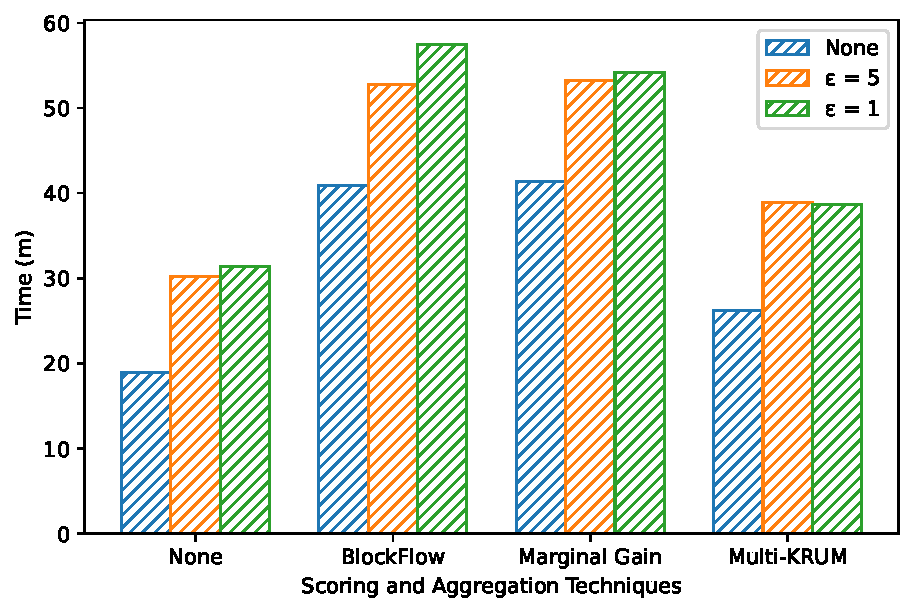
\includegraphics[width=\textwidth]{graphics/privacy/e2e.pdf}
        \caption{E2E Time}
    \end{subfigure}
    \hfill
    \begin{subfigure}[b]{0.47\textwidth}
        \centering
        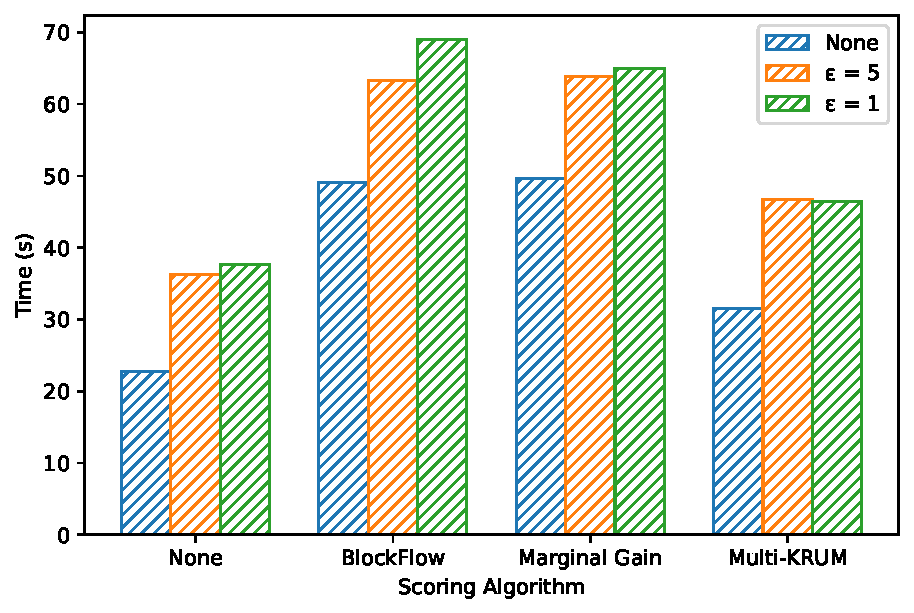
\includegraphics[width=\textwidth]{graphics/privacy/round.pdf}
        \caption{Mean Round Time}
    \end{subfigure}
    \hfill
    \begin{subfigure}[b]{0.47\textwidth}
        \centering
        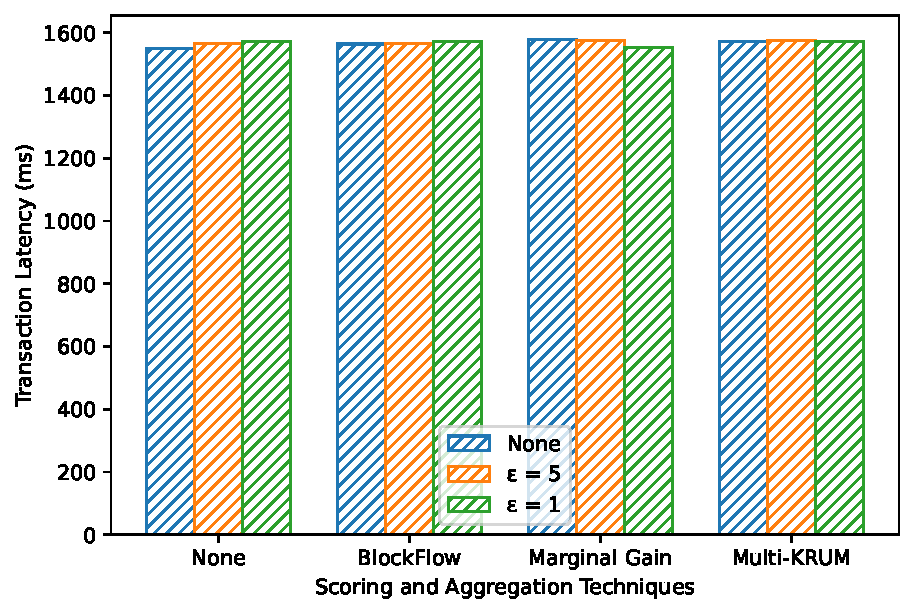
\includegraphics[width=\textwidth]{graphics/privacy/tx_latency.pdf}
        \caption{Transaction Latency}
    \end{subfigure}
    \hfill
    \begin{subfigure}[b]{0.47\textwidth}
        \centering
        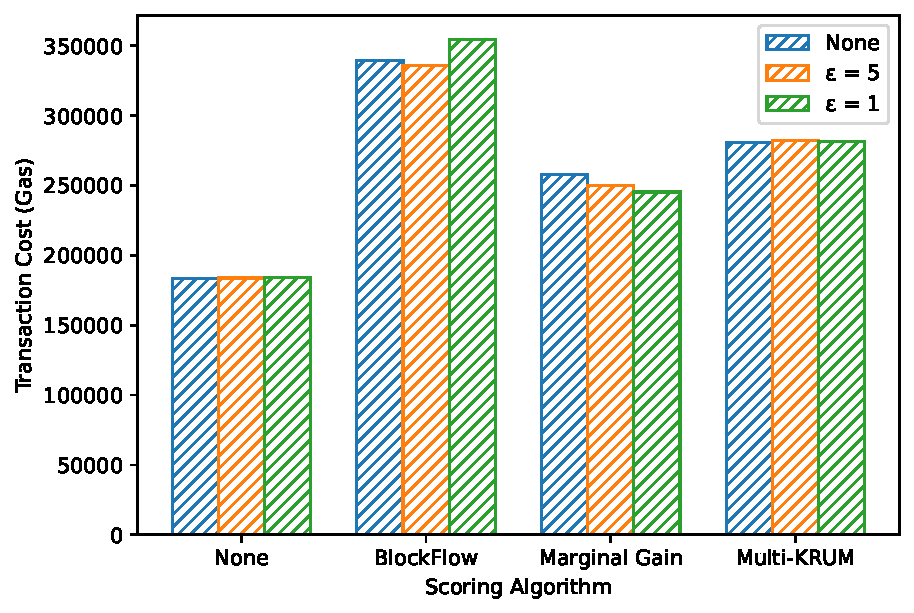
\includegraphics[width=\textwidth]{graphics/privacy/tx_cost.pdf}
        \caption{Transaction Cost}
    \end{subfigure}
    \caption{Execution Time, Transaction Cost, and Transaction Latency Per Privacy Degree}
    \label{fig:priv_metrics}
\end{figure}

\begin{figure}[!hpb]
    \centering
    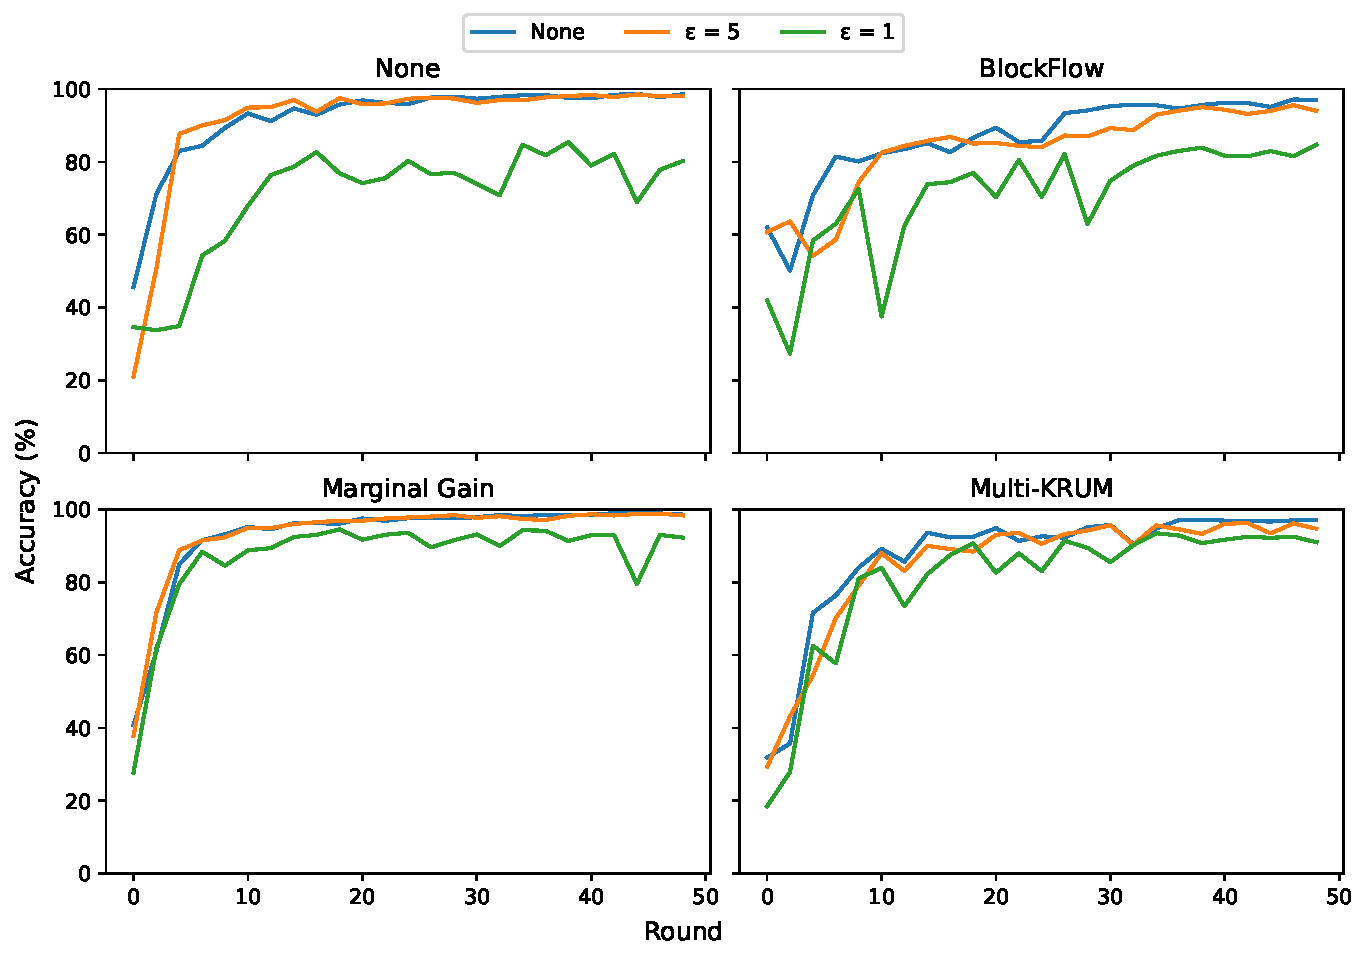
\includegraphics[width=\textwidth]{graphics/privacy/accuracy.pdf}
    \caption{Model Accuracy Per Privacy Degree}
    \label{fig:accuracy_privacy}
\end{figure}

\subsubsection{Model Accuracy and Convergence}

As it can be seen from \autoref{fig:accuracy_privacy}, different scoring algorithms have different accuracy drops using different privacy degrees. Overall, we observe that not using a scoring algorithm performs the worse with the highest degree of privacy, i.e., $\epsilon = 1$. In addition, a lower degree of privacy, i.e., $\epsilon = 5$, yields similar, yet lower, model accuracy than not using privacy degree. The higher the degree of privacy, the higher the noise values that are added to the original weights. Since the weights include added noise, it is expected that the accuracy will be lower with the higher degrees of privacy.

Out of the three scoring algorithms, the Marginal Gain and Multi-KRUM perform the best in presence of the higher degrees of privacy. As explained in \Cref{background:scoring}, both of these algorithms reject the worst updates, while BlockFlow does not. By rejecting the worst update, these algorithms always keep the best updates that provide the higher accuracy, even after noise is being added to the weights. Therefore, the Multi-KRUM and Marginal Gain have a lower accuracy drop with the higher privacy degrees, allowing them to maintain high model accuracy while preserving privacy.

\subsubsection{Communication Costs}

In terms of communication costs, as illustrated in \autoref{fig:net_privacy}, there are no significant differences depending on the privacy degree used. Adding noise to the weights does not necessarily increase their sizes and, for that reason, the network traffic costs are not expected to change significantly.

\subsubsection{Computation Costs}

\autoref{fig:ram_privacy_clients}, \autoref{fig:ram_privacy_servers}, \autoref{fig:ram_privacy_miners} show the RAM usage at the clients, servers, and blockchain processes, while \autoref{fig:cpu_privacy_clients}, \autoref{fig:cpu_privacy_servers}, \autoref{fig:cpu_privacy_miners} show the CPU usage at the clients, servers, and blockchain processes, respectively. Since the privacy algorithm is only executed by the client process, we only expect the computation costs, namely the CPU usage, to increase at the client process. Overall, we can observe that this is true as there are no significant changes in the RAM or CPU usage for the servers and blockchain processes.

As it can be seen from \autoref{fig:ram_privacy_clients}, the privacy mechanisms have no significant impact on RAM usage. The privacy algorithm has little RAM usage when compared to the total required for model training. In contrary, the CPU usage is higher, not necessarily in terms of usage percentage, but in terms of longer usage times. This can be seen from \autoref{fig:cpu_privacy_clients} and is explained by the time required for the execution of the privacy algorithm at the clients.

\subsubsection{Conclusions}

In conclusion, we see that using a privacy algorithm increases the computation costs, and consequently, the resource usage, at the clients. This leads to longer execution times as clients that need to process their weights and add noise to them. Therefore, there is a clear trade-off between execution time and privacy. However, increasing the privacy degree does not increase the execution time.

In addition, one may notice that increasing the privacy degree leads to the lower model accuracy. This is expected since the privacy algorithm used introduce noise to the weights. However, some of the scoring algorithms are still able to achieve higher model accuracy values even with higher privacy degrees. This is the case for the Marginal Gain and Multi-KRUM, which are the most well-performing algorithms.

Finally, we can argue that adding a privacy preserving algorithm to a BFS system is crucial, specially if the model is trained with sensitive data. One of the main arguments to apply blockchain to a Federated Learning system is the traceability and auditability. To do so, the weights, or their representation in our case, are recorded in the blockchain, which means they are visible and retrievable by anyone in the network. This implies that there is a trade-off between traceability and auditability and the requirement for privacy mechanisms, which in turn leads to higher resource usage.


% \chapter{Impact Analysis of Participants Selection Algorithms}\label{chapter:analysis:participants}
% In this chapter, we analyze the second experiment group, that is, the impact of using different participant selection techniques in a Blockchain-based Federated Learning system. In this set of experiments, all properties of the system are static, except for the participant selection mechanism, which varies between random selection, or "first come, first served", where the clients take initiative to join.

\section{Client Participation}

In both techniques, there is a factor of randomness. In random selection, both the amount of clients, as well as the clients themselves, are chosen randomly. In "first come, first served", only the amount of clients $C$ is chosen randomly. Then, after $C$ clients submit their updates, the round moves onto the next phase. This difference leads to the question: is the distribution of client participation going to be different? If so, how does it impact the model?

\begin{figure}[!ht]
    \centering
    \centering
    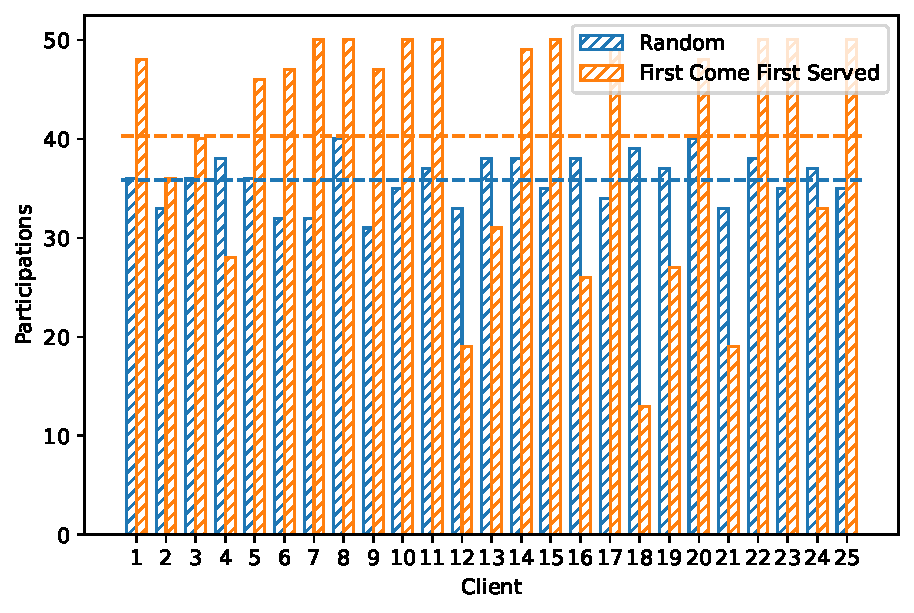
\includegraphics[width=0.7\textwidth]{graphics/selection/clients.pdf}
    \caption{Participation of Each Client Per Selection Technique}
    \label{fig:participations_client}
\end{figure}

To answer the questions, we first need to collect how many times each client participated in a round. On \autoref{fig:participations_client}, we can visualize how many times each client participated, represented by the bars, as well as the average amount of participation per client, represented by the lines. It is clear from the plot that the distributions are different. While the random selection presents a more uniform distribution, where each client was selected a similar amount of times, the "first come first served" selection presents more opposites, where some clients participate a high amount of times and others few times. The values of the standard deviation support this conclusion: for random selection, the standard deviation is approximately 2.49, while for "first come first served" it is 11.84.

This leads us to conclude that, by letting clients taking initiative to join a round, it is possible that some will end up participating more than others. In a system with heterogeneous devices, where some have more computation power than others, this may reveal to be an issue. Since more powerful devices are able to finish the training process faster, they are able to join the round earlier, allowing them to participate more times. By participating more times, they will have more influence over the global model in the end. This is not always desired as it may lead to skewed results.

\section{Execution Time, Transaction Cost and Latency}

Regarding execution time, we can see on \autoref{tab:metrics_selection} that both techniques only differ in around $1.2$ minutes, which translates to a difference of around $1.1$ seconds per round. We can see that random participation is faster than "first come first served". This small difference is likely caused by the fact that, in random selection, less participants participated on average per round, as seen in the previous section. With slightly less participants, it is expected for a round to take slightly less time.

\begin{table}[!ht]
\begin{tabular}{c|c|c} \hline \hline
                              & First Come First Served & Random \\ \hline \hline
E2E Time (m)                   & 19.70                   & 18.93  \\ \hline
Mean Round Time (s)            & 23.62                   & 22.70  \\ \hline
% Median Round Time (s)          & 22.06                   & 21.90  \\ \hline
Mean Transaction Latency (s)   & 1.560                   & 1.549  \\ \hline
% Median Transaction Latency (s) & 1.561                   & 1.549  \\ \hline
Mean Transaction Cost (Gas)    & 189179                  & 183124 \\ \hline
% Median Transaction Cost (Gas)  & 223471                  & 185198 \\ \hline
\end{tabular}
\caption{Time and Transaction Metrics Per Participant Selection Technique}
\label{tab:metrics_selection}
\end{table}

\section{Accuracy and Convergence}

When it comes to accuracy and convergence, we can see the data presented on \autoref{fig:accuracy_selection}. Even though both techniques reached virtually identical accuracy values in the end, random selection was more stable during the initial 20 rounds. This can be explained by the fact that the distribution of devices participating in each round with random selection was more uniform. Since the data is \textit{non-iid}, by having the same clients participate over and over, the model can become skewed. However, after 20 rounds, the majority of the devices had the opportunity to participate in the model, which explains why it became more and more stable.

\begin{figure}[!ht]
    \centering
    \centering
    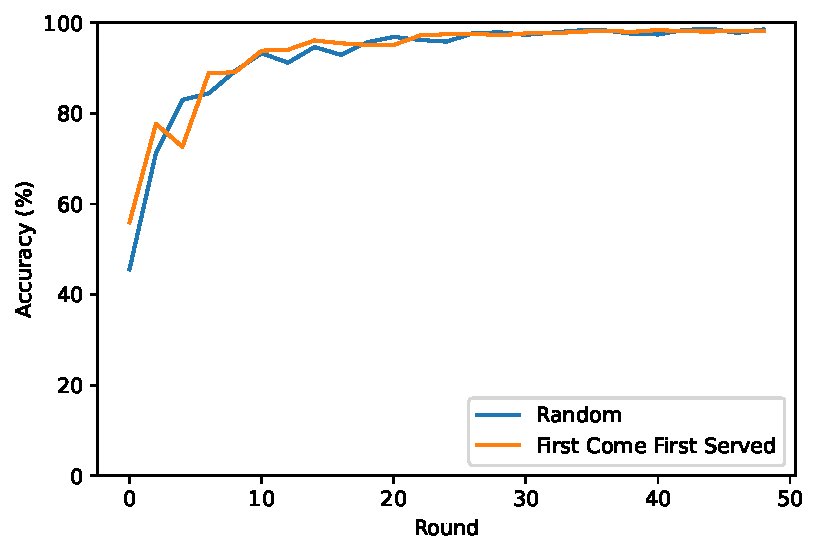
\includegraphics[width=0.7\textwidth]{graphics/selection/accuracy.pdf}
    \caption{Accuracy Per Participant Selection Technique}
    \label{fig:accuracy_selection}
\end{figure}

\section{Communication and Computation Costs}

Regarding communication and computation costs, it is expected that both techniques have similar results. On \autoref{fig:net_selection}, \autoref{fig:ram_selection} and \autoref{fig:cpu_selection}, we can visualize the network traffic per round, RAM usage and CPU usage, respectively, per each of the different devices. This techniques solely influences which and how many participants are selected per round. Therefore, the individual communication traffic is not expected to change significantly as long as the number of participants per round does not change significantly, which can be seen in the figures. In \Cref{chapter:analysis:participants}, we analyze in detail how much different amounts of participants actually impact communication and computation costs.

\begin{figure}[!ht]
    \centering
    \centering
    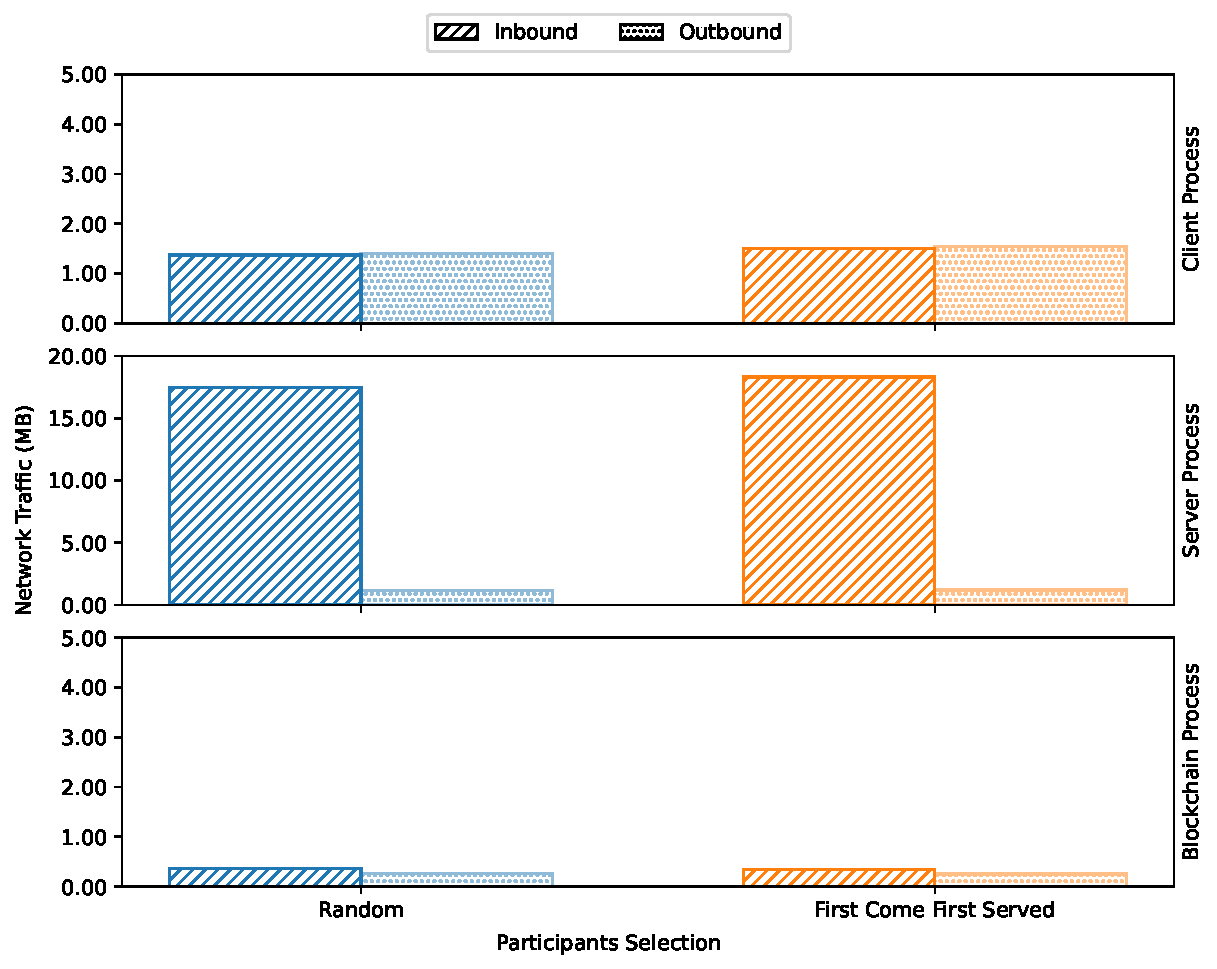
\includegraphics[width=0.8\textwidth]{graphics/selection/net.pdf}
    \caption{Network Traffic Per Round Per Participant Selection Technique}
    \label{fig:net_selection}
\end{figure}

\begin{figure}[!hpt]
    \centering
    \centering
    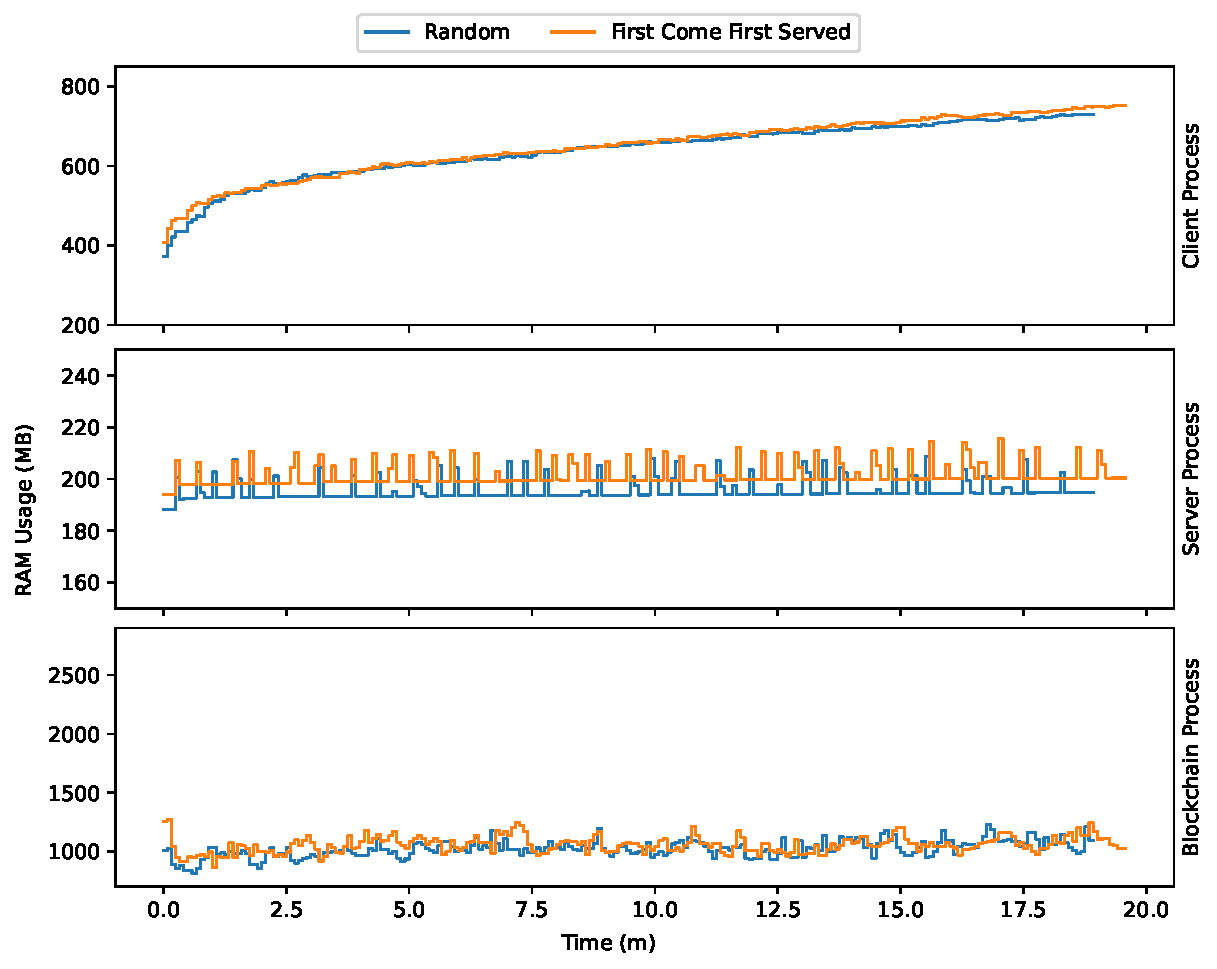
\includegraphics[width=0.8\textwidth]{graphics/selection/ram.pdf}
    \caption{RAM Usage Per Participant Selection Technique}
    \label{fig:ram_selection}
\end{figure}

\begin{figure}[!hpb]
    \centering
    \centering
    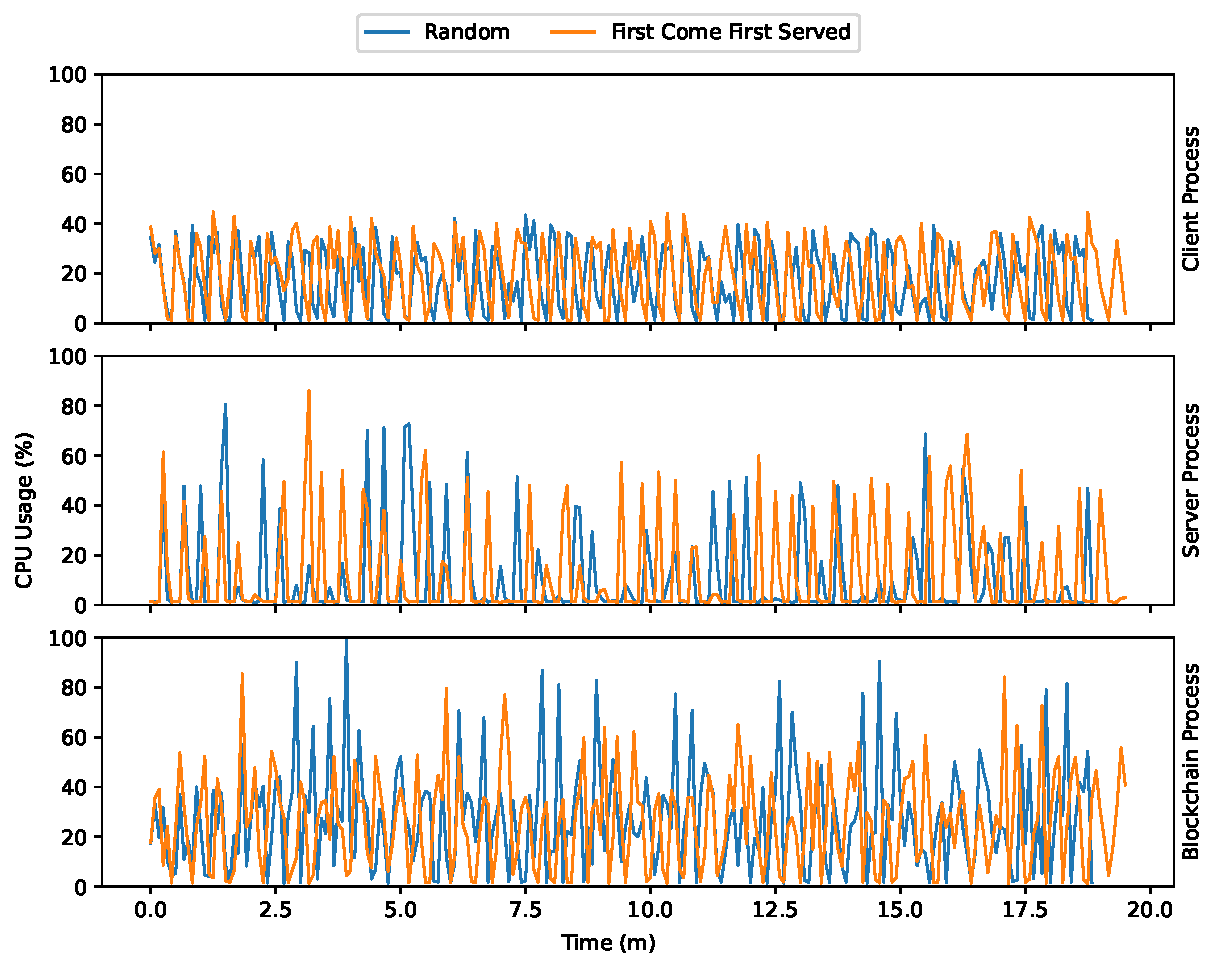
\includegraphics[width=0.8\textwidth]{graphics/selection/cpu.pdf}
    \caption{CPU Usage Per Participant Selection Technique}
    \label{fig:cpu_selection}
\end{figure}

\section{Conclusions and Improvements}

From this analysis, we can conclude that random selection performs better in the sense that it allows for a fairer selection of clients. In systems with \textit{non-iid} data, it is important to see the largest amounts of data in order to train the best model. By providing a uniform selection, all devices, and therefore their data, have equal changes of participating.

Finally, the "first come, first served" technique can also create a vector for vulnerability where more computationally powerful machines may be able to join more rounds if they end the training process earlier, exacerbating the aforementioned issue. With that being said, a possible future improvement is to change the moment in which a devices registers for a "first come, first served" round: instead of joining after training, it would join before the round. This would minimize the problem of computationally powerful devices repeatedly joining the rounds. % This could, however, lead to another potential problem when devices in constrained networks would not be able to participate as the round would close the registrations before they were able to join it.


% \chapter{Impact Analysis of Scoring Algorithms}\label{chapter:analysis:scoring}
% In this chapter, we analyze the third experiment group, that is, the impact of using different scoring algorithms in a Blockchain-based Federated Learning system. In this set of experiments, all properties of the system are static, except for the scoring algorithm, which varies between BlockFlow, Marginal Gain, Multi-KRUM, or none.

\section{Execution Time, Transaction Cost and Latency}

With respect to execution times, we can see on \autoref{tab:metrics_scoring} that every scoring algorithm gives different results. Since using no scoring algorithm means that there are less transactions and less computations, it is expected it will be the fastest. That is observable on \autoref{tab:metrics_scoring}, where it is shown that using no scoring algorithm is twice as fast as most scoring algorithms. The fastest scoring algorithm is Multi-KRUM, taking around $31$ seconds per round; while both BlockFlow and Marginal Gain are the slowest, taking both around $49$ seconds per round.

\begin{table}[!ht]
\centering
\begin{tabular}{c|c|c|c|c} \hline \hline
                               & None   & BlockFlow & Marginal Gain & Multi-KRUM \\ \hline \hline
E2E Time (m)                   & 18.93  & 40.95     & 41.38         & 26.25      \\ \hline
Mean Round Time (s)            & 22.70  & 49.11     & 49.64         & 31.48      \\ \hline
% Median Round Time (s)          & 21.90  & 49.49     & 43.97         & 31.26      \\ \hline
Mean Transaction Latency (s)   & 1.549  & 1.564     & 1.577         & 1.573      \\ \hline
% Median Transaction Latency (s) & 1.549  & 1.558     & 1.564         & 1.551      \\ \hline
Mean Transaction Cost (Gas)    & 183124 & 339645    & 257686        & 280733     \\ \hline
% Median Transaction Cost (Gas)  & 185198 & 189092    & 188994        & 187152     \\ \hline
\end{tabular}
\caption{Time and Transaction Metrics Per Scoring Algorithm}
\label{tab:metrics_scoring}
\end{table}

We can notice that BlockFlow and Marginal Gain, not only take the longest, but also take a very similar amount of time. As explained in \autoref{background:scoring}, BlockFlow and Marginal Gain scores are computed by other clients, where the Multi-KRUM is computed by the servers. Since the amount of clients is larger than the amount of servers, there are more devices performing scoring computations. For each scoring submission, there is a transaction. The more transactions there are, the more the system has to wait for the blockchain. In addition, clients are usually devices with less computational power. Therefore, it is expected that techniques that run on the clients, such as BlockFlow and Marginal Gain, take longer than techniques that run on the servers, such as Multi-KRUM.

On one hand, we can observe that transaction latency is not influenced by the scoring algorithms. The transaction latency, as seen before, is mostly influenced by the consensus algorithm, which, in this case, is static across the experiments. On the other hand, transaction costs are much higher when using a scoring algorithm. Scoring algorithms add at least one more transaction per round per device. Since transaction costs work on a "supply and demand" basis, it is expected that the more transactions are required, the higher the cost will be.

\section{Accuracy and Convergence}

\begin{figure}[!ht]
    \centering
    \centering
    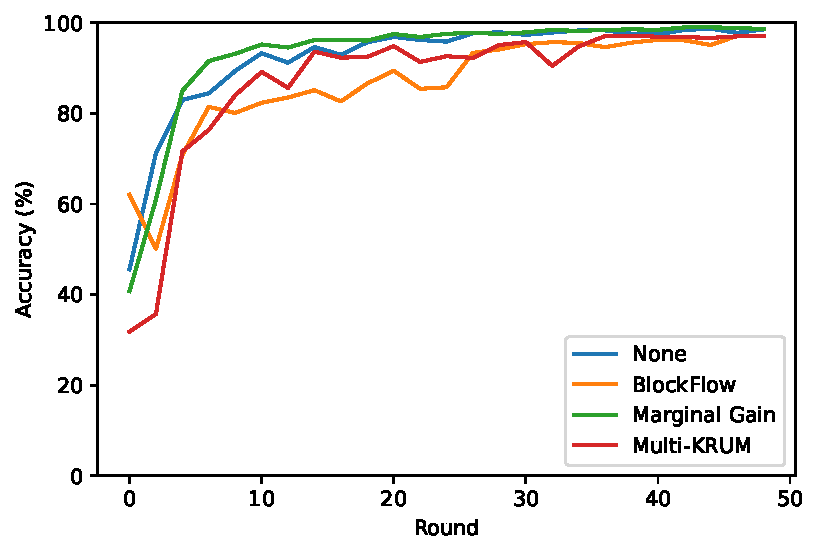
\includegraphics[width=0.7\textwidth]{graphics/scoring/accuracy.pdf}
    \caption{Accuracy Per Scoring Algorithm}
    \label{fig:accuracy_scoring}
\end{figure}

When comparing the accuracy across the different scoring algorithms, we can see on \autoref{fig:accuracy_scoring} that all techniques reached a high accuracy of above $97\%$. However, some techniques reach higher values faster than others, that is, some converge faster than others. As we can see, Marginal Gain converges the fastest, followed by no scoring, then Multi-KRUM and lastly BlockFlow.

On one hand, BlockFlow, is not only the slowest converging scoring algorithm, but also the only technique that does not drop submissions when aggregating. By not dropping submissions, but still giving them a score that is used during the weighted aggregations, worse submissions are always considered for the global model, which can lead to lower convergence rates. 

On the other hand, Marginal Gain and Multi-KRUM both drop the worst submissions in each round, only considering the best. While Marginal Gain uses its own score for the aggregation, Multi-KRUM uses the amount of samples of each submission, similarly to not using a scoring algorithm. For that reason, Multi-KRUM convergence resembles the one of no scoring algorithm, while Marginal Gain has a smoothest convergence curve.

\section{Communication Costs}

Communication costs also vary massively depending on the scoring algorithm in use. Some place more strain on the training clients, where others place more strain on the computing servers. On \autoref{fig:net_scoring}, we can visualize the network traffic per round per scoring algorithm on the clients, servers and blockchain nodes.

\begin{figure}[!ht]
    \centering
    \centering
    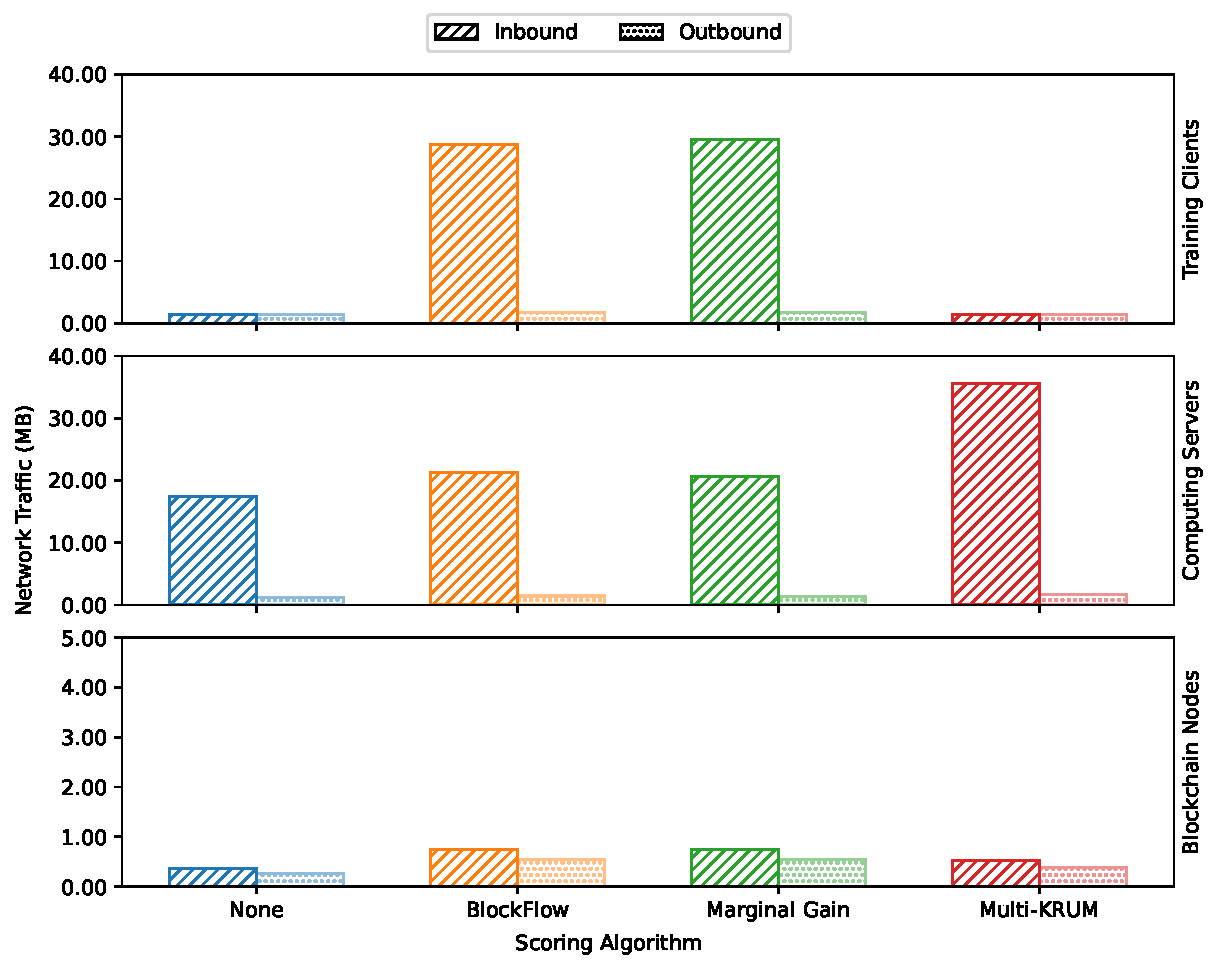
\includegraphics[width=0.8\textwidth]{graphics/scoring/net.pdf}
    \caption{Network Traffic Per Round Per Scoring Algorithm}
    \label{fig:net_scoring}
\end{figure}

Regarding the training clients, there is a large difference on the network traffic when comparing no technique and Multi-KRUM with BlockFlow and Marginal Gain. On the one hand, Multi-KRUM has similar traffic requirements to using no technique on the clients because the scoring algorithm is executed on the servers. On the other hand, BlockFlow and Marginal Gain require higher levels of inbound traffic, while the outbound traffic remains similar. This phenomenon can be explained by the fact that BlockFlow and Marginal Gain algorithms are executed on the training clients. Since the scoring algorithm is executed on the clients, each client has to download the weights from all the other clients in each round in order to calculate the score, leading to a much higher level of inbound traffic.

Regarding the computing servers, there is not much difference between techniques, except for the Multi-KRUM technique. Multi-KRUM calculates the scores on the server. Therefore, the server has to download the weights of each client's submission an additional time to calculate the scores, compared to the remaining techniques that only download the weights once for the aggregation.

Finally, regarding the blockchain nodes, we can visualize that when using the BlockFlow and Marginal Gain techniques that there is higher network traffic. Multi-KRUM also requires more traffic than no scoring algorithm, but not as much as BlockFlow or Marginal Gain. This can be explained by the same fact mentioned before: while BlockFlow and Marginal Gain run on clients, Multi-KRUM runs on servers. Since the number of clients is usually higher than the number of servers, there are more transactions when the scoring algorithm runs on the clients. When there are more transactions per round, there is more activity in the blockchain nodes, leading to more network traffic per round.

\section{Computation Costs}

The computation costs across the servers and clients follow a similar trend to what we have seen with the communication costs. On \autoref{fig:ram_scoring} and \autoref{fig:cpu_scoring}, you can visualize the RAM usage, and CPU usage, respectively, on the training clients, computing servers and blockchain nodes during the execution of the experiment.

Regarding the training clients, all techniques require similar amounts of RAM. The techniques that run on the client, Marginal Gain and BlockFlow, consume slightly more RAM, due to having more weights stored in memory, but the difference is negligible when compared to the total amount of RAM it consumes. This can be explained by the fact that the weights are relatively small ($\approx 2$ MB) compared to the total RAM necessary to train a model.

With respect to the CPU consumption, even though it looks similar, it is quite different. On previous analysis, such as in \Cref{chapter:analysis:consensus_algorithms}, we have seen certain techniques end earlier and therefore no data after a certain point. While on those analysis the slower techniques would have high amounts of idle CPU time on the clients, it is not the case here. The techniques that take the longest, that is BlockFlow and Marginal Gain, also have lowest amounts of CPU idle time. This confirms that calculating the scores on the client implies consistently higher CPU usage on the clients.

Regarding the computing servers, it is clear that Multi-KRUM, being the only scoring algorithm that runs on the server, requires higher amounts of RAM. However, the difference ($\approx 15$ MB) is not significant when considering that the computing servers have large amounts of resources at their disposal. In addition, Multi-KRUM also shows higher levels of CPU consumption, with frequent spikes to $100\%$.

Finally, regarding the blockchain nodes, the difference of CPU and RAM consumption is negligible as expected. Even though the blockchain receives more transactions in total, that does not reflect on the RAM and CPU consumption. The blockchain, by itself, already produces blocks at a constant rhythm. Therefore, the amount of transactions required for the BFL system does not change significantly the consumption.

\begin{figure}[!hpt]
    \centering
    \centering
    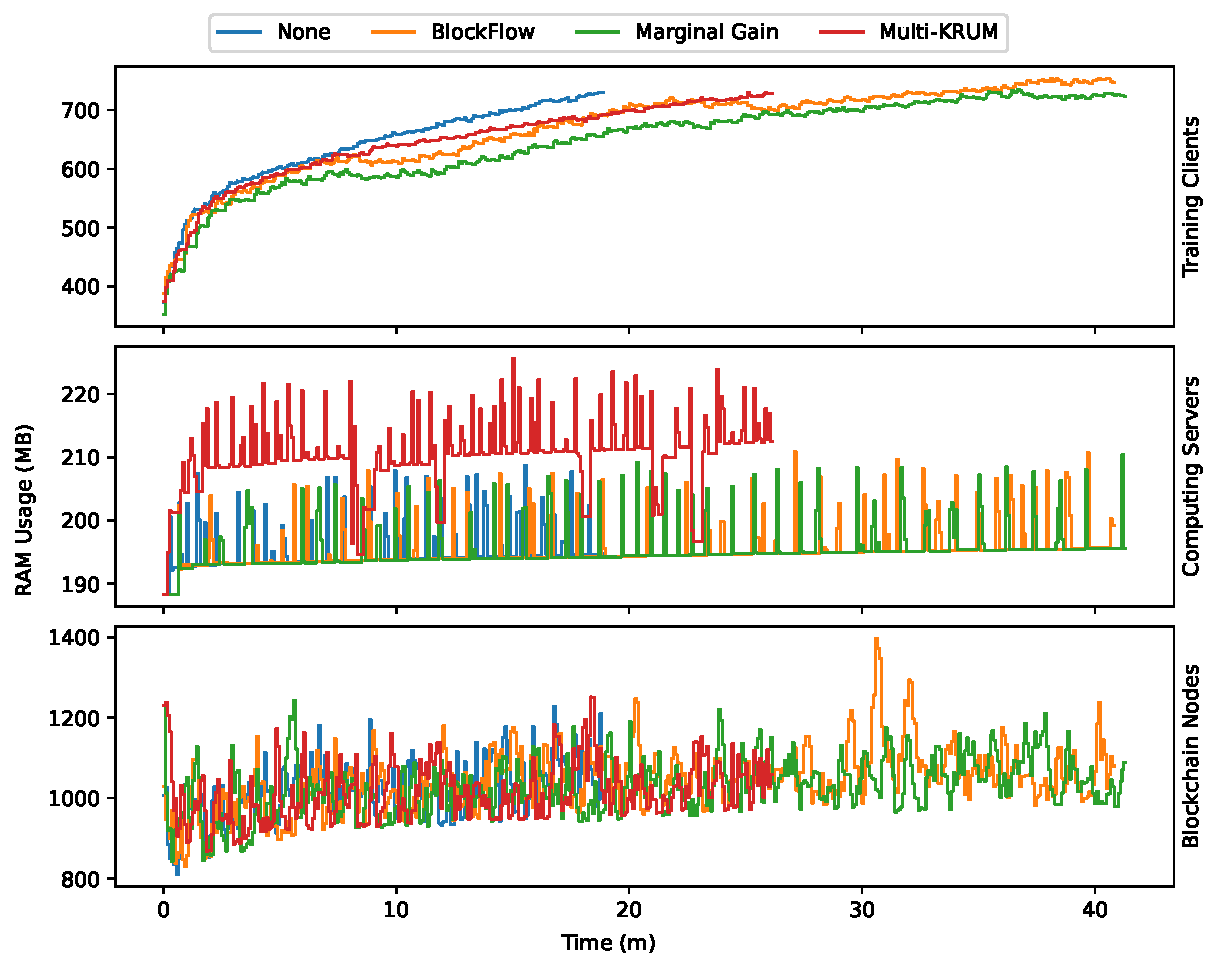
\includegraphics[width=0.8\textwidth]{graphics/scoring/ram.pdf}
    \caption{RAM Usage Per Scoring Algorithm}
    \label{fig:ram_scoring}
\end{figure}

\begin{figure}[!hpb]
    \centering
    \centering
    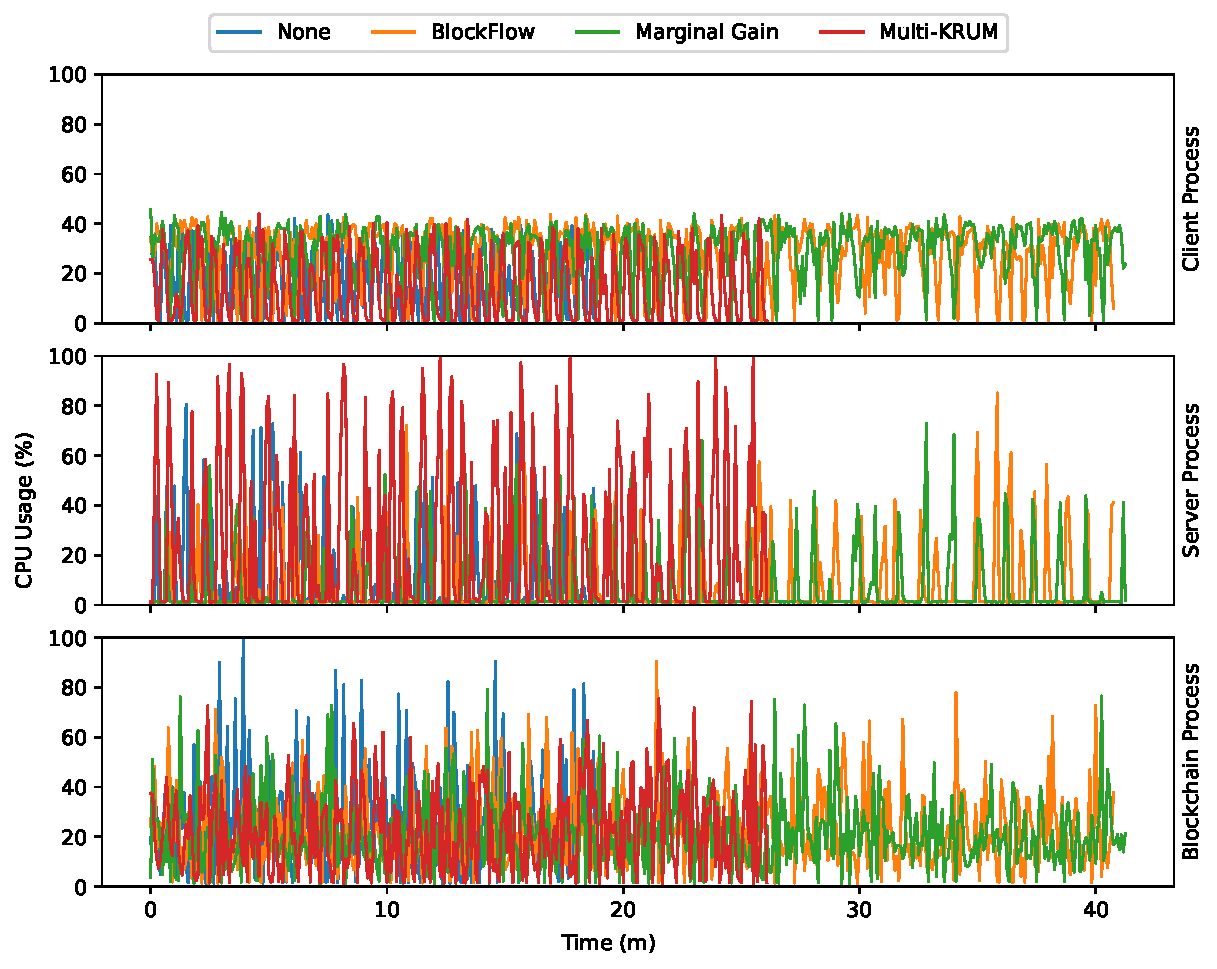
\includegraphics[width=0.8\textwidth]{graphics/scoring/cpu.pdf}
    \caption{CPU Usage Per Scoring Algorithm}
    \label{fig:cpu_scoring}
\end{figure}

\vfill

\section{Conclusions and Improvements}

In conclusion, scoring algorithms that are executed on the clients have a higher impact on the overall system in general, leading to higher round times and higher resource consumption for the clients. In contrast, techniques that are executed on the servers have a higher impact on the servers. Since there is usually a much higher amount of servers than clients, the latter have less impact on the overall system than the former. Additionally, Marginal Gain was the most well performing technique in terms of accuracy and convergence speed, followed by Multi-KRUM and BlockFlow.

If we had to choose between techniques, the choices come down to the priorities of the system. If we are working with a system with low-powered devices, such as IoT systems, it is important that the impact on the clients is lower. Therefore, scoring algorithms that run on the server, such as Multi-KRUM, are more valuable. If the opposite is true, or if the resource consumption at the client is not relevant, Marginal Gain could be chosen as it provides the best accuracy of the three.

It is also important to mention that techniques that require more network traffic per round might be slower when using clients with low bandwidth, which is the case of many IoT networks. With lower bandwidths, less traffic can come through at a point in time. Therefore, if there is a high amount of traffic required to be transmitted during a round, devices with low bandwidth can make the process slower.

As a future improvement, servers could cache the information about the weights of the submissions. Specifically, in the Multi-KRUM technique, the servers download each of the client's submission twice: one time for scoring, one time for aggregating. However, the weights downloaded in both of this times are the exact same since they are part of the same round and tied to the same submission. Therefore, caching can work well in favor of reducing the network traffic at the server for this type of techniques.


% \chapter{Impact Analysis of Number of Clients}\label{chapter:analysis:clients}
% \section{Execution Time, Transaction Cost and Latency}

\begin{figure}[!ht]
    \centering
    \begin{subfigure}[b]{0.49\textwidth}
        \centering
        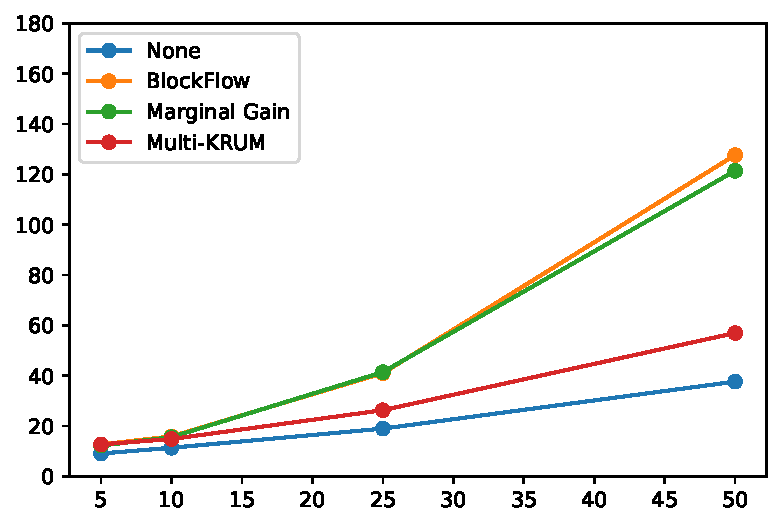
\includegraphics[width=\textwidth]{graphics/clients/e2e.pdf}
        \caption{E2E Time}
    \end{subfigure}
    \hfill
    \begin{subfigure}[b]{0.49\textwidth}
        \centering
        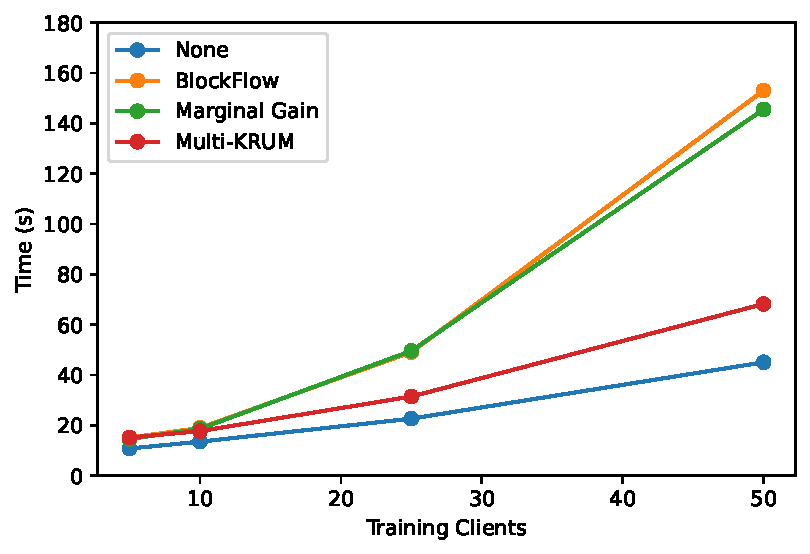
\includegraphics[width=\textwidth]{graphics/clients/round.pdf}
        \caption{Mean Round Time}
    \end{subfigure}
    \hfill
    \begin{subfigure}[b]{0.49\textwidth}
        \centering
        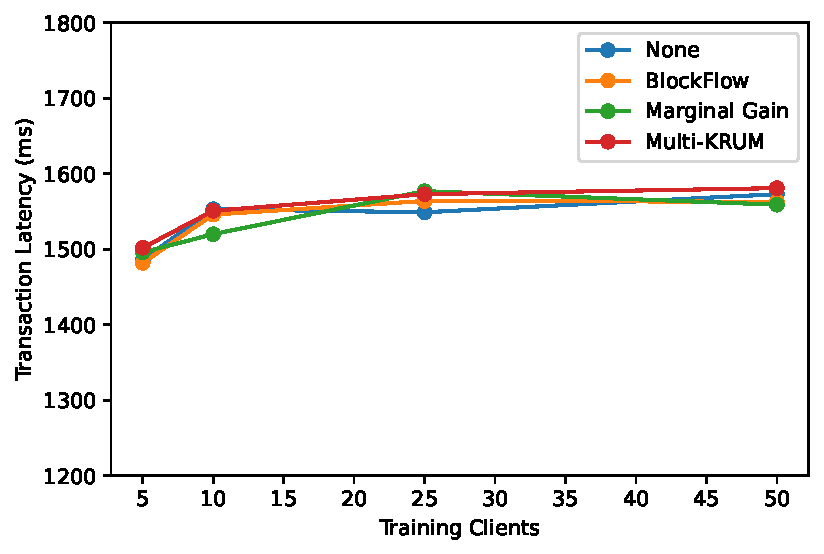
\includegraphics[width=\textwidth]{graphics/clients/tx_latency.pdf}
        \caption{Transaction Latency}
    \end{subfigure}
    \hfill
    \begin{subfigure}[b]{0.49\textwidth}
        \centering
        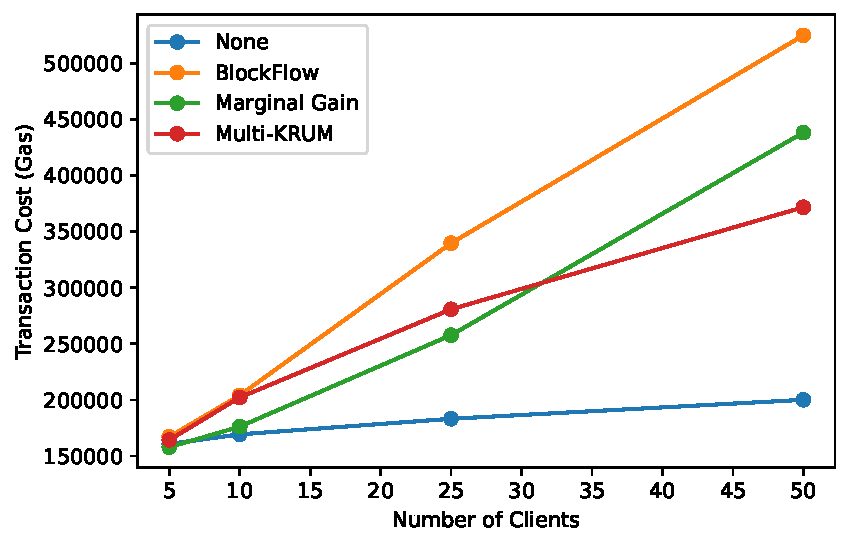
\includegraphics[width=\textwidth]{graphics/clients/tx_cost.pdf}
        \caption{Transaction Cost}
    \end{subfigure}
    \caption{Time and Transaction Metrics Per Training Clients}
    \label{fig:clients_metrics}
\end{figure}

\section{Accuracy and Convergence}

\begin{figure}[!ht]
    \centering
    \begin{subfigure}[b]{0.49\textwidth}
        \centering
        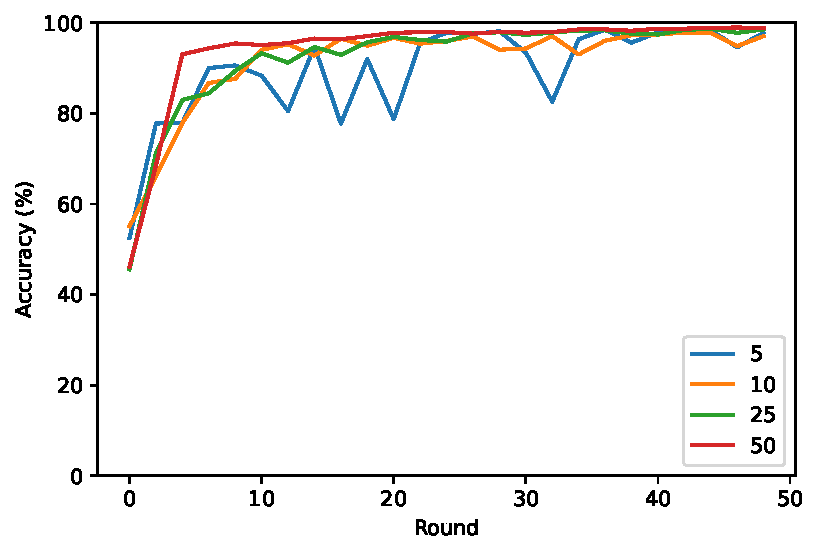
\includegraphics[width=\textwidth]{graphics/clients/accuracy_none.pdf}
        \caption{None}
    \end{subfigure}
    \hfill
    \begin{subfigure}[b]{0.49\textwidth}
        \centering
        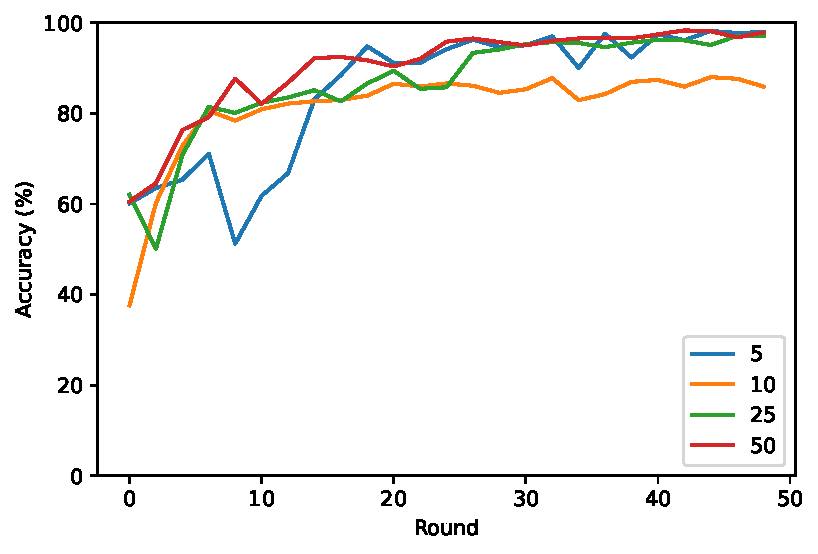
\includegraphics[width=\textwidth]{graphics/clients/accuracy_blockflow.pdf}
        \caption{BlockFlow}
    \end{subfigure}
    \hfill
    \begin{subfigure}[b]{0.49\textwidth}
        \centering
        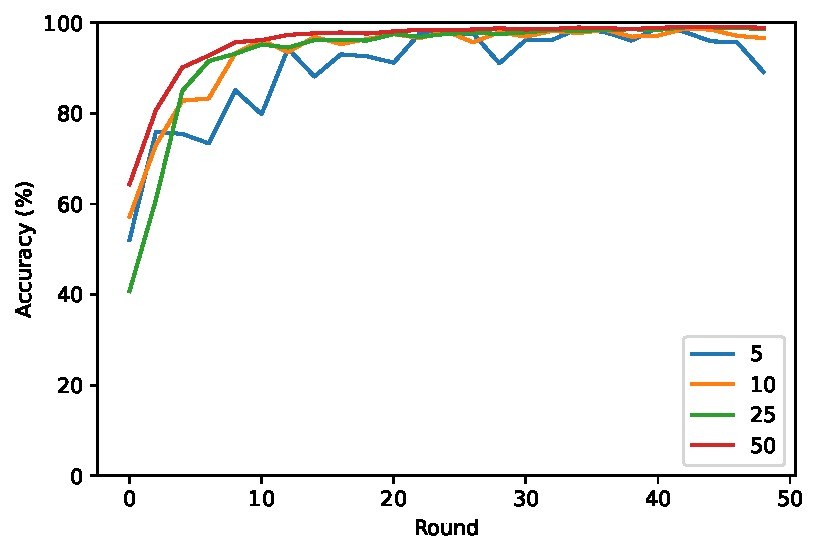
\includegraphics[width=\textwidth]{graphics/clients/accuracy_marginalgain.pdf}
        \caption{Marginal Gain}
    \end{subfigure}
    \hfill
    \begin{subfigure}[b]{0.49\textwidth}
        \centering
        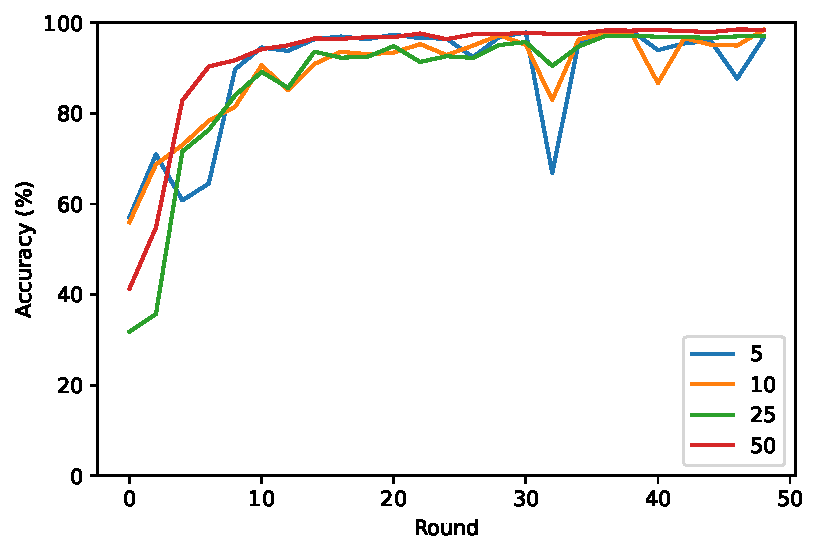
\includegraphics[width=\textwidth]{graphics/clients/accuracy_multikrum.pdf}
        \caption{Multi-KRUM}
    \end{subfigure}
    \caption{Accuracy Per Training Clients}
    \label{fig:clients_accuracy}
\end{figure}

\section{Communication Costs}

\begin{figure}[!ht]
    \centering
    \begin{subfigure}[b]{0.49\textwidth}
        \centering
        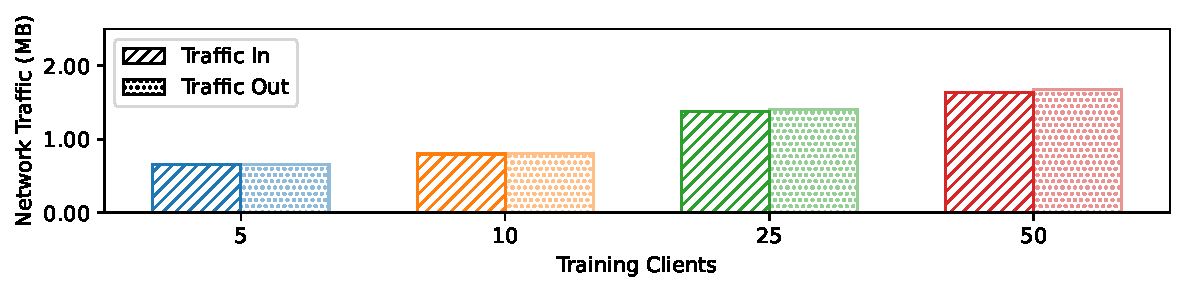
\includegraphics[width=\textwidth]{graphics/clients/net_none_client.pdf}
        \caption{None}
    \end{subfigure}
    \hfill
    \begin{subfigure}[b]{0.49\textwidth}
        \centering
        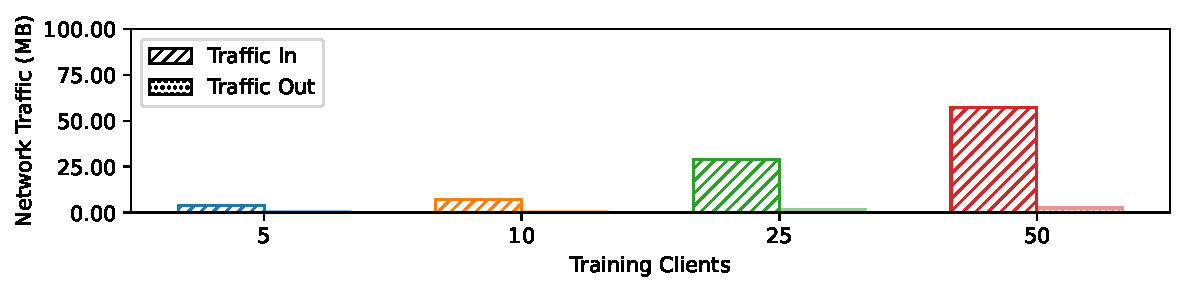
\includegraphics[width=\textwidth]{graphics/clients/net_blockflow_client.pdf}
        \caption{BlockFlow}
    \end{subfigure}
    \hfill
    \begin{subfigure}[b]{0.49\textwidth}
        \centering
        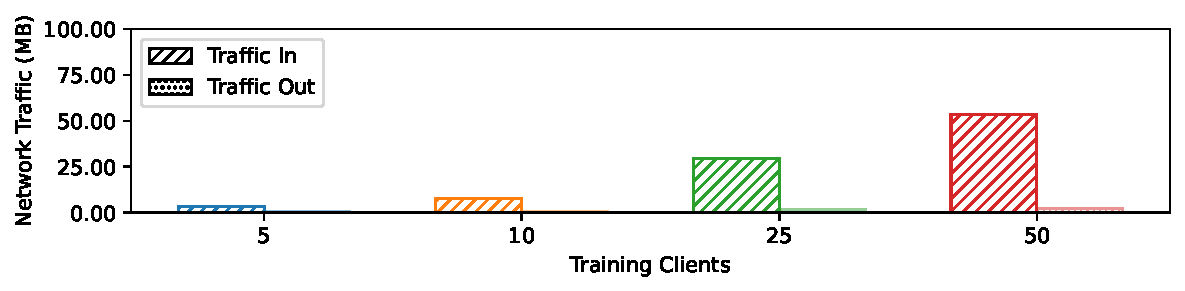
\includegraphics[width=\textwidth]{graphics/clients/net_marginalgain_client.pdf}
        \caption{Marginal Gain}
    \end{subfigure}
    \hfill
    \begin{subfigure}[b]{0.49\textwidth}
        \centering
        \includegraphics[width=\textwidth]{graphics/clients/net_multikrum_client.pdf}
        \caption{Multi-KRUM}
    \end{subfigure}
    \caption{Network Traffic on Training Clients Per Training Clients}
    \label{fig:net_clients_degree_clients}
\end{figure}

\begin{figure}[!ht]
    \centering
    \begin{subfigure}[b]{0.49\textwidth}
        \centering
        \includegraphics[width=\textwidth]{graphics/clients/net_none_server.pdf}
        \caption{None}
    \end{subfigure}
    \hfill
    \begin{subfigure}[b]{0.49\textwidth}
        \centering
        \includegraphics[width=\textwidth]{graphics/clients/net_blockflow_server.pdf}
        \caption{BlockFlow}
    \end{subfigure}
    \hfill
    \begin{subfigure}[b]{0.49\textwidth}
        \centering
        \includegraphics[width=\textwidth]{graphics/clients/net_marginalgain_server.pdf}
        \caption{Marginal Gain}
    \end{subfigure}
    \hfill
    \begin{subfigure}[b]{0.49\textwidth}
        \centering
        \includegraphics[width=\textwidth]{graphics/clients/net_multikrum_server.pdf}
        \caption{Multi-KRUM}
    \end{subfigure}
    \caption{Network Traffic on Computing Servers Per Training Clients}
    \label{fig:net_clients_degree_server}
\end{figure}

\begin{figure}[!ht]
    \centering
    \begin{subfigure}[b]{0.49\textwidth}
        \centering
        \includegraphics[width=\textwidth]{graphics/clients/net_none_miner.pdf}
        \caption{None}
    \end{subfigure}
    \hfill
    \begin{subfigure}[b]{0.49\textwidth}
        \centering
        \includegraphics[width=\textwidth]{graphics/clients/net_blockflow_miner.pdf}
        \caption{BlockFlow}
    \end{subfigure}
    \hfill
    \begin{subfigure}[b]{0.49\textwidth}
        \centering
        \includegraphics[width=\textwidth]{graphics/clients/net_marginalgain_miner.pdf}
        \caption{Marginal Gain}
    \end{subfigure}
    \hfill
    \begin{subfigure}[b]{0.49\textwidth}
        \centering
        \includegraphics[width=\textwidth]{graphics/clients/net_multikrum_miner.pdf}
        \caption{Multi-KRUM}
    \end{subfigure}
    \caption{Network Traffic on Blockchain Nodes Per Training Clients}
    \label{fig:net_clients_degree_miner}
\end{figure}

\section{Computation Costs}

\begin{figure}[!ht]
    \centering
    \begin{subfigure}[b]{0.49\textwidth}
        \centering
        \includegraphics[width=\textwidth]{graphics/clients/ram_none_client.pdf}
        \caption{None}
    \end{subfigure}
    \hfill
    \begin{subfigure}[b]{0.49\textwidth}
        \centering
        \includegraphics[width=\textwidth]{graphics/clients/ram_blockflow_client.pdf}
        \caption{BlockFlow}
    \end{subfigure}
    \hfill
    \begin{subfigure}[b]{0.49\textwidth}
        \centering
        \includegraphics[width=\textwidth]{graphics/clients/ram_marginalgain_client.pdf}
        \caption{Marginal Gain}
    \end{subfigure}
    \hfill
    \begin{subfigure}[b]{0.49\textwidth}
        \centering
        \includegraphics[width=\textwidth]{graphics/clients/ram_multikrum_client.pdf}
        \caption{Multi-KRUM}
    \end{subfigure}
    \caption{RAM Usage on Training Clients Per Training Clients}
    \label{fig:ram_clients_degree_clients}
\end{figure}

\begin{figure}[!ht]
    \centering
    \begin{subfigure}[b]{0.49\textwidth}
        \centering
        \includegraphics[width=\textwidth]{graphics/clients/ram_none_server.pdf}
        \caption{None}
    \end{subfigure}
    \hfill
    \begin{subfigure}[b]{0.49\textwidth}
        \centering
        \includegraphics[width=\textwidth]{graphics/clients/ram_blockflow_server.pdf}
        \caption{BlockFlow}
    \end{subfigure}
    \hfill
    \begin{subfigure}[b]{0.49\textwidth}
        \centering
        \includegraphics[width=\textwidth]{graphics/clients/ram_marginalgain_server.pdf}
        \caption{Marginal Gain}
    \end{subfigure}
    \hfill
    \begin{subfigure}[b]{0.49\textwidth}
        \centering
        \includegraphics[width=\textwidth]{graphics/clients/ram_multikrum_server.pdf}
        \caption{Multi-KRUM}
    \end{subfigure}
    \caption{RAM Usage on Computing Servers Per Training Clients}
    \label{fig:ram_clients_degree_server}
\end{figure}

\begin{figure}[!ht]
    \centering
    \begin{subfigure}[b]{0.49\textwidth}
        \centering
        \includegraphics[width=\textwidth]{graphics/clients/ram_none_miner.pdf}
        \caption{None}
    \end{subfigure}
    \hfill
    \begin{subfigure}[b]{0.49\textwidth}
        \centering
        \includegraphics[width=\textwidth]{graphics/clients/ram_blockflow_miner.pdf}
        \caption{BlockFlow}
    \end{subfigure}
    \hfill
    \begin{subfigure}[b]{0.49\textwidth}
        \centering
        \includegraphics[width=\textwidth]{graphics/clients/ram_marginalgain_miner.pdf}
        \caption{Marginal Gain}
    \end{subfigure}
    \hfill
    \begin{subfigure}[b]{0.49\textwidth}
        \centering
        \includegraphics[width=\textwidth]{graphics/clients/ram_multikrum_miner.pdf}
        \caption{Multi-KRUM}
    \end{subfigure}
    \caption{RAM Usage on Blockchain Nodes Per Training Clients}
    \label{fig:ram_clients_degree_miner}
\end{figure}






\begin{figure}[!ht]
    \centering
    \begin{subfigure}[b]{0.49\textwidth}
        \centering
        \includegraphics[width=\textwidth]{graphics/clients/cpu_none_client.pdf}
        \caption{None}
    \end{subfigure}
    \hfill
    \begin{subfigure}[b]{0.49\textwidth}
        \centering
        \includegraphics[width=\textwidth]{graphics/clients/cpu_blockflow_client.pdf}
        \caption{BlockFlow}
    \end{subfigure}
    \hfill
    \begin{subfigure}[b]{0.49\textwidth}
        \centering
        \includegraphics[width=\textwidth]{graphics/clients/cpu_marginalgain_client.pdf}
        \caption{Marginal Gain}
    \end{subfigure}
    \hfill
    \begin{subfigure}[b]{0.49\textwidth}
        \centering
        \includegraphics[width=\textwidth]{graphics/clients/cpu_multikrum_client.pdf}
        \caption{Multi-KRUM}
    \end{subfigure}
    \caption{CPU Usage on Training Clients Per Training Clients}
    \label{fig:cpu_clients_degree_clients}
\end{figure}

\begin{figure}[!ht]
    \centering
    \begin{subfigure}[b]{0.49\textwidth}
        \centering
        \includegraphics[width=\textwidth]{graphics/clients/cpu_none_server.pdf}
        \caption{None}
    \end{subfigure}
    \hfill
    \begin{subfigure}[b]{0.49\textwidth}
        \centering
        \includegraphics[width=\textwidth]{graphics/clients/cpu_blockflow_server.pdf}
        \caption{BlockFlow}
    \end{subfigure}
    \hfill
    \begin{subfigure}[b]{0.49\textwidth}
        \centering
        \includegraphics[width=\textwidth]{graphics/clients/cpu_marginalgain_server.pdf}
        \caption{Marginal Gain}
    \end{subfigure}
    \hfill
    \begin{subfigure}[b]{0.49\textwidth}
        \centering
        \includegraphics[width=\textwidth]{graphics/clients/cpu_multikrum_server.pdf}
        \caption{Multi-KRUM}
    \end{subfigure}
    \caption{CPU Usage on Computing Servers Per Training Clients}
    \label{fig:cpu_clients_degree_server}
\end{figure}

\begin{figure}[!ht]
    \centering
    \begin{subfigure}[b]{0.49\textwidth}
        \centering
        \includegraphics[width=\textwidth]{graphics/clients/cpu_none_miner.pdf}
        \caption{None}
    \end{subfigure}
    \hfill
    \begin{subfigure}[b]{0.49\textwidth}
        \centering
        \includegraphics[width=\textwidth]{graphics/clients/cpu_blockflow_miner.pdf}
        \caption{BlockFlow}
    \end{subfigure}
    \hfill
    \begin{subfigure}[b]{0.49\textwidth}
        \centering
        \includegraphics[width=\textwidth]{graphics/clients/cpu_marginalgain_miner.pdf}
        \caption{Marginal Gain}
    \end{subfigure}
    \hfill
    \begin{subfigure}[b]{0.49\textwidth}
        \centering
        \includegraphics[width=\textwidth]{graphics/clients/cpu_multikrum_miner.pdf}
        \caption{Multi-KRUM}
    \end{subfigure}
    \caption{CPU Usage on Blockchain Nodes Per Training Clients}
    \label{fig:cpu_clients_degree_miner}
\end{figure}

\section{Conclusions} % and improvements? and limitations?


% \chapter{Impact Analysis of Privacy Degrees}\label{chapter:analysis:privacy}
% In this chapter, we analyze the fifth experiment group, that is, the impact of having different degrees of privacy, per scoring technique, in a Blockchain-based Federated Learning system. In this set of experiments, all properties of the system are static, except for the degree of privacy, which varies between 0, 1 and 5, per each scoring mechanism.

\todo{}

\section{Execution Time, Transaction Cost and Latency}

\begin{figure}[!ht]
    \centering
    \begin{subfigure}[b]{0.49\textwidth}
        \centering
        \includegraphics[width=\textwidth]{graphics/privacy/e2e.pdf}
        \caption{E2E Time}
    \end{subfigure}
    \hfill
    \begin{subfigure}[b]{0.49\textwidth}
        \centering
        \includegraphics[width=\textwidth]{graphics/privacy/round.pdf}
        \caption{Mean Round Time}
    \end{subfigure}
    \hfill
    \begin{subfigure}[b]{0.49\textwidth}
        \centering
        \includegraphics[width=\textwidth]{graphics/privacy/tx_latency.pdf}
        \caption{Transaction Latency}
    \end{subfigure}
    \hfill
    \begin{subfigure}[b]{0.49\textwidth}
        \centering
        \includegraphics[width=\textwidth]{graphics/privacy/tx_cost.pdf}
        \caption{Transaction Cost}
    \end{subfigure}
    \caption{Time and Transaction Metrics Per Privacy Degree}
    \label{fig:priv_metrics}
\end{figure}

\section{Accuracy and Convergence}

\begin{figure}[!ht]
    \centering
    \begin{subfigure}[b]{0.49\textwidth}
        \centering
        \includegraphics[width=\textwidth]{graphics/privacy/accuracy_none.pdf}
        \caption{None}
    \end{subfigure}
    \hfill
    \begin{subfigure}[b]{0.49\textwidth}
        \centering
        \includegraphics[width=\textwidth]{graphics/privacy/accuracy_blockflow.pdf}
        \caption{BlockFlow}
    \end{subfigure}
    \hfill
    \begin{subfigure}[b]{0.49\textwidth}
        \centering
        \includegraphics[width=\textwidth]{graphics/privacy/accuracy_marginalgain.pdf}
        \caption{Marginal Gain}
    \end{subfigure}
    \hfill
    \begin{subfigure}[b]{0.49\textwidth}
        \centering
        \includegraphics[width=\textwidth]{graphics/privacy/accuracy_multikrum.pdf}
        \caption{Multi-KRUM}
    \end{subfigure}
    \caption{Accuracy Per Privacy Degree}
    \label{fig:accuracy_priv}
\end{figure}

\section{Communication Costs}


\begin{figure}[!ht]
    \centering
    \begin{subfigure}[b]{0.49\textwidth}
        \centering
        \includegraphics[width=\textwidth]{graphics/privacy/net_none_client.pdf}
        \caption{None}
    \end{subfigure}
    \hfill
    \begin{subfigure}[b]{0.49\textwidth}
        \centering
        \includegraphics[width=\textwidth]{graphics/privacy/net_blockflow_client.pdf}
        \caption{BlockFlow}
    \end{subfigure}
    \hfill
    \begin{subfigure}[b]{0.49\textwidth}
        \centering
        \includegraphics[width=\textwidth]{graphics/privacy/net_marginalgain_client.pdf}
        \caption{Marginal Gain}
    \end{subfigure}
    \hfill
    \begin{subfigure}[b]{0.49\textwidth}
        \centering
        \includegraphics[width=\textwidth]{graphics/privacy/net_multikrum_client.pdf}
        \caption{Multi-KRUM}
    \end{subfigure}
    \caption{Network Traffic on Training Clients Per Privacy Degree}
    \label{fig:net_priv_degree_clients}
\end{figure}

\begin{figure}[!ht]
    \centering
    \begin{subfigure}[b]{0.49\textwidth}
        \centering
        \includegraphics[width=\textwidth]{graphics/privacy/net_none_server.pdf}
        \caption{None}
    \end{subfigure}
    \hfill
    \begin{subfigure}[b]{0.49\textwidth}
        \centering
        \includegraphics[width=\textwidth]{graphics/privacy/net_blockflow_server.pdf}
        \caption{BlockFlow}
    \end{subfigure}
    \hfill
    \begin{subfigure}[b]{0.49\textwidth}
        \centering
        \includegraphics[width=\textwidth]{graphics/privacy/net_marginalgain_server.pdf}
        \caption{Marginal Gain}
    \end{subfigure}
    \hfill
    \begin{subfigure}[b]{0.49\textwidth}
        \centering
        \includegraphics[width=\textwidth]{graphics/privacy/net_multikrum_server.pdf}
        \caption{Multi-KRUM}
    \end{subfigure}
    \caption{Network Traffic on Computing Servers Per Privacy Degree}
    \label{fig:net_priv_degree_server}
\end{figure}

\begin{figure}[!ht]
    \centering
    \begin{subfigure}[b]{0.49\textwidth}
        \centering
        \includegraphics[width=\textwidth]{graphics/privacy/net_none_miner.pdf}
        \caption{None}
    \end{subfigure}
    \hfill
    \begin{subfigure}[b]{0.49\textwidth}
        \centering
        \includegraphics[width=\textwidth]{graphics/privacy/net_blockflow_miner.pdf}
        \caption{BlockFlow}
    \end{subfigure}
    \hfill
    \begin{subfigure}[b]{0.49\textwidth}
        \centering
        \includegraphics[width=\textwidth]{graphics/privacy/net_marginalgain_miner.pdf}
        \caption{Marginal Gain}
    \end{subfigure}
    \hfill
    \begin{subfigure}[b]{0.49\textwidth}
        \centering
        \includegraphics[width=\textwidth]{graphics/privacy/net_multikrum_miner.pdf}
        \caption{Multi-KRUM}
    \end{subfigure}
    \caption{Network Traffic on Blockchain Nodes Per Privacy Degree}
    \label{fig:net_priv_degree_miner}
\end{figure}

\section{Computation Costs}

\begin{figure}[!ht]
    \centering
    \begin{subfigure}[b]{0.49\textwidth}
        \centering
        \includegraphics[width=\textwidth]{graphics/privacy/ram_none_client.pdf}
        \caption{None}
    \end{subfigure}
    \hfill
    \begin{subfigure}[b]{0.49\textwidth}
        \centering
        \includegraphics[width=\textwidth]{graphics/privacy/ram_blockflow_client.pdf}
        \caption{BlockFlow}
    \end{subfigure}
    \hfill
    \begin{subfigure}[b]{0.49\textwidth}
        \centering
        \includegraphics[width=\textwidth]{graphics/privacy/ram_marginalgain_client.pdf}
        \caption{Marginal Gain}
    \end{subfigure}
    \hfill
    \begin{subfigure}[b]{0.49\textwidth}
        \centering
        \includegraphics[width=\textwidth]{graphics/privacy/ram_multikrum_client.pdf}
        \caption{Multi-KRUM}
    \end{subfigure}
    \caption{RAM Usage on Training Clients Per Privacy Degree}
    \label{fig:ram_priv_degree_clients}
\end{figure}

\begin{figure}[!ht]
    \centering
    \begin{subfigure}[b]{0.49\textwidth}
        \centering
        \includegraphics[width=\textwidth]{graphics/privacy/ram_none_server.pdf}
        \caption{None}
    \end{subfigure}
    \hfill
    \begin{subfigure}[b]{0.49\textwidth}
        \centering
        \includegraphics[width=\textwidth]{graphics/privacy/ram_blockflow_server.pdf}
        \caption{BlockFlow}
    \end{subfigure}
    \hfill
    \begin{subfigure}[b]{0.49\textwidth}
        \centering
        \includegraphics[width=\textwidth]{graphics/privacy/ram_marginalgain_server.pdf}
        \caption{Marginal Gain}
    \end{subfigure}
    \hfill
    \begin{subfigure}[b]{0.49\textwidth}
        \centering
        \includegraphics[width=\textwidth]{graphics/privacy/ram_multikrum_server.pdf}
        \caption{Multi-KRUM}
    \end{subfigure}
    \caption{RAM Usage on Computing Servers Per Privacy Degree}
    \label{fig:ram_priv_degree_server}
\end{figure}

\begin{figure}[!ht]
    \centering
    \begin{subfigure}[b]{0.49\textwidth}
        \centering
        \includegraphics[width=\textwidth]{graphics/privacy/ram_none_miner.pdf}
        \caption{None}
    \end{subfigure}
    \hfill
    \begin{subfigure}[b]{0.49\textwidth}
        \centering
        \includegraphics[width=\textwidth]{graphics/privacy/ram_blockflow_miner.pdf}
        \caption{BlockFlow}
    \end{subfigure}
    \hfill
    \begin{subfigure}[b]{0.49\textwidth}
        \centering
        \includegraphics[width=\textwidth]{graphics/privacy/ram_marginalgain_miner.pdf}
        \caption{Marginal Gain}
    \end{subfigure}
    \hfill
    \begin{subfigure}[b]{0.49\textwidth}
        \centering
        \includegraphics[width=\textwidth]{graphics/privacy/ram_multikrum_miner.pdf}
        \caption{Multi-KRUM}
    \end{subfigure}
    \caption{RAM Usage on Blockchain Nodes Per Privacy Degree}
    \label{fig:ram_priv_degree_miner}
\end{figure}






\begin{figure}[!ht]
    \centering
    \begin{subfigure}[b]{0.49\textwidth}
        \centering
        \includegraphics[width=\textwidth]{graphics/privacy/cpu_none_client.pdf}
        \caption{None}
    \end{subfigure}
    \hfill
    \begin{subfigure}[b]{0.49\textwidth}
        \centering
        \includegraphics[width=\textwidth]{graphics/privacy/cpu_blockflow_client.pdf}
        \caption{BlockFlow}
    \end{subfigure}
    \hfill
    \begin{subfigure}[b]{0.49\textwidth}
        \centering
        \includegraphics[width=\textwidth]{graphics/privacy/cpu_marginalgain_client.pdf}
        \caption{Marginal Gain}
    \end{subfigure}
    \hfill
    \begin{subfigure}[b]{0.49\textwidth}
        \centering
        \includegraphics[width=\textwidth]{graphics/privacy/cpu_multikrum_client.pdf}
        \caption{Multi-KRUM}
    \end{subfigure}
    \caption{CPU Usage on Training Clients Per Privacy Degree}
    \label{fig:cpu_priv_degree_clients}
\end{figure}

\begin{figure}[!ht]
    \centering
    \begin{subfigure}[b]{0.49\textwidth}
        \centering
        \includegraphics[width=\textwidth]{graphics/privacy/cpu_none_server.pdf}
        \caption{None}
    \end{subfigure}
    \hfill
    \begin{subfigure}[b]{0.49\textwidth}
        \centering
        \includegraphics[width=\textwidth]{graphics/privacy/cpu_blockflow_server.pdf}
        \caption{BlockFlow}
    \end{subfigure}
    \hfill
    \begin{subfigure}[b]{0.49\textwidth}
        \centering
        \includegraphics[width=\textwidth]{graphics/privacy/cpu_marginalgain_server.pdf}
        \caption{Marginal Gain}
    \end{subfigure}
    \hfill
    \begin{subfigure}[b]{0.49\textwidth}
        \centering
        \includegraphics[width=\textwidth]{graphics/privacy/cpu_multikrum_server.pdf}
        \caption{Multi-KRUM}
    \end{subfigure}
    \caption{CPU Usage on Computing Servers Per Privacy Degree}
    \label{fig:cpu_priv_degree_server}
\end{figure}

\begin{figure}[!ht]
    \centering
    \begin{subfigure}[b]{0.49\textwidth}
        \centering
        \includegraphics[width=\textwidth]{graphics/privacy/cpu_none_miner.pdf}
        \caption{None}
    \end{subfigure}
    \hfill
    \begin{subfigure}[b]{0.49\textwidth}
        \centering
        \includegraphics[width=\textwidth]{graphics/privacy/cpu_blockflow_miner.pdf}
        \caption{BlockFlow}
    \end{subfigure}
    \hfill
    \begin{subfigure}[b]{0.49\textwidth}
        \centering
        \includegraphics[width=\textwidth]{graphics/privacy/cpu_marginalgain_miner.pdf}
        \caption{Marginal Gain}
    \end{subfigure}
    \hfill
    \begin{subfigure}[b]{0.49\textwidth}
        \centering
        \includegraphics[width=\textwidth]{graphics/privacy/cpu_multikrum_miner.pdf}
        \caption{Multi-KRUM}
    \end{subfigure}
    \caption{CPU Usage on Blockchain Nodes Per Privacy Degree}
    \label{fig:cpu_priv_degree_miner}
\end{figure}

\section{Conclusions} % and improvements? and limitations?


\chapter{Proof of Concept of Vertical Blockchain-based Federated Learning}\label{chapter:vertical}
In this chapter, we analyze the sixth and last experiment group, that is, the proof of concept of Vertical Blockchain-based Federated Learning. The goal of this experiment is to prove that, even though there is a lack of Blockchain-based Federated Learning systems applied to vertically partitioned data, it is possible.

This experiment was run with two different amounts of clients: 2 and 4, with a dual-headed, and four-headed, Split-CNN model, respectively. By having two experiments in this group, we can still draw some comparisons. In addition, most Vertical Federated Learning models from the literature were applied to 2 clients. Therefore, it is interesting to see that it is possible to easily apply the model to more clients.

\section{Execution Time, Transaction Cost and Latency}

The execution time and transaction metrics can be seen in \autoref{tab:metrics_vertical}. It is observable that the more clients we have, the longest it takes for a round to be completed and, therefore, the entire learning process. This is a conclusion that was taken in a previous chapter too.

Regarding the transaction latency and cost, we can see that both are similar to what has been seen in previous chapters. Since the number of clients is low, we did not expect to have significant differences in either of them.

\begin{table}[!ht]
\begin{tabular}{c|c|c} \hline \hline
                                & 2             & 4             \\ \hline \hline
E2E Time (m)                    & 10.97	        & 12.57         \\ \hline
Mean Round Time (s)             & 13.16	        & 15.08         \\ \hline
Mean Transaction Latency (s)    & 1.642	        & 1.546         \\ \hline
Mean Transaction Cost (Gas)     & 141335        & 142638        \\ \hline
\end{tabular}
\caption{Time and Transaction Metrics Per Number of Clients}
\label{tab:metrics_vertical}
\end{table}

\section{Accuracy and Convergence}

Regarding accuracy, we can observe smooth convergences, as well as similar high accuracy. Both clients reached an accuracy above $85\%$, only differing in $3\%$. In addition, it is interesting to see that the convergence of the Vertical Federated Learning is much smoother than what we have observed with Horizontal Federated Learning. This is likely explained by the fact that in this setting, all clients participate in each round due to the way the data is structured. In addition, the model is different from a regular CNN, which may lead to different results. However, since both types of data partition solve different types of problems, it is not a fair comparison.

\begin{figure}[!ht]
    \centering
    \centering
    \includegraphics[width=0.7\textwidth]{graphics/vertical/accuracy.pdf}
    \caption{Accuracy Per Number of Clients}
    \label{fig:accuracy_vertical}
\end{figure}

\section{Communication Costs}

The communication costs represented in \autoref{fig:net_vertical} are also within the expected values.

On the clients, we can observe that there is no major difference of traffic when the number of clients increases. This can be explained by the fact that, by using a Split-CNN, each client is only required to upload their own intermediate results and download the gradient updates, which have fixed sizes.

On the servers, the costs are higher with more clients. Since the Split-CNN model has more heads with more clients, the servers are required to download more intermediate results, as well as upload more gradient updates. Therefore, it would be expected that the traffic would double with the double of clients.

On the blockchain, the difference of amount of clients is not significant to make a significant difference on traffic.

\begin{figure}[!ht]
    \centering
    \centering
    \includegraphics[width=0.8\textwidth]{graphics/vertical/net.pdf}
    \caption{Network Traffic Per Round Per Number of Clients}
    \label{fig:net_vertical}
\end{figure}

\section{Computation Costs}

Computation costs, namely RAM usage and CPU usage, are depicted in \autoref{fig:ram_vertical} and \autoref{fig:cpu_vertical}, respectively. As expected, with higher amounts of clients there is a slightly higher RAM consumption on both the server and blockchain processes, caused by more data being stored in-memory, as well as more messages being carried over the blockchain. However, we see the opposite happening with the clients. This is explained by the fact that the dual-headed CNN contains an additional convolutional layer compared to the four-headed CNN, which leads to more RAM usage during training. Regarding CPU usage, we see similar results as to the RAM usage, which are explained by the same reasons.

\begin{figure}[!ht]
    \centering
    \centering
    \includegraphics[width=0.8\textwidth]{graphics/vertical/ram.pdf}
    \caption{RAM Usage Per Number of Clients}
    \label{fig:ram_vertical}
\end{figure}

\begin{figure}[!ht]
    \centering
    \centering
    \includegraphics[width=0.8\textwidth]{graphics/vertical/cpu.pdf}
    \caption{CPU Usage Per Number of Clients}
    \label{fig:cpu_vertical}
\end{figure}

\section{Conclusions and Improvements}

From this experiment, we can conclude that it is possible to apply a Blockchain-based Federated Learning system to vertically partitioned data. In future work, it would be interesting to investigate how to apply other models. In addition, it would be interesting to see how other, larger data sets, could be applied with larger amounts of clients. Using MNIST, this experiment is limited because of the extremely small resolution of the images. Therefore, it is not feasible to separate many features. Finally, it would also be worth investigating how privacy mechanisms could be applied to the intermediate model outputs in order to prevent inference attacks.


\chapter{Conclusion}\label{chapter:conclusion}
BFL was initially introduced in order to facilitate desirable properties such as traceability, auditability, immutability, persistency, authentication and decentralization. Even though applying blockchain to a Federated Learning system brings these advantages, it also brings some trade-offs. Therefore, in this thesis, we explored how different algorithms used in Blockchain-based Federated Learning (BFL) systems impact the system 's performance in terms of execution time, accuracy and resource consumption. 

Our analysis of related work revealed that even though there are many works on designing BFL frameworks, a very few of them are
released to the public, or are modular. We, therefore, designed and implemented the very first open-source modular BFL framework that allows many aspects of the system to be easily customized and supports multiple architectures. By making it available to the public, it has the potential to empower future research.

\section{Observations From our Impact Analysis}\label{conclusions:evaluation}



Firstly, we analyzed the impact of different consensus algorithms, i.e., POW, POA, and QBFT. We concluded that different consensus algorithms play a large role in the energy consumption. In terms of computation costs, the PoW algorithm presented the highest consumption, while QBFT and PoA presented lower consumption. Regarding communication costs, QBFT had up to three times more network traffic compared to its counterparts. Consequently, we concluded that the PoA algorithm is the most cost-efficient algorithm. However, it is criticized for the degree of decentralization it provides due to the way the validator nodes are chosen. Therefore, we concluded that there is a \textit{trade-off between the degree of decentralization and the energy costs of the consensus algorithm}.

In third place, we analyzed the impact of different participant selection algorithms, which revealed to be similar in terms of energy consumption. However, randomly selecting participants revealed to be fairer and provide more stable accuracy convergence, as it gives every client an equal chance of participating in a round as long as the randomness is provided by a uniform distribution.

In fourth place, the scoring algorithms were analyzed. The scoring algorithms are required in order to filter worse contributions and prevent attacks, such as poisoning and plagiarism attacks. In addition, the scores are often used in order to give each client a reward for their contribution in order to incentive the client to participate. By adding a scoring algorithm, the execution time will increase up to twice as much, depending on whether the scoring algorithm is executed at the clients or the servers. There is a clear \textit{trade-off between the different kinds of scoring algorithms and the execution time and energy consumption, at both the clients and servers}.

In fifth place, we analyzed the impact of the number of clients and the privacy degrees on each scoring algorithm. We concluded that Marginal Gain is the most resilient to both, but also the one that consumes the most energy at the clients. Multi-KRUM revealed to be a good alternative in case the clients are low-powered devices and their communication and computations should be minimized. Finally, BlockFlow revealed to perform the worst in all aspects. We can conclude that there is a \textit{trade-off between accuracy and resiliency, and the resource consumption at the clients}.

In sixth, we provided a proof of concept of how Vertical Federated Learning can be applied to a BFL system.

\section{Looking Back to the Main Research Question}\label{conclusions:general}

The main research question of this thesis was \textit{"What is the impact of different consensus, participant selection and scoring algorithms in a Blockchain-based Federated Learning system on execution time, convergence and accuracy, as well as communication and computation costs?"}. 

Overall, our extensive experiments answered this by revealing that the addition of the blockchain, namely Ethereum, has impacts both in terms of execution time and resource usage. The average transaction latency we observed was around $1.5$ seconds. In each round, there are at least $C+S+2$ transactions, where $C$ and $S$ are the number of clients, and servers, respectively. Even though the clients and the servers execute their process in parallel, the transactions latency add up, increasing the execution time. Therefore, we conclude there is a general \textit{trade-off between the benefits of the blockchain and the execution time}.

After all, when adding the blockchain, we are adding a new layer to a system that would otherwise have a single centralized server. In order to achieve decentralization, we require more than one machine to replace the central server. Moreover, this machines must reach a consensus in terms of storage and execution. The costs of getting a system that provides traceability, auditability, immutability, persistency, authentication and decentralization are translated in higher energy costs and execution times.

% It is important (maybe not as we mentioned this before) to refer that, as mentioned previously in this work, there are other architectures. For example, in some architectures the clients are also the servers and the blockchain nodes. That is, the same machines execute all of the processing. However, this would not be feasible in an IoT system, or any other system where low-powered devices are the norm.


\section{Future Work}\label{conclusions:future_work}

Firstly, it would be interesting to build a GUI for BlockLearning that, not only allows to submit new training requests, but also provides an interactive way of visualizing the steps of the process, as well as transactions and communications.

Secondly, it would be worth investigating more methods of scoring algorithms that do not require evaluating the model with them. Both Marginal Gain and BlockFlow require that the model is evaluated by the clients, which consumes more resources and takes some time. On the other hand, Multi-KRUM scores updates by comparing the weight values directly. It would be interesting to see if such a method could be applied on the clients and if would bring the resource consumption down at the clients.

Finally, research in Blockchain-based Vertical Federated Learning should continue. Vertical Federated Learning solves a unique problem where multiple parties have different features on the same samples. The proof of concept provided in this work uses a very specific model that would not be applicable to many use cases. Therefore, more work into different types of model and architectures is required in order to understand the full potential.


\bibliographystyle{acm}
\bibliography{literature}

\appendix 
\addcontentsline{toc}{chapter}{Appendix}

\chapter{Horizontal Experiments}\label{chapter:horizontal_appendix}
\section{Participant Selection Algorithms}

\subsection{Communication Costs}

\vfill

\begin{figure}[!h]
    \centering
    \centering
    \includegraphics[width=0.8\textwidth]{graphics/selection/net.pdf}
    \caption{Network Traffic Per Round Per Participant Selection Algorithm}
    \label{fig:net_selection}
\end{figure}

\vfill

\clearpage

\subsection{Computation Costs}

\begin{figure}[!h]
    \centering
    \centering
    \includegraphics[width=0.8\textwidth]{graphics/selection/ram.pdf}
    \caption{RAM Usage Per Participant Selection Algorithm}
    \label{fig:ram_selection}
\end{figure}

\begin{figure}[!h]
    \centering
    \centering
    \includegraphics[width=0.8\textwidth]{graphics/selection/cpu.pdf}
    \caption{CPU Usage Per Participant Selection Algorithm}
    \label{fig:cpu_selection}
\end{figure}

\clearpage

\section{Scoring Algorithms}

\subsection{Communication Costs}

\vfill

\begin{figure}[!ht]
    \centering
    \centering
    \includegraphics[width=0.8\textwidth]{graphics/scoring/net.pdf}
    \caption{Network Traffic Per Round Per Scoring Algorithm}
    \label{fig:net_scoring}
\end{figure}

\vfill

\clearpage

\subsection{Computation Costs}

\begin{figure}[!hpt]
    \centering
    \centering
    \includegraphics[width=0.8\textwidth]{graphics/scoring/ram.pdf}
    \caption{RAM Usage Per Scoring Algorithm}
    \label{fig:ram_scoring}
\end{figure}

\begin{figure}[!hpb]
    \centering
    \centering
    \includegraphics[width=0.8\textwidth]{graphics/scoring/cpu.pdf}
    \caption{CPU Usage Per Scoring Algorithm}
    \label{fig:cpu_scoring}
\end{figure}

\clearpage

\subsection{Number of Clients}

\subsubsection{Computation Costs}

\begin{figure}[!h]
    \centering
    \includegraphics[width=\textwidth]{graphics/clients/ram_client.pdf}
    \caption{Client Process RAM Usage Per Number of Clients}
    \label{fig:ram_clients_clients}
\end{figure}

\begin{figure}[!h]
    \centering
    \includegraphics[width=\textwidth]{graphics/clients/ram_server.pdf}
    \caption{Server Process RAM Usage Per Number of Clients}
    \label{fig:ram_clients_servers}
\end{figure}

\begin{figure}[!h]
    \centering
    \includegraphics[width=\textwidth]{graphics/clients/ram_miner.pdf}
    \caption{Blockchain Process RAM Usage Per Number of Clients}
    \label{fig:ram_clients_miners}
\end{figure}

\clearpage

\begin{figure}[!h]
    \centering
    \includegraphics[width=\textwidth]{graphics/clients/cpu_client.pdf}
    \caption{Client Process CPU Usage Per Number of Clients}
    \label{fig:cpu_clients_clients}
\end{figure}

\begin{figure}[!h]
    \centering
    \includegraphics[width=\textwidth]{graphics/clients/cpu_server.pdf}
    \caption{Server Process CPU Usage Per Number of Clients}
    \label{fig:cpu_clients_servers}
\end{figure}

\begin{figure}[!h]
    \centering
    \includegraphics[width=\textwidth]{graphics/clients/cpu_miner.pdf}
    \caption{Blockchain Process CPU Usage Per Number of Clients}
    \label{fig:cpu_clients_miners}
\end{figure}

\clearpage

\subsection{Privacy Degrees}

\subsubsection{Communication Costs}

\vfill

\begin{figure}[!h]
    \centering
    \includegraphics[width=\textwidth]{graphics/privacy/traffic.pdf}
    \caption{Network Traffic Per Privacy Degree}
    \label{fig:net_privacy}
\end{figure}

\vfill

\clearpage

\subsubsection{Computation Costs}

\begin{figure}[!h]
    \centering
    \includegraphics[width=\textwidth]{graphics/privacy/ram_client.pdf}
    \caption{Client Process RAM Usage Per Privacy Degree}
    \label{fig:ram_privacy_clients}
\end{figure}

\begin{figure}[!h]
    \centering
    \includegraphics[width=\textwidth]{graphics/privacy/ram_server.pdf}
    \caption{Server Process RAM Usage Per Privacy Degree}
    \label{fig:ram_privacy_servers}
\end{figure}

\begin{figure}[!h]
    \centering
    \includegraphics[width=\textwidth]{graphics/privacy/ram_miner.pdf}
    \caption{Blockchain Process RAM Usage Per Privacy Degree}
    \label{fig:ram_privacy_miners}
\end{figure}

\clearpage

\begin{figure}[!h]
    \centering
    \includegraphics[width=\textwidth]{graphics/privacy/cpu_client.pdf}
    \caption{Client Process CPU Usage Per Privacy Degree}
    \label{fig:cpu_privacy_clients}
\end{figure}

\begin{figure}[!h]
    \centering
    \includegraphics[width=\textwidth]{graphics/privacy/cpu_server.pdf}
    \caption{Server Process CPU Usage Per Privacy Degree}
    \label{fig:cpu_privacy_servers}
\end{figure}

\begin{figure}[!h]
    \centering
    \includegraphics[width=\textwidth]{graphics/privacy/cpu_miner.pdf}
    \caption{Blockchain Process CPU Usage Per Privacy Degree}
    \label{fig:cpu_privacy_miners}
\end{figure}



\end{document}